% --------------------------
% CREDITS:
% I used the "UPM_thesis_template_en" template from Overaleaf and modified it to fit my needs for my final degree project.
% https://www.overleaf.com/latex/templates/upm-thesis-template-en/nzjnspqsxfmm
% --------------------------

% --------------------------
% Document class
% --------------------------
\documentclass[
twoside,                % onesite or twoside printing
openright,              % doublepage cleaning ends up right side
12pt,                   % font size
]{book}

% **************************************************
% THESIS details
% **************************************************

\newcommand{\University}{\protect{Universidad Polit\'ecnica de Madrid}}
\newcommand{\UNIVERSITY}{\protect{UNIVERSIDAD POLIT\'ECNICA DE MADRID}}

% **************************************************
% THESIS COVER DATA
% **************************************************
% Fill in the details of your thesis: author, title, etc. 

\newcommand{\thesisTitle}{\protect {Comparative analysis of computational performance in simulation with parallel processing techniques}}
\newcommand{\thesisAuthor}{\protect{Pedro Rodríguez Jiménez}}
% \newcommand{\priorstudies}{\protect{<Previous academic degree>}}
\newcommand{\thesisDate}{septiembre de 2025}

\newcommand{\UPMCentre}{\protect {Escuela Técnica Superior de\\Ingeniería Aeroespacial y del Espacio}}


\newcommand{\DoctoralProgramme}{Aerospace Engineering}

\newcommand{\supervisor}{Juan Antonio Hernández Ramos}
\newcommand{\cosupervisor}{Javier Luis González Monge}

\newcommand{\supervisorDetails}{<Supervisor Name and Surnames, position, institution> }
\newcommand{\cosupervisorDetails}{<[Add co-supervisor if applicable, including position and institution]> }



% **************************************************
% Settings
% **************************************************

% **************************************************
% Settings (packages y configuración)
% **************************************************

% Idiomas y codificación
\usepackage[spanish,english,es-tabla]{babel}
\usepackage[T1]{fontenc}
\usepackage[utf8]{inputenc}
\usepackage{lmodern}

% Tipografía fina y microtipografía
\usepackage[protrusion=true,expansion=true]{microtype}

% Matemáticas y tablas
\usepackage{amsmath,amssymb}
\usepackage{array}
\usepackage{booktabs}
\usepackage{tabularx}
\usepackage{longtable}
\usepackage{multirow}
\usepackage{multicol}
\usepackage{colortbl}
\usepackage{siunitx}
\DeclareSIUnit\bit{bit}

% Gráficos y TikZ/PGF
\usepackage{graphicx}
\usepackage{tikz}
\usetikzlibrary{matrix,arrows.meta,positioning}
\usepackage{pgfplots}
\pgfplotsset{compat=1.17}

% Subfiguras (solo subcaption; NO usar subfigure)
\usepackage{subcaption}
\usepackage{caption}
\captionsetup{font=small,labelfont=bf}

% Varias utilidades
\usepackage{setspace}
\usepackage{ragged2e}
\usepackage{comment}
\usepackage{blindtext}
\usepackage{xcolor}
\usepackage{enumitem}
\usepackage{emptypage}
\usepackage{tcolorbox}
\usepackage{verbatim}
\usepackage{float}
\usepackage{afterpage}
\usepackage{soul}
\usepackage{titlesec}
\usepackage{mdframed}
\usepackage[export]{adjustbox}
\usepackage{csquotes} % recomendado por biblatex

% Hiperenlaces (cargar ANTES que biblatex)
\usepackage{hyperref}
\hypersetup{
  colorlinks=true,
  linkcolor=black,
  urlcolor=blue,
  citecolor=blue
}

% Geometría
\usepackage[a4paper]{geometry}
\newgeometry{top=2.5cm, bottom=2.5cm, right=2.5cm, left=2.5cm}

% Espaciado de párrafos
\usepackage{parskip}
\setlength{\parskip}{10pt}

% Cabeceras y pies
\usepackage{fancyhdr}
\fancyhf{}
\renewcommand{\headrulewidth}{0.2pt}
\fancyhead[RO]{\nouppercase \leftmark}
\fancyhead[LE]{\thesisAuthor}
\fancyfoot[C]{\thepage}
\setlength{\headheight}{14.5pt}
\addtolength{\topmargin}{-2.5pt}

% Títulos compactos
\titlespacing*{\section}{0pt}{*0.5}{*0.5}
\titlespacing*{\subsection}{0pt}{*0.3}{*0.3}

% Listas personalizadas
\newlist{mydescription}{description}{1}
\setlist[mydescription,1]{labelindent=2em,leftmargin=2em}

% Listings para Julia
\usepackage{listings}
\usepackage{listingsutf8}
\lstdefinelanguage{Julia}{
  morekeywords={
    abstract, break, case, catch, const, continue, do, else, elseif, end, export,
    false, for, function, immutable, import, in, macro, module, true, try, using,
    while, struct, mutable, return
  },
  sensitive=true,
  morecomment=[l]\#,
  morestring=[b]", % cadenas
  morestring=[b]'  % caracteres
}
\lstset{
  language=Julia,
  inputencoding=utf8,
  basicstyle=\ttfamily\footnotesize,
  keywordstyle=\color{blue}\bfseries,
  identifierstyle=\color{black},
  commentstyle=\color{gray},
  stringstyle=\color[rgb]{0,0.75,0},
  numbers=left,
  numberstyle=\tiny,
  stepnumber=1,
  numbersep=5pt,
  showstringspaces=false,
  breaklines=true,
  frame=single,
  columns=fullflexible,
  literate={∇}{{$\nabla$}}1 {²}{{$^2$}}1 {α}{{$\alpha$}}1 {Δ}{{$\Delta$}}1
           {≤}{{$\leq$}}1 {≥}{{$\geq$}}1 {⁻}{{$^{-}$}}1,
}

% Soporte de acentos y símbolos en listings
\lstset{literate=
  {á}{{\'a}}1 {é}{{\'e}}1 {í}{{\'i}}1 {ó}{{\'o}}1 {ú}{{\'u}}1
  {Á}{{\'A}}1 {É}{{\'E}}1 {Í}{{\'I}}1 {Ó}{{\'O}}1 {Ú}{{\'U}}1
  {à}{{\`a}}1 {è}{{\`e}}1 {ì}{{\`i}}1 {ò}{{\`o}}1 {ù}{{\`u}}1
  {À}{{\`A}}1 {È}{{\`E}}1 {Ì}{{\`I}}1 {Ò}{{\`O}}1 {Ù}{{\`U}}1
  {ä}{{\"a}}1 {ë}{{\"e}}1 {ï}{{\"i}}1 {ö}{{\"o}}1 {ü}{{\"u}}1
  {Ä}{{\"A}}1 {Ë}{{\"E}}1 {Ï}{{\"I}}1 {Ö}{{\"O}}1 {Ü}{{\"U}}1
  {â}{{\^a}}1 {ê}{{\^e}}1 {î}{{\^i}}1 {ô}{{\^o}}1 {û}{{\^u}}1
  {Â}{{\^A}}1 {Ê}{{\^E}}1 {Î}{{\^I}}1 {Ô}{{\^O}}1 {Û}{{\^U}}1
  {ã}{{\~a}}1 {ẽ}{{\~e}}1 {ĩ}{{\~i}}1 {õ}{{\~o}}1 {ũ}{{\~u}}1
  {Ã}{{\~A}}1 {Ẽ}{{\~E}}1 {Ĩ}{{\~I}}1 {Õ}{{\~O}}1 {Ũ}{{\~U}}1
  {œ}{{\oe}}1 {Œ}{{\OE}}1 {æ}{{\ae}}1 {Æ}{{\AE}}1 {ß}{{\ss}}1
  {ű}{{\H{u}}}1 {Ű}{{\H{U}}}1 {ő}{{\H{o}}}1 {Ő}{{\H{O}}}1
  {ç}{{\c c}}1 {Ç}{{\c C}}1 {ø}{{\o}}1 {Ø}{{\O}}1 {å}{{\r a}}1 {Å}{{\r A}}1
  {€}{{\euro}}1 {£}{{\pounds}}1 {«}{{\guillemotleft}}1 {»}{{\guillemotright}}1
  {ñ}{{\~n}}1 {Ñ}{{\~N}}1 {¿}{{?`}}1 {¡}{{!`}}1
  {μ}{{$\mu$}}1 {≠}{{$\neq$}}1
}

% --------- BIBLIOGRAFÍA (SOLO biblatex; NO natbib) ----------
% ¡No cargues natbib!
\usepackage[
  backend=biber,
  style=ieee,        % estilo estándar disponible
  sorting=nyt,
  doi=true,
  url=true,          % true para fuentes online (recomendado)
  isbn=false,
  giveninits=true,
  maxcitenames=2,
  maxbibnames=99,
  natbib=true        % habilita comandos tipo natbib (\citet, \citep) si los usas
]{biblatex}

% Tu(s) fichero(s) .bib
\addbibresource{references.bib}

% Traducciones mínimas
\addto\captionsenglish{\renewcommand{\contentsname}{Table of Contents}}


% Add microtype for better typography and fewer overfull/underfull boxes
\usepackage{microtype}

% **************************************************
% Begin document
% **************************************************
\begin{document}
% Use \raggedbottom to reduce underfull vbox warnings
\raggedbottom

% --------------------------
% Cover and front matter
% --------------------------
\frontmatter
\pagestyle{empty}				    % no header nor footer
% called by main.tex
\begin{center}
\begin{spacing}{1.3}
    \textbf{\large {\UNIVERSITY}}\\
    \textbf{\large {\UPMCentre}}\\
    \vspace{5mm}
\end{spacing}
    
\includegraphics[width=5cm]{figures/0_frontmatter/EscudoUPM.png}

\begin{spacing}{2.0}
\textbf{\LARGE {\thesisTitle}}
\end{spacing}

\vspace{15 mm}

\begin{spacing}{1.3}
\textbf{\LARGE {F\,I\,N\,A\,L\, D\,E\,G\,R\,E\,E\, P\,R\,O\,J\,E\,C\,T}}\\
\medskip
{\large {Submitted by:}}
\end{spacing}
\end{center}


\begin{center}
\begin{spacing}{1.3}
\textbf{\Large {\thesisAuthor}}\\
%{\large {\priorstudies}}\\
\end{spacing}
\end{center}

\vspace{\fill}

\begin{center}
   \large {Madrid, \thesisDate}
\end{center}
\newpage
\cleardoublepage

% called by main.tex

\begin{minipage}{0.20\textwidth}
        
\includegraphics[width = 1\linewidth, height = 4cm, keepaspectratio]{figures/0_frontmatter/etsiae.png}
\end{minipage}
\begin{minipage}{0.60\textwidth} \centering
    {\UNIVERSITY}\\
    {\UPMCentre}\\
\end{minipage}
\begin{minipage}{0.18\textwidth}
        
\includegraphics[width = 0.9\linewidth, height = 3cm, keepaspectratio]{figures/0_frontmatter/EscudoUPM.png}
\end{minipage}


\vspace{15 mm}

\begin{center}
\begin{spacing}{1.5}
\textbf{\large {Undergraduate's degree in {\DoctoralProgramme}}}\\
\end{spacing}
\vspace{10 mm}

\begin{spacing}{2.0}
\textbf{\LARGE {\thesisTitle}}
\end{spacing}

\vspace{15 mm}

\begin{spacing}{1.3}
\textbf{\LARGE {F\,I\,N\,A\,L\, D\,E\,G\,R\,E\,E\, P\,R\,O\,J\,E\,C\,T}}\\
\medskip
{\large {Submitted by:}}
\end{spacing}
\end{center}


\begin{center}
\begin{spacing}{1.3}
\textbf{\Large {\thesisAuthor}}\\
% {\large {\priorstudies}}\\
\end{spacing}
\end{center}

\vspace{5 mm}
\begin{center}
\begin{spacing}{1.3}
{Under the supervision of:}\\
    {\large {Dr. \supervisor}}\\
    {\large {Dr. \cosupervisor}}\\
\vspace{5 mm}
{Specialization in:}\\
    {\large {Aerospace Sciences and Technologies (CTA)}}\\
\begin{comment}
    {\large {\cosupervisor}}
\end{comment}
    
\end{spacing}
\end{center}

\vspace{15 mm}
\begin{center}
    \large {Madrid, \thesisDate}
\end{center}

\cleardoublepage


\newpage

\pagenumbering{roman}			    % roman page numbering
\pagestyle{plain}				    % empty header, just page number in footer
% called by main.tex
%

\vspace*{\fill}
\begin{flushright} 
    \textit{I dedicate this work to my family and friends, for all the support they have given me throughout these years of my bachelor's degree at ETSIAE, as well as for their constant encouragement to carry out and complete this bachelor's thesis. This achievement is not solely the result of the past year, but rather the culmination of a journey that began 5 years ago when I first set foot in the school back in 2020.} \\
    \vspace{1em}
    \textit{This journey has profoundly shaped who I am today, not only by strengthening my knowledge but also by enriching me on a personal level. These years at the school have given me the opportunity to grow, to meet amazing people, to work on exciting personal projects, and to gain international experience during my exchange semester at Tongji University in Shanghai. All these experiences together have broadened my perspective and opened new horizons.} \\
    \vspace{1em}
    \textit{I would also like to express my gratitude to my tutor, Juan Antonio Hernández Ramos, and to Javier González Monge for their invaluable support throughout the entire process. Even though the circumstances were not always ideal in terms of proximity, due to my stay in China, their guidance and weekly assistance have been essential for making progress, step by step.}\\
    \vspace{1em}
    \textit{Completing this stage means closing a chapter in my life that has been present for a long time, and it brings me great satisfaction to finally conclude it so that I can move forward.}\\
\end{flushright}
\vspace{20em}



% % called by main.tex
%
\section*{Acknowledgement}
\label{sec::acknowledgement}
\addcontentsline{toc}{section}{Acknowledgement}


<Acknowledgement page>

\vspace{\fill}
\begin{spacing}{1.0}
< If the thesis has received funding from any competitive call, please state it here by writing: “This thesis has been partially supported by...”. Otherwise, delete this text to leave this section blank >
\end{spacing}




   % dedication & cknowledgement (optional)
% \cleardoublepage

% called by main.tex
%

\section*{Abstract}
\addcontentsline{toc}{section}{Abstract}
\label{sec::abstract}

This thesis presents a comprehensive computational performance analysis comparing matrix-vector (MxV) and matrix-matrix (MxM) operations across CPU and GPU architectures, with practical applications to numerical wave equation solvers. The study is motivated by the fundamental limitation that matrix-vector operations suffer from low operational intensity, leading to memory-bound performance, while matrix-matrix operations achieve higher arithmetic intensity and better computational efficiency.

The research is structured in two complementary blocks. Block I conducts systematic synthetic performance benchmarks on both CPU and GPU architectures. Through detailed GFLOPS measurements across varying problem sizes, the study demonstrates that MxM operations consistently outperform MxV operations due to superior operation-to-data ratios. On CPU, MxM operations achieve compute-bound behavior with effective cache utilization, while MxV operations remain memory-bound with limited scaling. GPU results show similar trends but with different performance characteristics due to architectural differences in memory hierarchy and parallel processing capabilities.

Block II validates these findings through real-world applications using wave equation solvers implemented with global interpolation methods. The study develops 1D and 2D wave equation solvers using Lagrange polynomials and differentiation matrices, comparing three computational approaches: (1) 1D solver using matrix-vector formulation, (2) 2D solver using efficient matrix-matrix formulation, and (3) 2D solver using looped matrix-vector operations. Performance measurements confirm that the matrix-matrix approach achieves significantly higher computational efficiency, with the 2D matrix-matrix implementation reaching compute-bound performance while matrix-vector alternatives remain memory-bound.

Key contributions include: (1) comprehensive benchmarking methodology for comparing MxV vs MxM operations across architectures, (2) theoretical and empirical analysis of operational intensity impacts on performance, (3) demonstration of cache hierarchy effects and memory bandwidth limitations, (4) development of high-order accurate wave equation solvers using global interpolation, and (5) validation that synthetic benchmark insights translate directly to practical PDE applications.

The results provide clear evidence that matrix-matrix formulations should be preferred over matrix-vector approaches in numerical algorithms whenever mathematically feasible, offering substantial performance improvements across both CPU and GPU platforms. This work establishes computational guidelines for numerical method design and demonstrates the critical importance of algorithmic structure in achieving optimal performance on modern computing architectures.  % abstract (in English and Spanish)
\newpage



\selectlanguage{english}

\setcounter{tocdepth}{3}		% define depth of toc
\cleardoublepage
\newpage
\tableofcontents                % Display table of contents
\newpage

% \listoffigures
% \newpage

% \listoftables
% \newpage


\cleardoublepage


% --------------------------
% Main matter
% --------------------------
\mainmatter
\pagenumbering{arabic}			% arabic page numbering
\setcounter{page}{1}			% set page counter
\pagestyle{fancy} 	            % fancy header and footer
\parskip=7pt                    % space after each paragraph
\parindent=0pt                  % suppress indentation of paragraphs

\pagestyle{fancy} 	            % fancy header and footer
\setlength{\headheight}{14.49998pt} % set head height to avoid fancyhdr warning
\addtolength{\topmargin}{-2.49998pt} % adjust top margin to compensate

% Chapters
% This file is included by main.tex

\chapter{Introduction}
\label{ch::chapter1}

\vspace{-1cm}

\section{Objectives and Scope of the Study}

This bachelor thesis conducts a comprehensive analysis of computational performance in numerical computing, with particular emphasis on understanding the Operation to Data Ratio and its implications for matrix-vector versus matrix-matrix formulations. The study is structured around two fundamental blocks.

\vspace{-1em}

\subsubsection*{Block I: Synthetic Performance Analysis}

\begin{itemize}
    \item \textbf{CPU Performance Analysis:} Detailed study of single-core and multi-core CPU performance characteristics, comparing matrix-vector and matrix-matrix operations. Analysis includes memory bandwidth limitations and cache hierarchies.
    
    \item \textbf{GPU Performance Analysis:} Parallel examination of GPU architectures, exploring the same matrix operation comparisons with focus on memory coalescing, thread occupancy, and throughput-oriented design advantages.
    
    \item \textbf{CPU vs GPU Comparative Study:} Direct performance comparison between architectures, identifying scenarios where each excels and understanding the fundamental architectural differences that drive performance characteristics.
\end{itemize}

\vspace{-1em}

\subsubsection*{Block II: Real-World Application}

\begin{itemize}
    \item \textbf{Wave Equation Solver:} Implementation of 1D and 2D wave equation solvers as representative computational physics problems requiring intensive numerical operations.
    
    \item \textbf{Global Interpolation Formulation:} Development of interpolation matrices that can operate on both vector and matrix data structures, providing a direct testbed for comparing operation types as in synthetic benchmarks.
    
    \item \textbf{Performance Validation:} Verification that real-world applications exhibit the same performance characteristics observed in synthetic benchmarks.
\end{itemize}

\vspace{0.5em}

This dual-block approach ensures that performance insights gained from controlled synthetic benchmarks translate meaningfully to practical computational scenarios.

\clearpage

\section{How to Navigate this Bachelor Thesis}

This bachelor thesis is designed as an interactive computational document that combines traditional academic exposition with hands-on experimentation. Rather than merely presenting results, this work enables readers to reproduce, verify, and extend every computational experiment on their own hardware.

\subsection*{Repository Structure and Philosophy}

The accompanying repository mirrors the structure of this document, with each chapter and section corresponding to executable code modules. This design philosophy ensures that:

\begin{itemize}
    \item Every benchmark can be reproduced on the reader's local machine
    \item Architecture-specific differences can be explored and compared
    \item Performance claims are immediately verifiable rather than taken on faith
    \item Code implementations are transparent and available for modification
\end{itemize}

\subsection*{Interactive Exploration}

The repository includes a launcher script (\texttt{main.jl}) that provides an interactive menu system mirroring this thesis structure. Readers can:

\begin{enumerate}
    \item Navigate through synthetic performance benchmarks (Chapters 2-5)
    \item Execute wave equation solvers with different formulations (Chapters 6-8)
    \item Compare their hardware performance against the baseline results presented here
    \item Modify parameters to explore performance boundaries on their specific systems
\end{enumerate}

\subsection*{Getting Started}

To begin exploring:

\begin{enumerate}
    \item Install Julia following the setup guide in \hyperref[sec::JuliaSetup]{Appendix A.1}
    \item Clone the bachelor thesis repository from the provided link \href{https://github.com/pedrorj2/Parallel-Processing-Techniques}{here}
    \item Execute \texttt{main.jl} from the root directory
    \item Use the interactive menu to navigate and execute any section of interest
\end{enumerate}

This approach transforms the traditional thesis reading experience into an active computational investigation, where theoretical concepts are immediately testable and performance claims are subject to empirical verification on the reader's own hardware.

% This file is included by main.tex

\chapter{Fundamentals of Computational Performance}
\label{ch::chapter2}

\vspace{-1cm}

\section{Operation to data ratio: Operational Intensity}

As already said, there is an inherent limitation in matrix-vector multiplication (which is not due to CPU capacity but rather a data access bottleneck issue). This limitation arises because the operation-to-data ratio in matrix-matrix operation is higher than in a matrix-vector operation.

This hypothesis emerged during a collaboration grant where the GPU-Parallel Repository was developed and made available on GitHub~\cite{jahrwork}.

In matrix-vector multiplication, the number of computations that can be performed per data element fetched from memory is low, meaning the processor often waits for data to arrive rather than performing calculations. This is known as being \textit{memory-bound}.

In contrast, matrix-matrix multiplication has a much higher operation-to-data ratio, allowing the processor to perform more computations per data element loaded, thus better utilizing computational resources and reducing the impact of memory bandwidth limitations.

The operation-to-data ratio is a measure of how many computations can be performed relative to the amount of data that needs to be accessed from memory. This is also often referred to as \textbf{operational intensity}. A higher operation-to-data ratio indicates that more computations are being performed for each data element accessed, which is generally more efficient and leads to better performance in computational tasks.

This chapter will analyze and compare these ratios in the context of matrix-vector and matrix-matrix operations, demonstrating the advantages of matrix-matrix computations in exploiting parallelism effectively.

\clearpage

\subsection{Matrix-Vector Multiplication}

\begin{equation}
	\begin{bmatrix}
		a_{11} & \hdots & a_{1N} \\ 
		\vdots & \ddots & \vdots \\ 
		a_{N1} & \hdots & a_{NN}
	\end{bmatrix}
	\begin{bmatrix}
		b_{1}  \\ 
		\vdots \\ 
		b_{N}
	\end{bmatrix}
	=
	\begin{bmatrix}
		c_{1}  \\ 
		\vdots \\ 
		c_{N}
	\end{bmatrix}
\end{equation}

\vspace{0.25cm}

In matrix-vector multiplication, each element of the resulting vector \(c_i\) is computed as:
\begin{equation}
c_i = \sum_{j=1}^{N} a_{ij} \cdot b_j
\end{equation}
This requires \(N\) multiplications and \(N-1\) additions, resulting in \(2N-1\) operations per element of the resulting vector.

Since the resulting vector has \(N\) elements, the total number of operations becomes:
\begin{equation}
N_{ops} = N \cdot (2N-1) \approx 2N^2 \quad \text{(for large \(N\))}
\end{equation}

The data involved are: the matrix \(A\) with \(N^2\) elements, the input vector \(b\) with \(N\) elements, and the output vector \(c\) that must be written (\(N\) elements). Therefore:
\begin{equation}
N_{\text{data}} = N^2 + 2N.
\end{equation}

\subsection{Matrix-Matrix Multiplication}

\begin{equation}
	\begin{bmatrix}
		d_{11} & \hdots & d_{1N} \\ 
		\vdots & \ddots & \vdots \\ 
		d_{N1} & \hdots & d_{NN}
	\end{bmatrix}
	\begin{bmatrix}
		e_{11} & \hdots & e_{1N} \\ 
		\vdots & \ddots & \vdots \\ 
		e_{N1} & \hdots & e_{NN}
	\end{bmatrix}
	=
	\begin{bmatrix}
		f_{11} & \hdots & f_{1N} \\ 
		\vdots & \ddots & \vdots \\ 
		f_{N1} & \hdots & f_{NN}
	\end{bmatrix}
\end{equation}

\vspace{0.25cm}

In matrix-matrix multiplication, each element of the resulting matrix \(c_{ij}\) is computed as:
\begin{equation}
f_{ij} = \sum_{k=1}^{N} d_{ik} \cdot e_{kj}
\end{equation}
This requires \(N\) multiplications and \(N-1\) additions, resulting in \(2N-1\) operations per element of the resulting matrix.

Since the resulting matrix has \(N^2\) elements, the total number of operations becomes:
\begin{equation}
N_{ops} = N^2 \cdot (2N-1) \approx 2N^3 \quad \text{(for large \(N\))}
\end{equation}

With the same \emph{ideal} assumption on data movement, the matrix inputs \(D\) and \(E\) must be read and the matrix output \(F\) must be written:
\begin{equation}
N_{\text{data}} = N^2 + N^2 + N^2 = 3N^2.
\end{equation}


\subsection{Comparison of Operation to Data Ratio}
\label{subsec::operation_data_ratio}

The comparison shows that matrix–matrix multiplication achieves a much higher operation-to-data ratio than matrix–vector multiplication. Under ideal reuse,
\[
\text{MxV:}\quad \frac{N_{\text{ops}}}{N_{\text{data}}}
= \frac{2N^2}{N^2 + 2N} \xrightarrow[N\to\infty]{} 2,
\qquad
\text{MxM:}\quad \frac{N_{\text{ops}}}{N_{\text{data}}}
= \frac{2N^3}{3N^2} = \tfrac{2}{3}N.
\]
Thus MxM’s intensity grows linearly with \(N\), whereas MxV’s intensity saturates near \(2\).

\begin{table}[h!]
    \centering
    \renewcommand{\arraystretch}{1.5}
    \begin{tabular}{|c|c|c|}
        \hline
        \textbf{ } & \textbf{Matrix–Vector (MxV)} & \textbf{Matrix–Matrix (MxM)} \\
        \hline
        Total Operations (\(N_{\text{ops}}\)) & \(2N^{2}\) & \(2N^{3}\) \\
        \hline
        Total Data Elements (ideal \(N_{\text{data}}\)) & \(N^{2}+2N\) & \(3N^{2}\) \\
        \hline
        \rowcolor[gray]{0.9}
        \textbf{Operation-to-Data Ratio} & {\boldmath$\displaystyle 2$} & {\boldmath$\displaystyle \tfrac{2}{3}N$} \\
        \hline
    \end{tabular}
    \caption{Operation-to-data ratio under ideal reuse.}
    \label{table:operation_data_ratio}
\end{table}

The operation-to-data ratio, or operational intensity, has profound implications for the computational performance of matrix-vector (MxV) and matrix-matrix (MxM) multiplications in real-world scenarios. This ratio directly influences whether a computation is \textit{memory-bound} or \textit{compute-bound}, which in turn affects overall efficiency, scalability, and hardware utilization.

In MxV multiplication, the low operational intensity (approaching 2 as \(N\) increases) means that the algorithm is typically memory-bound. The processor spends a significant portion of time waiting for data to be fetched from memory rather than performing arithmetic operations. This bottleneck is exacerbated in systems with limited memory bandwidth, leading to underutilization of computational cores. For large \(N\), performance scales poorly with additional compute resources because the limiting factor is data transfer rates, not floating-point operations per second (FLOPS). In practice, this results in MxV achieving only a fraction of the peak theoretical performance on modern hardware.

On the other hand, MxM multiplication benefits from a high operational intensity that scales linearly with \(N\) (\(\frac{2}{3}N\)). This allows for better data reuse within caches or registers, reducing memory accesses and enabling the computation to become compute-bound. With sufficient problem size, MxM can fully exploit the arithmetic capabilities of the processor, leading to higher throughput and efficiency. Optimized libraries like BLAS (Basic Linear Algebra Subprograms) leverage this by implementing blocked algorithms that maximize cache locality, further amplifying the performance advantages.

In general, achieving a high operation-to-data ratio is crucial for efficiency because it minimizes time spent on data movement and maximizes computational throughput~\cite{modernjulia}.

In the following sections, we will explore these impacts in greater detail across different hardware architectures.
% This file is included by main.tex

\chapter{CPU Architecture and Performance}
\label{ch::chapter3}

\vspace{-1cm}

\section{How a CPU Works}

The \textbf{Central Processing Unit (CPU)} executes instructions following a fundamental cycle: \textit{fetch, decode, and execute}. In the \textbf{fetch} stage, the CPU retrieves instructions and data from memory (preferably from its internal cache, a high-speed intermediary between the CPU cores and the main RAM). In the \textbf{decode} stage, these instructions are translated into low-level micro-operations, and in the \textbf{execute} stage, they are processed by the CPU’s functional units using \textbf{registers}, extremely fast and small memory units located within each core.

Modern CPUs are composed of multiple \textbf{physical cores}, each capable of running one or more \textbf{threads} through \textit{Simultaneous Multithreading} (SMT).  
In performance modelling, the number of physical cores will be denoted as $C_{CPU}$.  
While threads appear independent, they share the same execution resources inside a core, which means that doubling the number of threads does not double performance.

CPU performance depends not only on clock speed and core count but also on how efficiently data moves through the memory hierarchy (from registers, through L1/L2/L3 cache, down to RAM).  
The CPU clock speed, $CPU_{GHz}$, determines how many cycles per second each core can execute.  
Ignoring memory access patterns can cause severe performance drops, especially for workloads that cannot reuse data efficiently in cache.

\subsection{Instruction-Level Parallelism: Micro-ops and Vectorization}

High-level instructions are broken down into simpler internal steps called \textbf{micro-operations}, which are scheduled to different execution units. At a high level, a matrix multiplication involves $N^3$ scalar multiplications and additions.
However, the CPU cannot handle such a high-level operation in one go. Instead, the
compiler (or even a specialized library like BLAS) decomposes it into nested loops
with scalar operations. This specialized library does it better than a naive implementation~\cite{matrixmultiplication}.

Modern CPUs can also process multiple data elements per instruction using \textbf{vectorization}, which follows the SIMD (\textit{Single Instruction, Multiple Data}) paradigm.  
Here, one instruction applies the same operation to an entire block of data (a \textbf{vector register}) instead of just a single value.  

\clearpage

The number of elements that can be processed in parallel is referred to as the \textbf{vector width in elements}, $V_{vec}$.  
For example:
\begin{itemize}
    \item AVX–512: 512-bit registers, $V_{vec} = 16$ for single precision (32-bit) or $V_{vec} = 8$ for double precision (64-bit).
    \item AVX2: 256-bit registers, $V_{vec} = 8$ for single precision or $V_{vec} = 4$ for double precision.
\end{itemize}

Within these vector instructions, \textbf{Fused Multiply–Add (FMA)} operations are particularly important for numerical workloads. An FMA combines a multiplication and an addition into a single instruction:
\[
r = (a \times b) + c
\]
This counts as \textbf{two floating–point operations} (one multiplication and one addition) in one CPU cycle. 

\subsection{Memory Hierarchy: Registers, Cache, RAM}


At the core of the CPU lies the fastest and smallest form of memory: the \textbf{registers}. These are tiny storage units, typically ranging from 32 to 256 in number, designed to hold immediate values such as operands or addresses during the execution of instructions. Registers operate at the same speed as the CPU clock, allowing near-instantaneous data access.

Due to this limitation, CPUs also rely on \textbf{cache memory}, a faster intermediary between the registers and main memory (RAM). Cache memory temporarily stores frequently accessed data and instructions to reduce the time spent retrieving information from slower memory levels. This dramatically improves performance by minimizing idle CPU cycles.

Modern processors implement a multi-level cache hierarchy~\cite{CPUmemoryhierarchy}, typically consisting of L1, L2, and L3 caches, each with different sizes and speeds.

The following figure shows the typical hierarchy of memory, organized as a pyramid:

\begin{figure}[H]
	\centering
	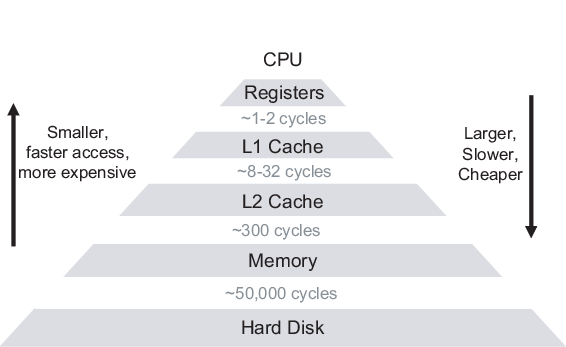
\includegraphics[width=0.6\textwidth]{figures/3_cpu/CPUherarchy.png}
	\caption{Hierarchy of memory types based on speed, cost, and capacity.}
\end{figure}

\subsubsection*{Cache Memory Operation}

% Explaining cache operation in detail
Cache memory operates on the principle of \textbf{locality}, which refers to the tendency of programs to access data and instructions that are close to each other in memory (spatial locality) or accessed repeatedly within a short time frame (temporal locality). The cache stores a subset of the main memory's contents in small, fast memory blocks called \textbf{cache lines}, typically 64 bytes in size. When the CPU requests data, the cache controller checks if the data resides in the cache. If it does (a \textbf{cache hit}), the data is retrieved quickly without accessing RAM. If it does not (a \textbf{cache miss}), the controller fetches the data from RAM or a lower-level cache, loading it into the cache for future access.

The cache is organized into \textbf{sets} and \textbf{ways}, forming an associative structure. For example, in a 4-way set-associative cache, each set can store four cache lines, and the cache controller uses a mapping function to determine which set a memory address corresponds to. If the target set is already full, the controller must evict a line (typically the least recently used) and repeated conflicts that keep evicting lines from the same set are known as \textbf{cache thrashing} \cite{CPUcachetrashing}.

\vspace{0.5em}

\begin{figure}[H]
	\centering
	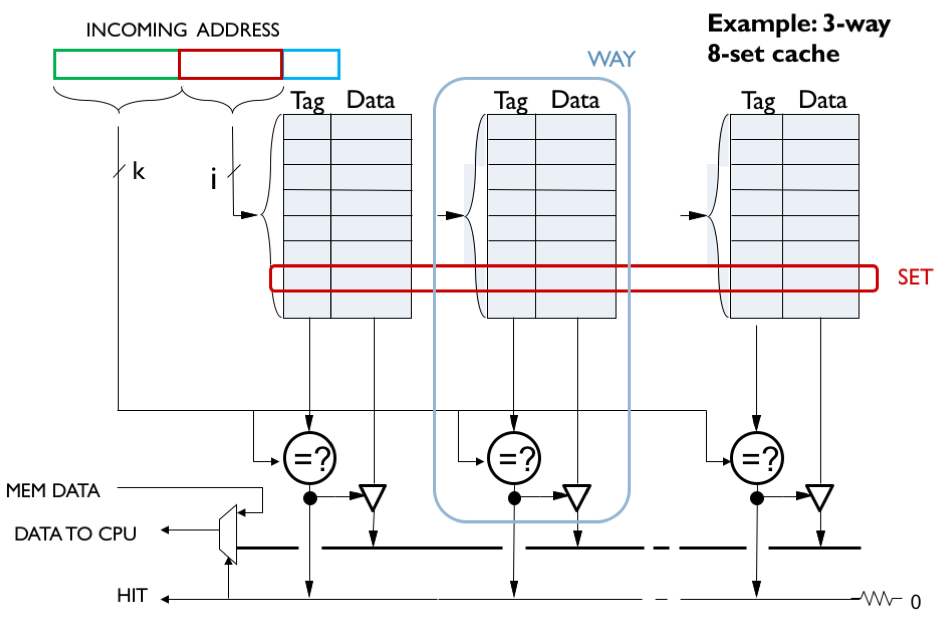
\includegraphics[width=0.75\textwidth]{figures/3_cpu/cache_ways_sets.png}
	\caption{\textbf{Set-associative cache (sets and ways).} Memory is cached in fixed-size lines (typically 64 B). When many cache addresses map to the same set and exceed the set's capacity, thrashing occurs. This organization explains why strided access patterns (e.g., row/column scans in matrices) can perform very differently depending on stride and problem size.}
\end{figure}

For now, we just need to understand the basic concepts of cache organization, including the roles of sets and ways, as well as the implications of cache hits and misses. But as we can see in the figure, this can be quite complex. Later sections will illustrate these concepts with practical examples.
\clearpage

\subsubsection*{RAM (Random Access Memory)}

\textbf{RAM} serves as the primary workspace for the CPU, storing data and program instructions that are actively in use. Unlike registers and cache, RAM offers significantly larger capacity (typically from 8GB to 64GB) but at the cost of much slower access speeds.

In an ideal scenario, the CPU retrieves the data it needs directly from its registers or from the cache, which are both extremely fast. However, if the required data is not present in any level of the cache hierarchy, a \textbf{cache miss} occurs. In this case, the CPU is forced to fetch the data from RAM, introducing a considerable delay in execution due to the higher memory latency.

This delay becomes particularly problematic in operations with low operation-to-data ratios, such as matrix-vector multiplication. As discussed in Chapter \ref{ch::chapter1}, Section\ref{subsec::operation_data_ratio}, MxV operations require frequent access to large portions of memory for relatively few computations, making them highly prone to cache misses. On the other hand, matrix-matrix multiplication (MxM) has a much higher operation-to-data ratio, allowing for better data reuse and more efficient use of the cache.

The performance of RAM is commonly described by two metrics: its \textbf{frequency} (in MHz), which affects memory bandwidth, and its \textbf{CAS latency} \cite{caslatency} (Column Access Strobe, or CL), which impacts memory access delay. CAS latency represents the number of clock cycles that elapse between the moment a memory controller sends a read command to a RAM module and when the data becomes available. However, since frequency determines how long each clock cycle lasts, the effective latency in nanoseconds is given by:

\[
\text{Latency (ns)} = \frac{\text{CL} \times 1000}{\text{Frequency (MHz)}}
\]

Hence, a higher frequency does not necessarily imply faster access unless CL is also considered. For instance, CL16 at 3200MHz results in a similar real latency to CL19 at 4000MHz:

\renewcommand{\arraystretch}{1.6}
\begin{table}[h!]
	\centering
	\begin{tabular}{|c|c|c|}
	\hline
	\textbf{Memory Speed} & \textbf{CAS Latency (CL)} & \textbf{Approx. Latency (ns)} \\ \hline
	3200 MHz             & CL16                      & $\frac{16 \times 1000}{3200} \approx 5$ ns \\ \hline
	4000 MHz             & CL19                      & $\frac{19 \times 1000}{4000} \approx 4.75$ ns \\ \hline
	2400 MHz             & CL17                      & $\frac{17 \times 1000}{2400} \approx 7.08$ ns \\ \hline
	\end{tabular}
	\caption{Estimated memory latency for different RAM configurations.}
\end{table}

Even newer memory technologies such as DDR5 aim to increase bandwidth and reduce latency through architectural improvements, such as dual or quad independent memory channels and higher burst lengths. However, the fundamental limitation of main memory remains: it is still significantly slower than L1, L2, or L3 cache, and orders of magnitude slower than registers.

\clearpage

\subsection{Cache Locality and Blocking}
\label{sec:cache_locality_and_blocking}

\textbf{Cache locality} refers to the efficient use of data elements that are either close together in memory (\textbf{spatial locality}) or accessed repeatedly in a short time frame (\textbf{temporal locality}). This aligns with how caches store data in 64-byte cache lines to minimize slower main memory access.

\textbf{Blocking} or tiling improves cache locality by dividing computations into smaller blocks that fit within cache, reducing cache misses and optimizing data reuse, especially beneficial for matrix multiplication. \cite{blocking}

In \textbf{Naive matrix multiplication}, each element $C(i,j)$ accesses entire row $A(i,*)$ and column $B(*,j)$. For large $N$, strided accesses (jumps of $N \times \text{element size}$ bytes) cause cache thrashing as data doesn't fit in cache and repeated accesses evict previously loaded cache lines.

\begin{figure}[H]
    \centering
    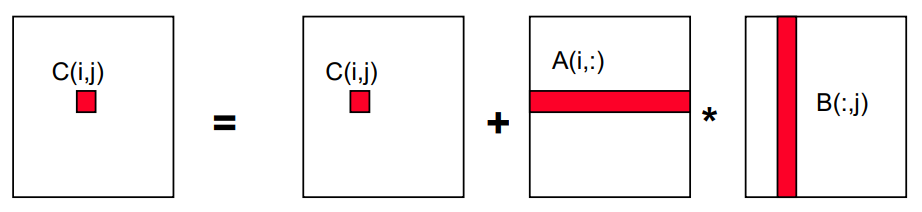
\includegraphics[width=0.9\textwidth]{figures/3_cpu/naiveMxM.png}
    \caption{Naive matrix multiplication algorithm.}
\end{figure}

\textbf{Blocked multiplication} partitions $A$, $B$, and $C$ into $b \times b$ blocks where $b$ fits in cache. For a 32KB L1 cache with FP32 elements, since three blocks must reside simultaneously:
\[
3b^2 \leq 8192 \quad \Rightarrow \quad b \leq \sqrt{\tfrac{8192}{3}} \approx 52
\]

The algorithm uses outer loops over blocks and inner loops for standard multiplication on each block, ensuring all necessary data resides in cache and leveraging both spatial and temporal locality.

\begin{figure}[H]
    \centering
    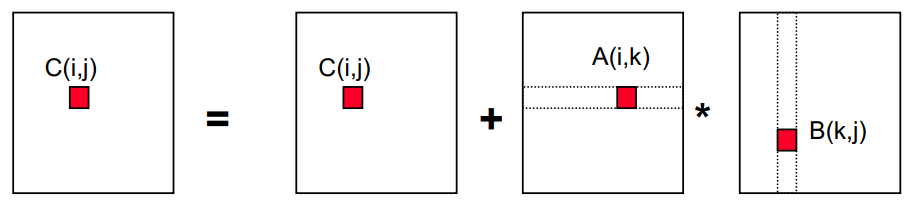
\includegraphics[width=0.9\textwidth]{figures/3_cpu/blockingMxM.png}
    \caption{Blocked matrix multiplication algorithm.}
\end{figure}

As mentioned in Chapter \ref{ch::chapter2}, blocking enables aggressive data reuse: tiles are reused $O(b)$ times, raising arithmetic intensity by factor $b$. Good blocking approaches the ideal $\tfrac{2}{3}N$ intensity, while naive approaches collapse to $O(1)$ due to repeated reloading. Libraries like BLAS and MKL implement these optimizations automatically.

\newpage

\section{Benchmarking on CPU}

In this section, we benchmark and compare the performance of \textbf{matrix–matrix multiplication} (MxM) and \textbf{matrix–vector multiplication} (MxV).  
The aim is to measure, for each operation, the sustained performance in $GFLOPS$ as the matrix size $N$ increases, and to contrast these measurements with theoretical limits imposed by both computation and memory access.

\vspace{0.5em}

\subsection*{Theoretical Compute Performance}

The theoretical time required to execute a given number of floating–point operations, assuming the CPU operates at its peak throughput, can be estimated as:
\begin{equation}
t_{CPU} = \frac{N_{ops}}{GFLOPS \times 10^9} \times 10^6,
\end{equation}

where $t_{CPU}$ is in microseconds. 

The peak performance in $GFLOPS$ is computed as:

\begin{equation}
GFLOPS = C_{CPU} \times CPU_{GHz} \times V_{vec} \times M_{ops}.
\end{equation}

\noindent The terms in the equation are:
\begin{itemize}
    \item $C_{CPU}$: number of \textbf{physical} CPU cores (logical threads are not counted here).
    \item $CPU_{GHz}$: CPU clock speed in GHz.
    \item $V_{vec}$: SIMD vector width in elements, which depends on the data type (e.g., single-precision 32-bit floats or double-precision 64-bit floats) and the instruction set architecture. The vector width $V_{vec}$ represents the number of elements that can be processed simultaneously in a single SIMD instruction. For example:
        \begin{itemize}
            \item Using \textbf{single-precision (F32, 32-bit)}:
                \begin{itemize}
                    \item AVX-512: $V_{vec} = 512 / 32 = 16$ elements per vector.
                    \item AVX2 (256-bit): $V_{vec} = 256 / 32 = 8$ elements per vector.
                \end{itemize}
            \item Using \textbf{double-precision (F64, 64-bit)}:
                \begin{itemize}
                    \item AVX-512: $V_{vec} = 512 / 64 = 8$ elements per vector.
                    \item AVX2 (256-bit): $V_{vec} = 256 / 64 = 4$ elements per vector.
                \end{itemize}
        \end{itemize}
    \item $M_{ops}$: floating–point operations per cycle per vector unit.
    For Fused Multiply–Add (FMA) \cite{FMA} instructions, each operation performs one multiplication and one addition in a single step, counting as two floating–point operations.
    For example, AVX2 \cite{AVX2} on the AMD Ryzen 5 5600X (Zen 3) can execute $2$ FMAs per cycle, resulting in $M_{ops} = 2 \times 2 = 4$.
\end{itemize}

\clearpage

\subsection*{Theoretical Memory Access Performance}

Even if the compute units can, in theory, reach a certain $GFLOPS$ peak, performance may be limited by memory bandwidth if it relies on it. This limitation arises because the rate at which data can be transferred to and from RAM often becomes a bottleneck, especially for memory-intensive operations such as matrix multiplications or large-scale vector computations. To estimate the time required to read or write the necessary data from/to RAM, we use a simplified model:

\begin{equation}
t_{mem} = \frac{N_{data}}{RAM_{Hz}} \times 10^6,
\end{equation}

where the terms are defined as follows:

\begin{itemize}
    \item $N_{data}$: the number of data elements that must be loaded from or stored into memory. This value depends on the specific operation being performed, such as the total number of elements in a matrix for matrix-matrix multiplication ($2 \cdot N^2$ for reading and writing) or the combined elements of a matrix and vector for matrix-vector multiplication ($N^2 + N$).
    \item $RAM_{Hz}$: the effective memory frequency in Hertz, which represents the clock rate at which the RAM operates. This frequency determines the maximum theoretical data transfer rate, assuming ideal conditions without overheads or inefficiencies.
\end{itemize}

This simplified model assumes that each clock cycle of the RAM can transfer one data element, and the time is converted to microseconds by multiplying by $10^6$.

However, it is important to note that this is a theoretical estimate and does not account for factors such as memory controller latency, bus contention, or the caches. For a more accurate estimation, one might consider the effective bandwidth and data size per element, but this model provides a baseline for understanding memory access costs.

For matrix-matrix multiplication (MxM), we estimate the real total memory access time by summing the individual measured components: the time to access a matrix by rows, the time to access a matrix by columns, and the time to allocate a matrix.

For matrix-vector multiplication (MxV), we sum the time to access a matrix by rows, the time to access a vector, and the time to allocate a vector.

\clearpage

\subsection{Benchmark Methodology}

The \textbf{GFLOPS benchmarks} are run using the \texttt{GFLOPS.jl} script where we do the following:
\begin{enumerate}
    \item Allocate:
    \begin{itemize}
        \item $A$: random $N \times N$ with \texttt{Float32} or \texttt{Float64} matrix.
        \item $B_{mat}$: random $N \times N$ with \texttt{Float32} or \texttt{Float64} matrix (for MxM).
        \item $B_{vec}$: random $N \times 1$ with \texttt{Float32} or \texttt{Float64} vector (for MxV).
    \end{itemize}
    \item Perform a \textbf{single multiplication} using \texttt{@benchmark} (\texttt{evals=1, samples=300}).
    \item Use the \textbf{minimum measured time} to approximate the sustained peak performance, reducing variability from noise and cache effects.
    \item Compute the sustained performance:
    \[
    GFLOPS_{\mathrm{MxM}} = \frac{2 N^3}{t_{MxM}} \times 10^{-9}, \quad
    GFLOPS_{\mathrm{MxV}} = \frac{2 N^2}{t_{MxV}} \times 10^{-9}.
    \]
\end{enumerate}

The \textbf{theoreticals memory access time $t_{mem}$ and compute time $t_{CPU}$ benchmarks} are run using the \texttt{tcpu\_tmemory.jl} and \texttt{tmemory.jl} scripts where we do the following:
\begin{enumerate}
    \item Compute the \textbf{theoretical times}:
    \begin{itemize}
        \item theoretical $t_{CPU}$: using the total number of floating-point operations for MxM or MxV, the peak $GFLOPS$ reported by \texttt{cpu\_info()} and the number of physical cores. To provide a realistic estimate, we utilize the base clock frequency rather than the turbo boost frequency.
        \item theoretical $t_{mem}$: using the number of data elements and the RAM frequency.
    \end{itemize}
    \item Measure the \textbf{measured execution times} for:
    \begin{itemize} % quiero poner aquí las llamadas de benchmark, ;a sí que no se repite el código
        \item measured $t_{CPU}$: using \texttt{@benchmark} on the matrix-matrix multiplication of $A$ and $B_{mat}$ and on the matrix-vector multiplication of $A$ and $B_{vec}$.
        \item measured $t_{mem}$: using \texttt{@benchmark} on the memory access patterns of the matrices and vectors. Includes row-wise and column-wise accesses, as well as vector accesses.
    \end{itemize}
\end{enumerate}

\vspace{1em}

\subsubsection*{Libraries and System (CPU, RAM)}

All benchmarks and plots are using MKL \cite{MKL} (BLAS/LAPACK) library. OpenBLAS was also tested but generally performed worse, especially for small matrices with MxM multi-core. 

The host system is an AMD Ryzen 5 5600X \cite{Ryzen5600Xspecs} (6C/12T) with a 3.7\,GHz base frequency (this base clock is used for the theoretical GFLOPS estimate) and 32\,GB DDR4 memory running at 3200\,MHz.


\clearpage

\subsection{Benchmark results: GFLOPS}
\label{sec:cpu_bench_results_GFLOPS}

This section reports CPU GFLOPS for dense matrix kernels and organizes the discussion around five ideas:
(A) single-core MxM vs.\ MxV, (B) multi-core MxM vs.\ MxV, (C) single \& multi MxM vs.\ theoretical peaks, (D) low-$N$ behavior (overheads vs.\ asymptotics), and (E) an overview for Float64.

In brief: on a single core, MxM consistently outperforms MxV; with multiple cores, MxM benefits markedly from parallelism while MxV remains bandwidth-bound; the single-core MxM curve tracks its theoretical limit closely, whereas the multi-core curve remains below its ideal due to shared-resource contention; at small sizes, parallel overheads can outweigh benefits; and Float64 sustains lower throughput but preserves the same qualitative behavior.

\subsubsection*{(A) FP32: Single-core \textnormal{MxM} vs.\ \textnormal{MxV}}
On a single core, matrix--matrix multiplication (MxM) delivers substantially higher GFLOPS than matrix--vector (MxV) across sizes. MxM is compute-bound with high arithmetic intensity ($O(N^3)$ work over $O(N^2)$ data), letting BLAS microkernels keep FMA pipelines busy and reuse cache-blocked tiles effectively. By contrast, MxV performs much less work per byte moved ($O(N^2)$ work over $O(N^2)$ data), so performance is limited by memory bandwidth and remains relatively flat with~$N$.

\begin{figure}[H]\centering
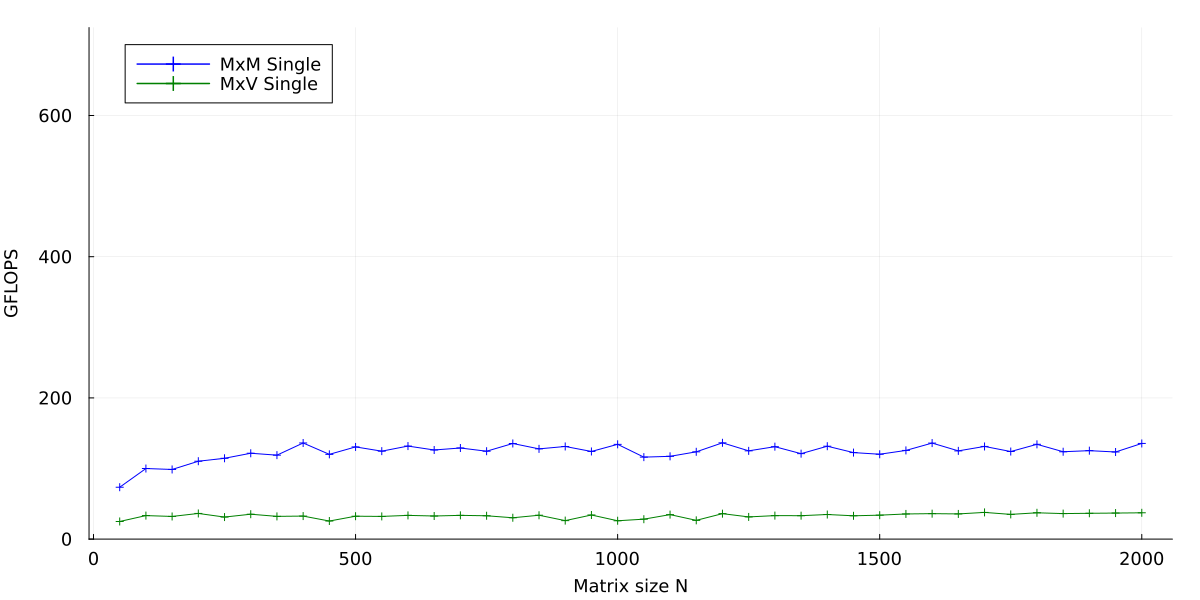
\includegraphics[width=\textwidth]{figures/3_cpu/gflops/Float32_GFLOPS_Ryzen5_5600X_MxM_vs_MxV_Single.png}
\caption{\textbf{FP32, single-core: MxM vs.\ MxV.} MxM clearly outperforms MxV across sizes. The reason is arithmetic intensity: MxM amortizes memory traffic via cache-blocked tiles and sustains high utilization of FMA units (compute-bound), whereas MxV quickly becomes limited by memory bandwidth (memory-bound), yielding a flatter, lower curve.}
\label{fig:cpu_gflops_fp32_single_mxm_mxv}
\end{figure}

\subsubsection*{(B) FP32: Multi-core \textnormal{MxM} vs.\ \textnormal{MxV}}
With multiple cores, MxM benefits strongly once $N$ is large enough for effective parallelism: the workload exposes ample independent blocks, and threading overheads become negligible relative to the total compute.

In contrast, MxV exhibits little separation between single-core and multi-core curves because additional cores share the same memory subsystem, so bandwidth remains the bottleneck.

\begin{figure}[H]\centering
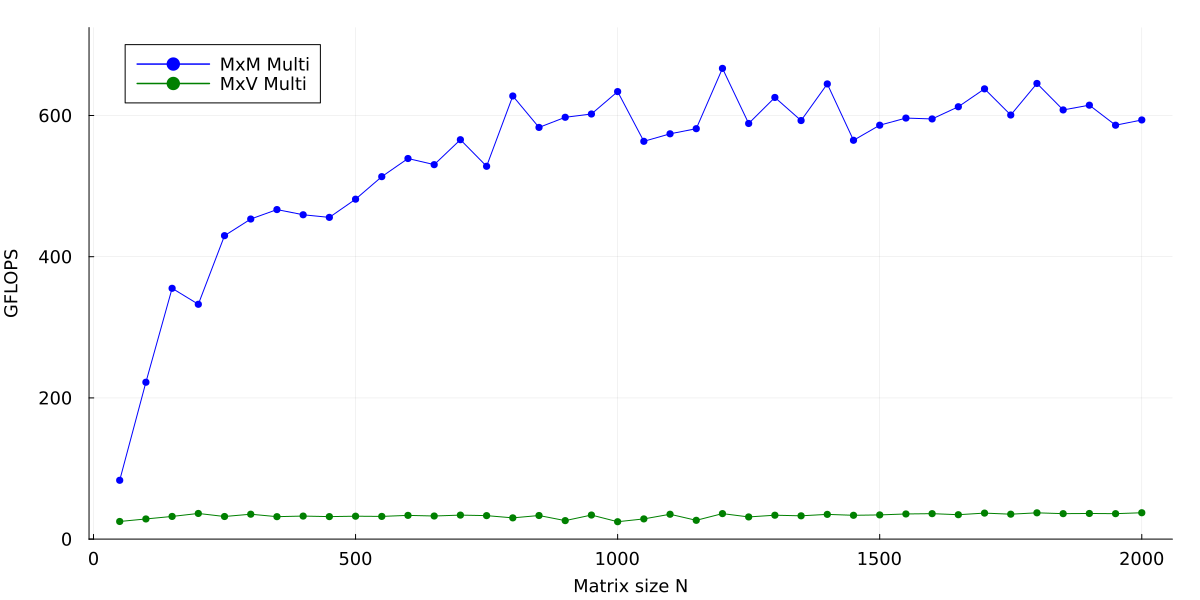
\includegraphics[width=\textwidth]{figures/3_cpu/gflops/Float32_GFLOPS_Ryzen5_5600X_MxM_vs_MxV_Multi.png}
\caption{\textbf{FP32, multi-core: MxM vs.\ MxV.} MxM gains markedly from parallelism once $N$ is sufficient to amortize threading overheads and feed all cores; MxV barely scales because RAM bandwidth is shared and already constraining performance, so extra cores cannot increase sustained FLOPS meaningfully.}
\label{fig:cpu_gflops_fp32_multi_mxm_mxv}
\end{figure}

Something to mention is that we see a slight drop for the largest $N$ near the end of the benchmark in MxM.

This behavior is typical under sustained all-core load: (i) power/thermal limits reduce all-core turbo frequencies (thermal or power throttling), and (ii) the working set exceeds the last-level cache, pushing more traffic to RAM because of cache misses.

\clearpage

\subsubsection*{(C) FP32: \textnormal{MxM} (single \& multi) vs.\ theoretical}
Comparing measured MxM to theoretical ceilings clarifies limits. The single-core curve typically tracks its peak closely because there is no inter-core contention and BLAS microkernels keep pipelines saturated with regular access patterns.

The multi-core curve, however, stays below its ideal due to lower all-core frequencies mostly because of power/thermal constraints, shared last-level cache and memory bandwidth.

\begin{figure}[H]\centering
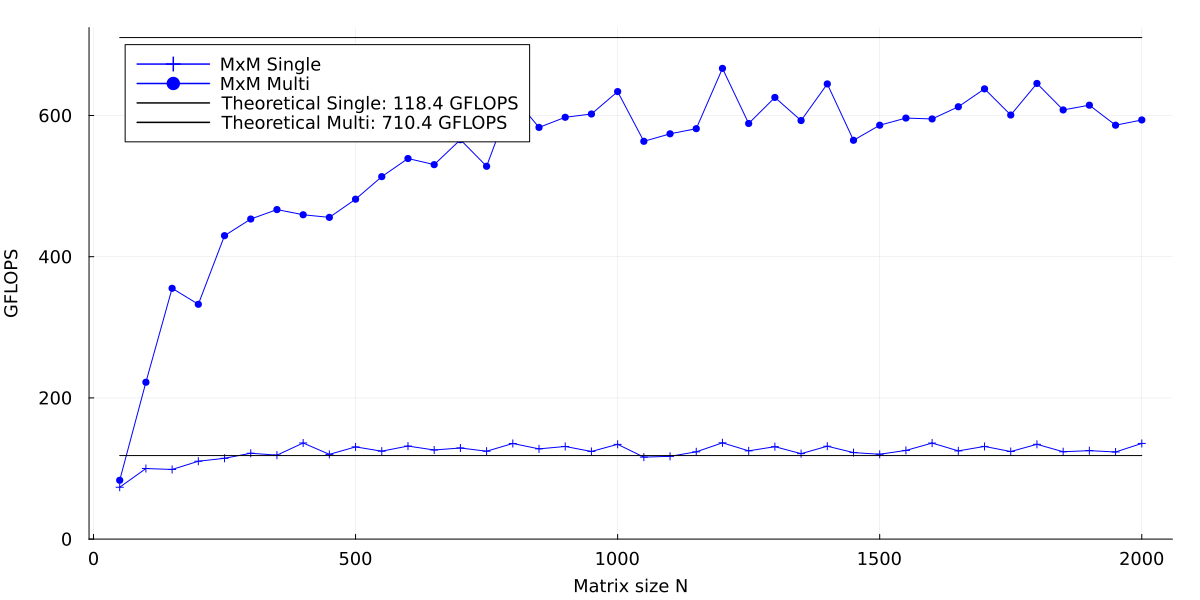
\includegraphics[width=\textwidth]{figures/3_cpu/gflops/Float32_GFLOPS_Ryzen5_5600X_MxM_Theo.png}
\caption{\textbf{FP32: MxM (single \& multi) vs.\ theoretical.} Single-core MxM exceeds the theoretical line thanks to efficient microkernel execution and no resource contention. Multi-core MxM rises with $N$ but remains below its theoretical bound because all-core turbo is lower than single-core boost and shared resources (shared L3 cache, memory bandwidth) and coordination overheads limit scaling.}
\label{fig:cpu_gflops_fp32_mxm_theoretical}
\end{figure}

It is important to note that the theoretical GFLOPS have been calculated by the script \texttt{system\_info.jl}, for the Ryzen 5 5600X, using the \textbf{base clock speed} and the number of cores. This is why the theoretical values are lower than the measured values in single core as they do not account for the boost clock speeds that are utilized during benchmarking when only a single core is active.

\clearpage

\subsubsection*{(D) FP32: Low-$N$ behavior (zoom)}
At small sizes, parallelization costs dominate: thread creation, synchronization, and less effective cache blocking can make multi-core performance match or even trail single-core. Those constant-time costs that are not negligible as at large $N$.

As $N$ grows, the asymptotic $O(N^3)$ compute of MxM quickly overwhelms overheads, tiles fit better into the blocking strategy, and multi-core scaling emerges toward its plateau.
\begin{figure}[H]\centering
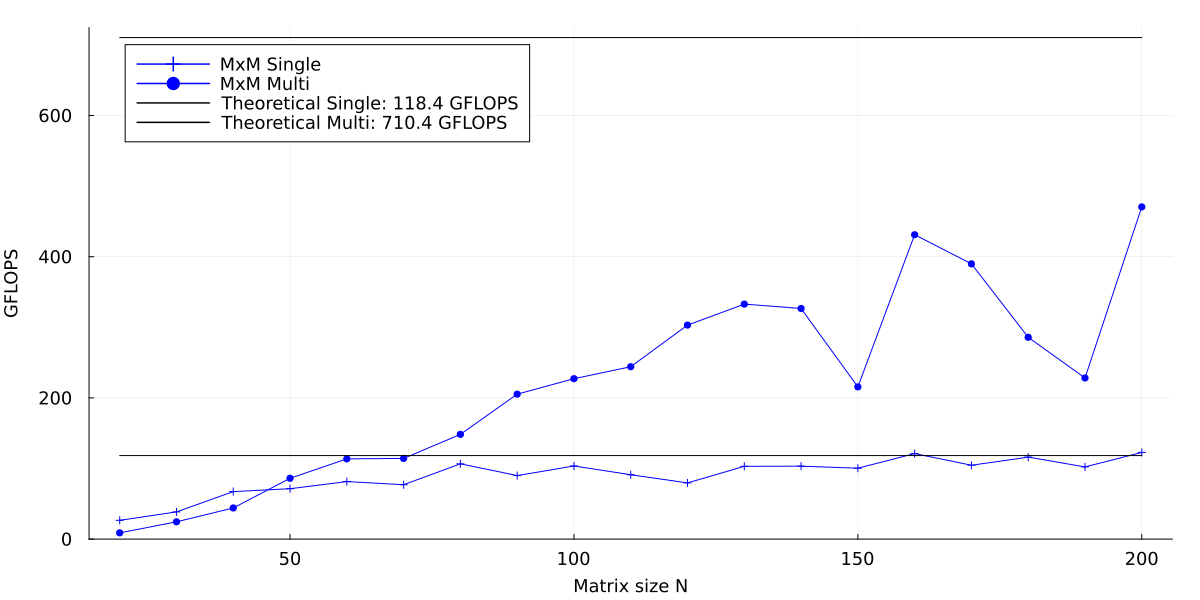
\includegraphics[width=\textwidth]{figures/3_cpu/gflops/Float32_GFLOPS_Ryzen5_5600X_MxM_Theo_lowN.png}
\caption{\textbf{FP32 (low-$N$ zoom): single vs.\ multi vs.\ theoretical for MxM.} For tiny matrices, multi-core can underperform due to overheads and limited reuse; single-core often benefits from excellent locality. Increasing $N$ restores the expected order: multi-core overtakes single-core as blocking becomes effective and parallel work dwarfs coordination costs.}
\label{fig:cpu_gflops_fp32_mxm_theoretical_lown}
\end{figure}

In practice, optimized libraries like MKL often employ dynamic threading (using few threads for small $N$, then increasing) precisely to avoid oversubscription in this regime, but this would not be as effective as using a single thread for very small $N$.


\clearpage

\subsubsection*{(E) Float64 (overview)}
With Float64, throughput drops relative to Float32 while preserving the same qualitative picture: MxM remains compute-bound and benefits from larger $N$ and multi-core parallelism, whereas MxV stays bandwidth-bound with minimal scaling.

The gap to multi-core theoretical peaks tends to widen because doubling the data size increases cache pressure and effective bandwidth demands per operation, accentuating shared-resource limits.

\begin{figure}[H]\centering
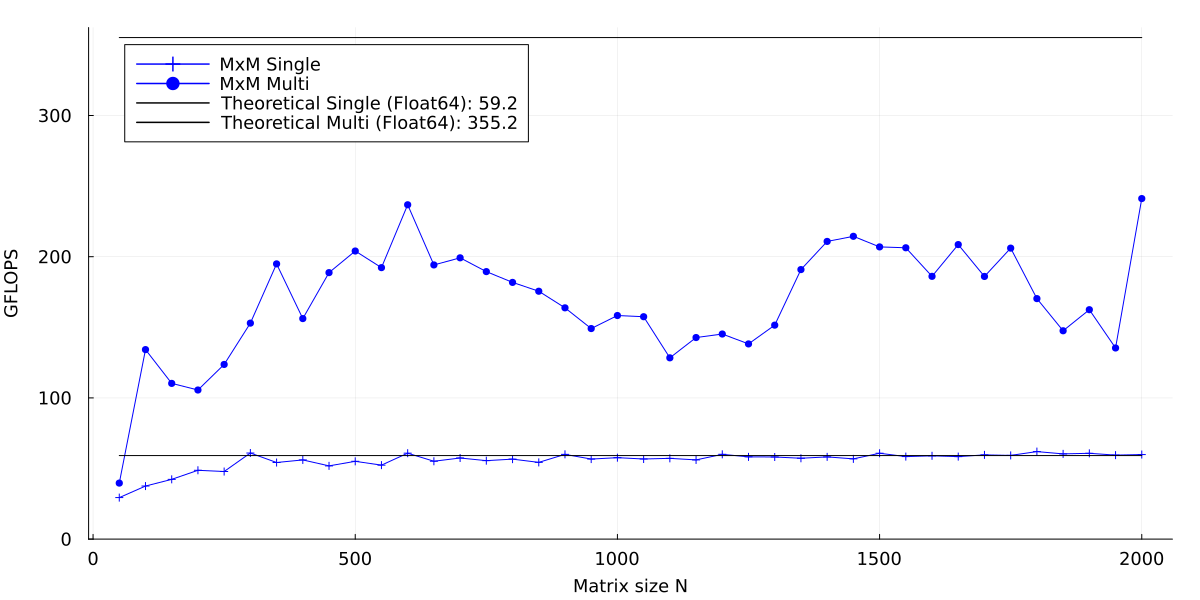
\includegraphics[width=\textwidth]{figures/3_cpu/gflops/Float64_GFLOPS_Ryzen5_5600X_MxM_Theo.png}
\caption{\textbf{FP64: MxM (single \& multi) vs.\ theoretical.} Same trends as FP32 with lower absolute throughput and a larger gap to the multi-core theoretical due to SIMD/FMA processing half as many elements per cycle and doubles consume twice the bytes and due to higher memory pressure and shared-resource contention}
\label{fig:cpu_gflops_fp64_mxm_theoretical}
\end{figure}

\textbf{y-axis scale warning:} When comparing FP64 and FP32 plots, be careful with the y-axis scale: FP64 theoretical peaks are roughly half of FP32 because a fixed-width SIMD register (e.g., AVX2 at 256 bits) holds half as many elements (4 doubles vs.\ 8 floats), halving FMA throughput per cycle. Additionally, as we already said, each element is twice the size, increasing memory pressure for bandwidth-bound kernels.


\clearpage

\subsection{Benchmark results: theoretical vs measured time}
\label{sec:cpu_bench_results_theoretical_vs_measured_time}

This section compares theoretical compute time ($t_{\text{CPU}}$) and theoretical memory time ($t_{\text{mem}}$) against measured execution times for MxM and MxV operations in a multi-core context.

The theoretical curves act as lower bounds: $t_{\text{CPU}}$ assumes perfect peak FLOPS utilization without stalls, while $t_{\text{mem}}$ assumes RAM-limited access without cache hierarchy benefits or overheads. Measured curves include those real effects.

\subsubsection*{(A) FP32: $t_{\text{CPU}}$ vs.\ $t_{\text{mem}}$ \textnormal{in MxM}}
For MxM, the operation-to-data ratio dominates the shape: the useful work grows as $O(N^3)$ while the moved data is $O(N^2)$. Consequently, $t_{\text{CPU}}$ grows faster with $N$ than $t_{\text{mem}}$. Optimized BLAS kernels (blocking/tiling) maximize reuse so the measured time follows the compute-bound trend and stays well above $t_{\text{mem}}$ for moderate and large $N$.

\begin{figure}[H]\centering
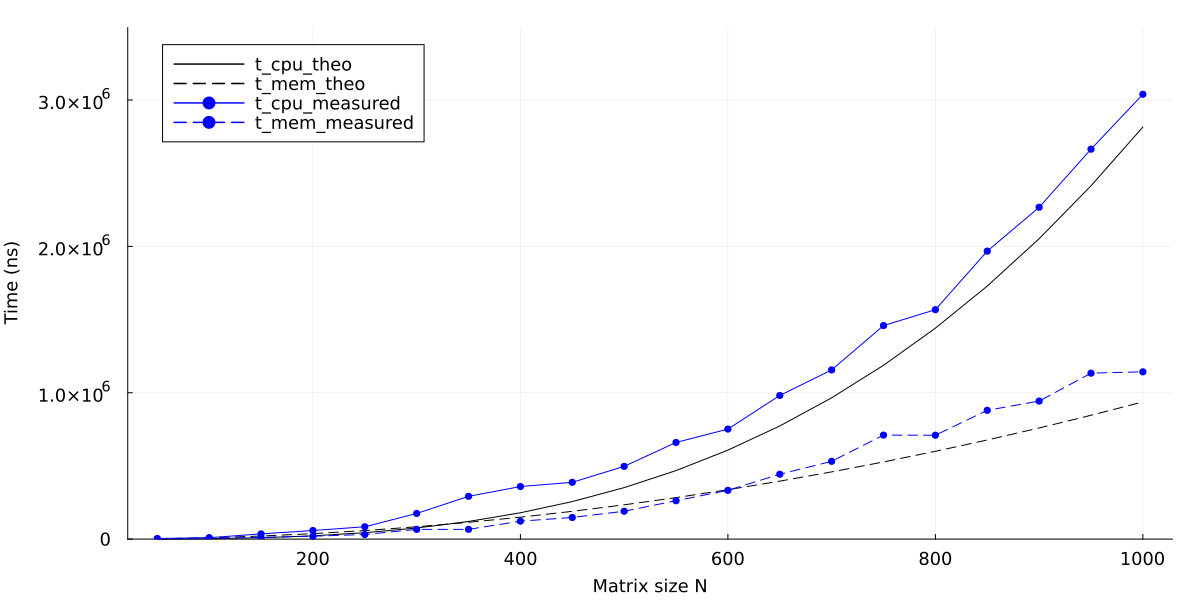
\includegraphics[width=\textwidth]{figures/3_cpu/tcpu_tmemory/Float32_MXM_Ryzen5_5600X.png}
\caption{\textbf{FP32 MxM: theoretical vs.\ measured times.} $t_{\text{CPU}}$ scales as $O(N^3)$ and dominates for moderate/large $N$; measured time tracks the compute-bound model thanks to cache-blocked reuse. $t_{\text{mem}}$ is a lower bound assuming RAM-limited traffic; real runs reuse data from caches and remain above it.}
\label{fig:tcpu_tmem_mxm_f32_full}
\end{figure}

Measured $t_{\text{mem}}$ is below the theoretical line across small and mid sizes (consistent with L1/L2/L3 reuse). A gentle crossover where measured $t_{\text{mem}}$ overtakes the RAM-only bound appears only near the upper end of the tested $N$ range, matching the expectation that cache capacity and controller saturation effects surface late in MxM due to strong reuse.

\clearpage

\subsubsection*{(B) FP32: $t_{\text{CPU}}$ vs.\ $t_{\text{mem}}$ \textnormal{in MxV}}
MxV has low arithmetic intensity ($O(N^2)$ FLOPs over $O(N^2)$ data) and quickly becomes bandwidth-bound. Here the theoretical $t_{\text{mem}}$ tends to dominate $t_{\text{CPU}}$.

For large $N$, the  memory time exceeds the theoretical bound due to cache misses, row/column conflict patterns and contention in the memory controller, none of which are modeled in the simple $t_{\text{mem}}$ bound.

\begin{figure}[H]\centering
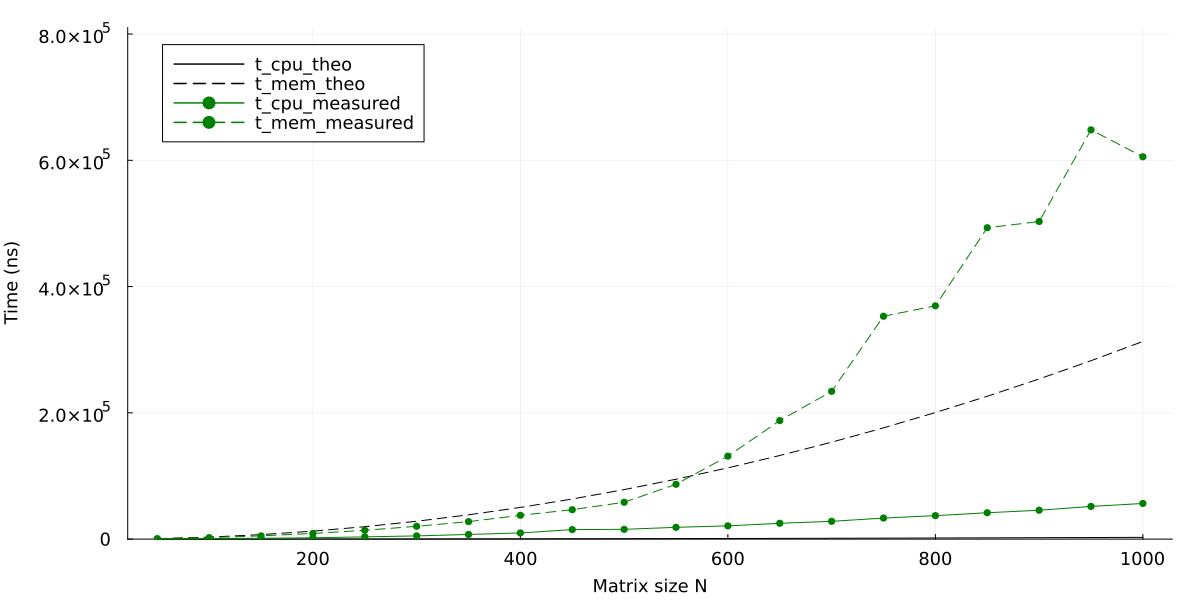
\includegraphics[width=\textwidth]{figures/3_cpu/tcpu_tmemory/Float32_MXV_Ryzen5_5600X.png}
\caption{\textbf{FP32 MxV: theoretical vs.\ measured times.} Bandwidth-bound across sizes: $t_{\text{mem}}$ dominates $t_{\text{CPU}}$. At large $N$, the measured memory time rises above the theoretical curve due to cache misses and controller saturation not captured by the simple RAM-bound model.}
\label{fig:tcpu_tmem_mxv_f32_full}
\end{figure}

The divergence (measured $t_{\text{mem}}$ climbing above the RAM-only line) appears already at mid-to-large sizes, earlier than in MxM and climbing faster due to the lower reuse in GEMV, which leads to increased memory pressure and contention. Keep in mind that the RAM-only bound is a simplified model that doesn't account for these overheads, causing the measured performance to be worse than predicted when cache efficiency degrades and memory subsystem bottlenecks emerge.

\clearpage

\subsubsection*{(C) FP32 (low-$N$ zoom): $t_{\text{CPU}}$ vs.\ $t_{\text{mem}}$ \textnormal{in MxM}}
With low-$N$, we see that the measured $t_{\text{CPU}}$ curve sits goes above what we expect, this is because of coordination costs multi-core overheads and short-run effects.

This can place the measured $t_{\text{CPU}}$ curve above the measured $t_{\text{mem}}$ initially, something that is maybe counterintuitive if we think that in these low-$N$ regimes, the impact of cache usage would help where all data fits in cache.

Those overheads can also be spotted in very low $N$ in the measured $t_{\text{mem}}$ curve, which can exceed the theoretical $t_{\text{mem}}$, because cache advantage does not overcome the increased coordination costs and multi-core overheads.

\begin{figure}[H]\centering
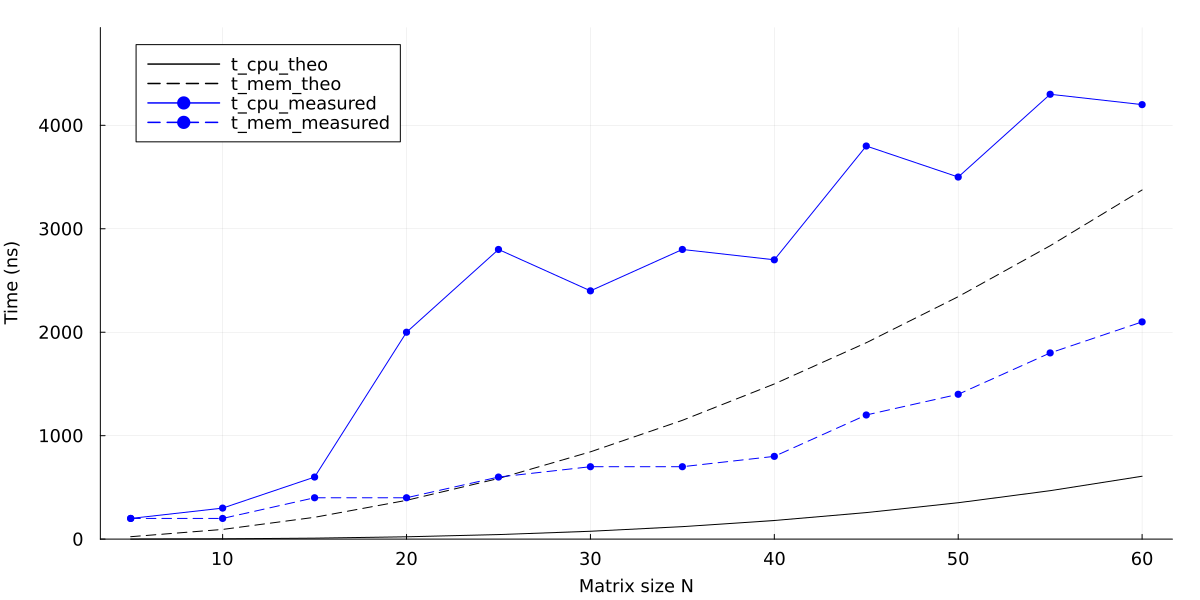
\includegraphics[width=\textwidth]{figures/3_cpu/tcpu_tmemory/Float32_MXM_Ryzen5_5600X_lowN.png}
\caption{\textbf{FP32 MxM (low-$N$ zoom):} In the low-$N$ regime, overheads can make measured $t_{\text{mem}}$ exceed the simple theoretical RAM-bound. The $t_{\text{CPU}}$ curve remains dominant as $N$ increases, reflecting the strong compute-bound nature of the operation.}
\label{fig:f32_mxm_60}
\end{figure}

Also, do not be misled if the theoretical $t_{\text{mem}}$ curve appears above the theoretical $t_{\text{CPU}}$ curve at tiny $N$ as the models scale differently. The theoretical $t_{\text{mem}}$ is quadratic in $N$ (e.g., $\sim 3N^2$ terms) while the theoretical $t_{\text{CPU}}$ is cubic (e.g., $\sim 2N^3$). For very small $N$, the quadratic with a larger constant sits above the cubic but as $N$ grows, the $N^3$ term inevitably dominates.

\clearpage

\subsubsection*{(D) \& (E) FP64: $t_{\text{CPU}}$ vs.\ $t_{\text{mem}}$ \textnormal{in MxM and MxV}}
In Float64, trends mirror FP32 but with larger data per element. Doubled bytes increase cache pressure and bandwidth demand, reflected in the $N$ at which measured $t_{\text{mem}}$ rises above the theoretical bound shifts to smaller sizes, reflecting earlier cache overflow.

\begin{figure}[H]\centering
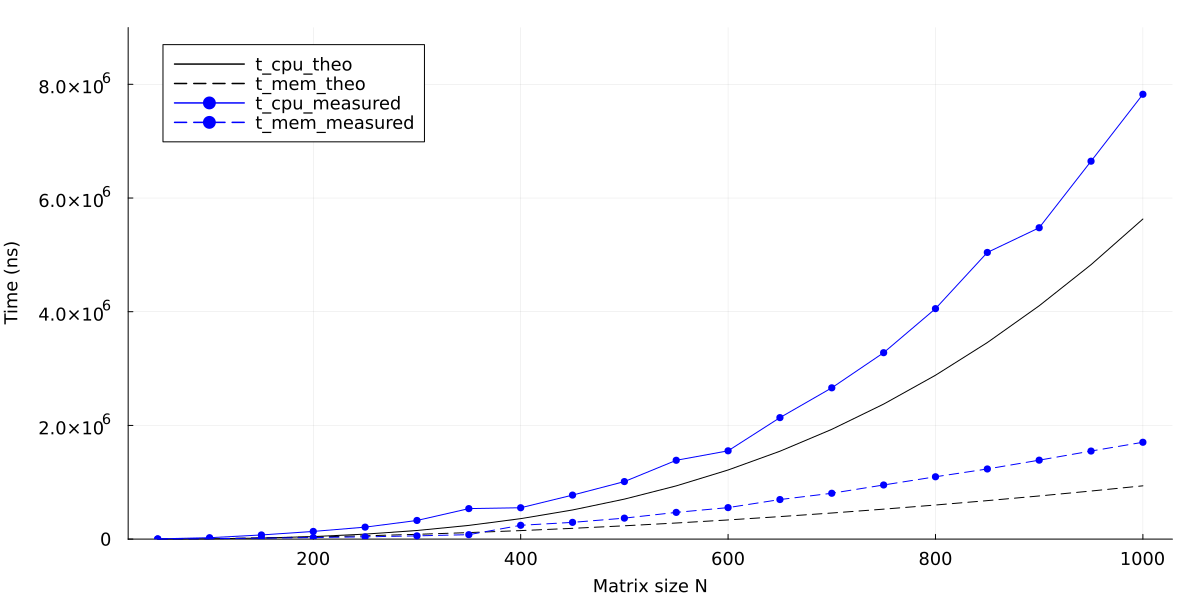
\includegraphics[width=\textwidth]{figures/3_cpu/tcpu_tmemory/Float64_MXM_Ryzen5_5600X.png}
\caption{\textbf{FP64 MxM: theoretical vs.\ measured times.} Same qualitative picture as FP32: compute-bound with measured times tracking $t_{\text{CPU}}$.}
\label{fig:tcpu_tmem_mxm_f64_full}
\end{figure}

\vspace{-1.5em}

\begin{figure}[H]\centering
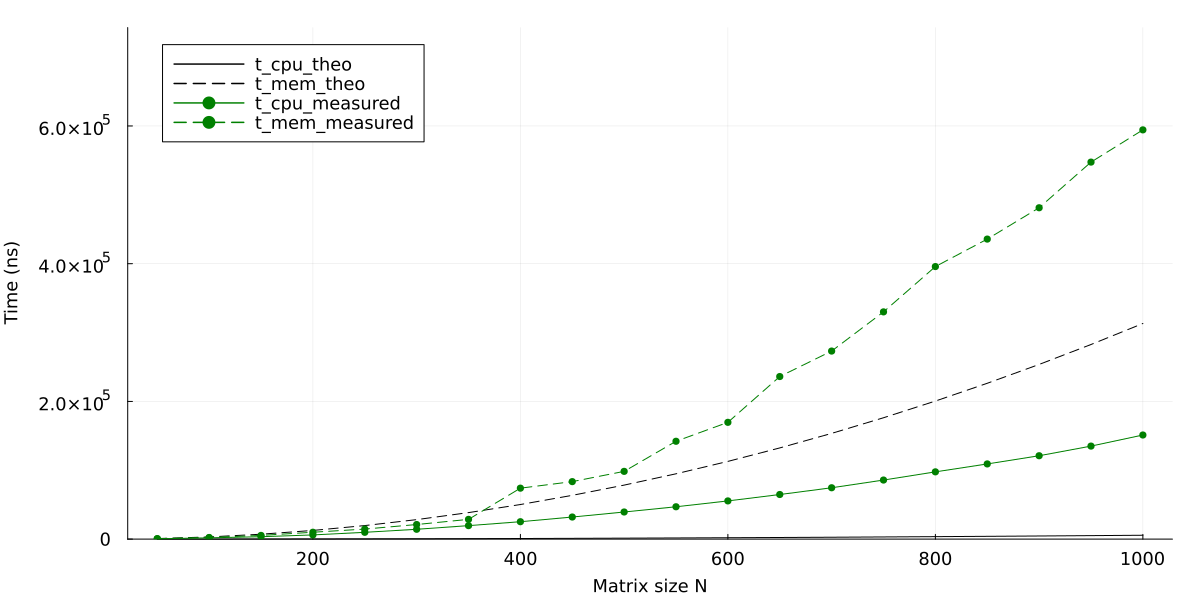
\includegraphics[width=\textwidth]{figures/3_cpu/tcpu_tmemory/Float64_MXV_Ryzen5_5600X.png}
\caption{\textbf{FP64 MxV: theoretical vs.\ measured times.} Even more bandwidth-bound than FP32: the crossover to measured $t_{\text{mem}}$ exceeding the theoretical bound occurs at smaller $N$ due to doubled element size and earlier cache overflow.}
\label{fig:tcpu_tmem_mxv_f64_full}
\end{figure}

\clearpage

\subsection{Benchmark results: cache conflict spikes}
\label{sec:cpu_bench_results_memory_conflict_spikes}

To expose cache–set conflicts explicitly, we rerun the memory-time experiment for \textbf{MxM} with a fine-grained grid of sizes \(N\) (step 8). We plot again the measured memory time for the kernel: the goal is to reveal conflict-driven spikes that can be masked by coarse sampling.

\subsubsection*{(A) FP32: conflict spikes with fine \(N\)}
In FP32, the memory-time curve shows pronounced spikes at regularly spaced sizes when scanning rows. In column-major layout, row-wise traversal advances by a stride of \(s=N\cdot \mathrm{sizeof}(\text{Float32})=4N\) bytes. With an L1 data cache of \(\,32\,\mathrm{KB}\), \(64\) sets, \(8\)-way associativity and \(64\)-byte lines, the set index advances by
\[
k \;=\; \frac{s}{64} \;=\; \frac{N}{16}\,.
\]
When \(k\) shares a large divisor with the \(64\) sets (e.g., \(N\) a multiple of \(128\)), accesses concentrate on few sets and saturate the \(8\)-way associativity, causing conflict misses and sharp latency spikes. Using a finer \(N\)-grid makes these resonances stand out clearly.

\begin{figure}[H]\centering
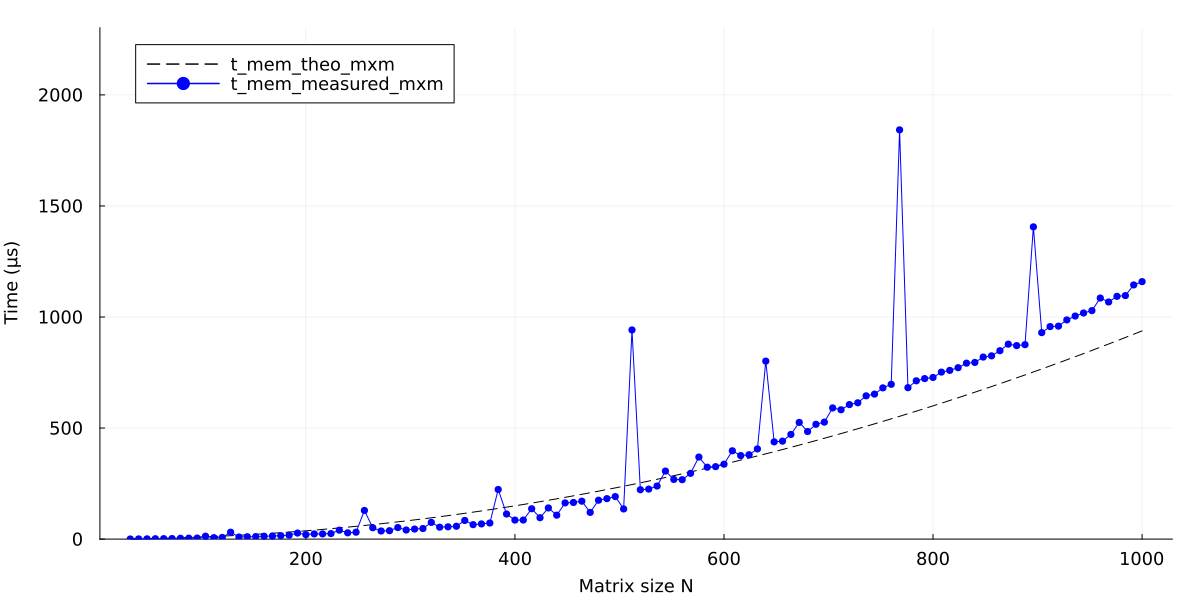
\includegraphics[width=0.95\textwidth]{figures/3_cpu/tmemory/Float32_MEMORY_MxM_Ryzen5_5600X.png}
\caption{\textbf{FP32 MxM (memory time, fine \(N\)).} Distinct spikes appear at conflict sizes where the row stride \(4N\) bytes aliases onto a small subset of the \(\,64\) L1 sets (32\,KB, 8-way, 64B lines). In those cases the set footprint exceeds the 8-way capacity and lines evict each other aggressively, inflating the measured memory time.}
\label{fig:mem_spikes_fp32}
\end{figure}

\vspace{-1em}

To understand the conflict spikes in an easier way, consider the following:

At \(N=128\), \(4N=512=64\times 8\): each column hop moves the cache set by exactly \(+8\), so you keep accessing the same 8 of 64 sets and overflow the 8-way associativity → spike.

At \(N=129\), \(4N=516=64\times 8+4\): that extra 4 bytes accumulates, so over time you visit all 64 sets and spread the pressure → no spike.

\clearpage

\subsubsection*{(B) FP64: same spikes plus interleaved ones}
In FP64, the same conflict sizes reappear and additional spikes emerge between them. The stride doubles to \(s=N\cdot \mathrm{sizeof}(\text{Float64})=8N\) bytes, so the set-step is
\[
k \;=\; \frac{s}{64} \;=\; \frac{N}{8}\,,
\]
which makes many more \(N\) satisfy the same aliasing condition (large \(\gcd(k,64)\)). As a result, conflict resonances occur more frequently (e.g., at multiples of \(64\), not only of \(128\)), producing interleaved spikes between the FP32 peaks. Moreover, each 64B line holds half as many elements (8 vs.\ 16), increasing pressure and amplifying spike height.

\begin{figure}[H]\centering
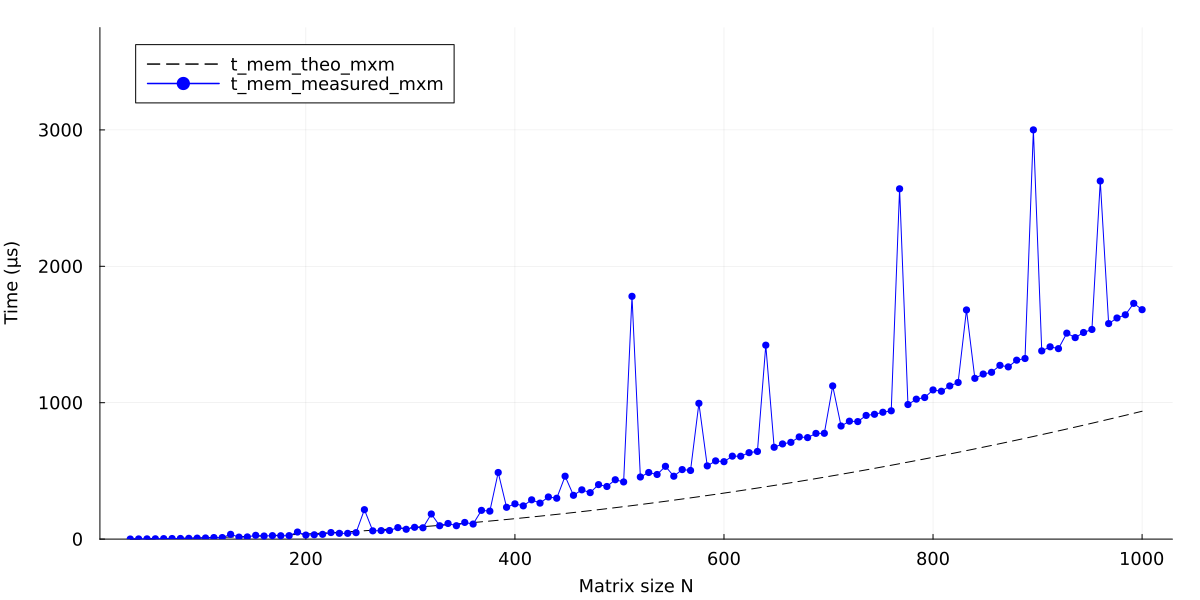
\includegraphics[width=0.95\textwidth]{figures/3_cpu/tmemory/Float64_MEMORY_MxM_Ryzen5_5600X.png}
\caption{\textbf{FP64 MxM (memory time, fine \(N\)).} The FP32 resonance sizes persist, and new interleaved spikes appear because the larger stride \(8N\) bytes increases the number of \(N\) that map onto few L1 sets (32\,KB, 64 sets, 8-way, 64B lines). With fewer doubles per line, conflict pressure is stronger and peaks are typically more pronounced.}
\label{fig:mem_spikes_fp64}
\end{figure}



% This file is included by main.tex

\chapter{GPU Architecture and Performance}
\label{ch::chapter4}

\vspace{-1cm}

\section{How a GPU Works}

\subsection*{Context and Relevance}
Having explored the significant capabilities of CPUs, particularly in handling complex sequential tasks, it is evident that they excel in low-latency operations and intricate control flows. However, when it comes to massive parallelization, GPUs emerge as the superior choice. Their architecture, specifically designed to execute thousands of simultaneous operations, makes them indispensable for tasks requiring extensive parallel processing.

In the last decade, Graphics Processing Units (GPUs) have evolved from being exclusive components for rendering graphics to becoming key tools in High-Performance Computing (HPC) \cite{GPUfundamentals}. Technologies such as artificial intelligence, physical simulations, data analysis, and scientific computing leverage the massive parallel architecture of GPUs, offering significant acceleration compared to Central Processing Units (CPUs).

\subsection*{Differences between CPUs and GPUs}
CPUs and GPUs have architectural designs optimized for different tasks:

\begin{itemize}
    \item \textbf{CPU (Central Processing Unit):}
    \begin{itemize}
        \item Designed to handle complex and sequential tasks.
        \item Contains few cores (typically on the order of 10-100) highly optimized for single-thread performance.
        \item Especially efficient for operations requiring low latency and complex control flows.
    \end{itemize}
    \item \textbf{GPU (Graphics Processing Unit):}
    \begin{itemize}
        \item Designed to execute a large number of operations in parallel.
        \item Contains hundreds or thousands of simpler cores organized in massively parallel processing blocks.
        \item Ideal for tasks with high parallelization, such as matrix multiplication and vector processing.
    \end{itemize}
\end{itemize}

\subsection{Host-Device Communication}
GPUs operate in conjunction with a CPU (host) through a well-defined communication topology. This topology involves two primary components:

\begin{itemize}
    \item \textbf{Host:} Refers to the CPU and its system memory (RAM).
    \item \textbf{Device:} Represents the GPU, including its on-board memories (global, shared, etc.).
\end{itemize}

\vspace{-1em}

\begin{figure}[H]
    \centering
    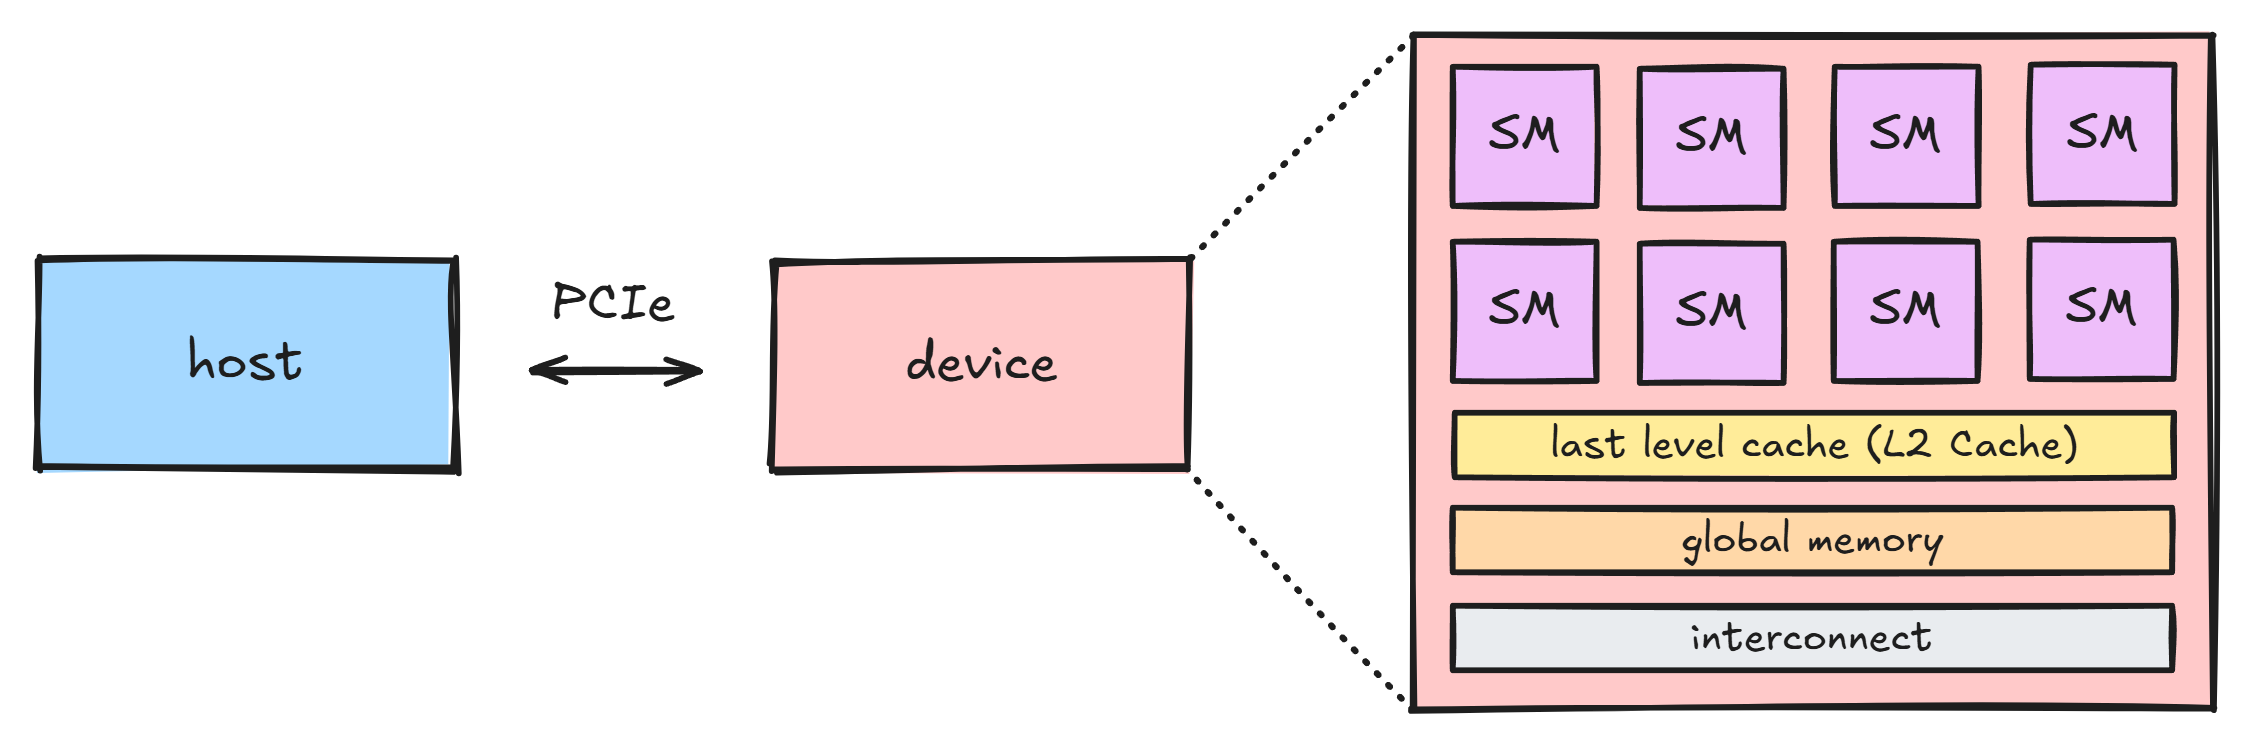
\includegraphics[width=0.8\textwidth]{figures/4_gpu/host_device_topology.png}
    \caption{Host-Device Communication Topology}
\end{figure}

\vspace{-0.5em}

This topology division is crucial as the code for launching the kernel and the data to be processed is also divided between a host function and a device function (kernel). The host is responsible for managing the data and launching the kernel, while the device executes the kernel in each thread and performs the computations.

A \textbf{kernel} \cite{GPUkerneloptimization,juliagpu} is a function that is executed by each thread in the GPU. The kernel must be written in a way that allows each thread to execute the same code but with different data. The host is responsible for launching the kernel to the GPU threads with the appropriate parameters and managing the data that will be processed by the kernel.

Before discussing the GPU itself, we need to understand that data transfer between the host and device occurs via the \textbf{PCI Express (PCIe) interface}.

\begin{table}[h]
    \centering
    \label{tab:pcie_bandwidth}
    \begin{tabular}{|c|c|c|c|c|}
        \hline
        \textbf{PCIe Version} & \textbf{Transfer Rate} & \textbf{x1 BW} & \textbf{x8 BW} & \textbf{x16 BW} \\
        \hline
        3.0 & 8 GT/s & 985 MB/s & 7.8 GB/s & 15.8 GB/s \\
        \hline
        4.0 & 16 GT/s & 1.97 GB/s & 15.8 GB/s & 31.5 GB/s \\
        \hline
        5.0 & 32 GT/s & 3.94 GB/s & 31.5 GB/s & 63 GB/s \\
        \hline
    \end{tabular}
    \caption{PCIe Bandwidth comparison for different versions.}
\end{table}

The NVIDIA GeForce RTX 3070 \cite{RTX3070specs} uses PCIe 4.0, achieving 31.5 GB/s maximum bandwidth for x16 connections. This typically isn't a bottleneck since data is usually transferred once at computation start and results returned at the end, but frequent host-device transfers could create bottlenecks.

\clearpage

\subsection{GPU Core Architecture and Memory}

The architecture of a GPU is designed to handle massive parallelization, with thousands of cores working simultaneously. The architecture is divided into several components, each with its own characteristics and functions.

\begin{figure}[H]
    \centering
    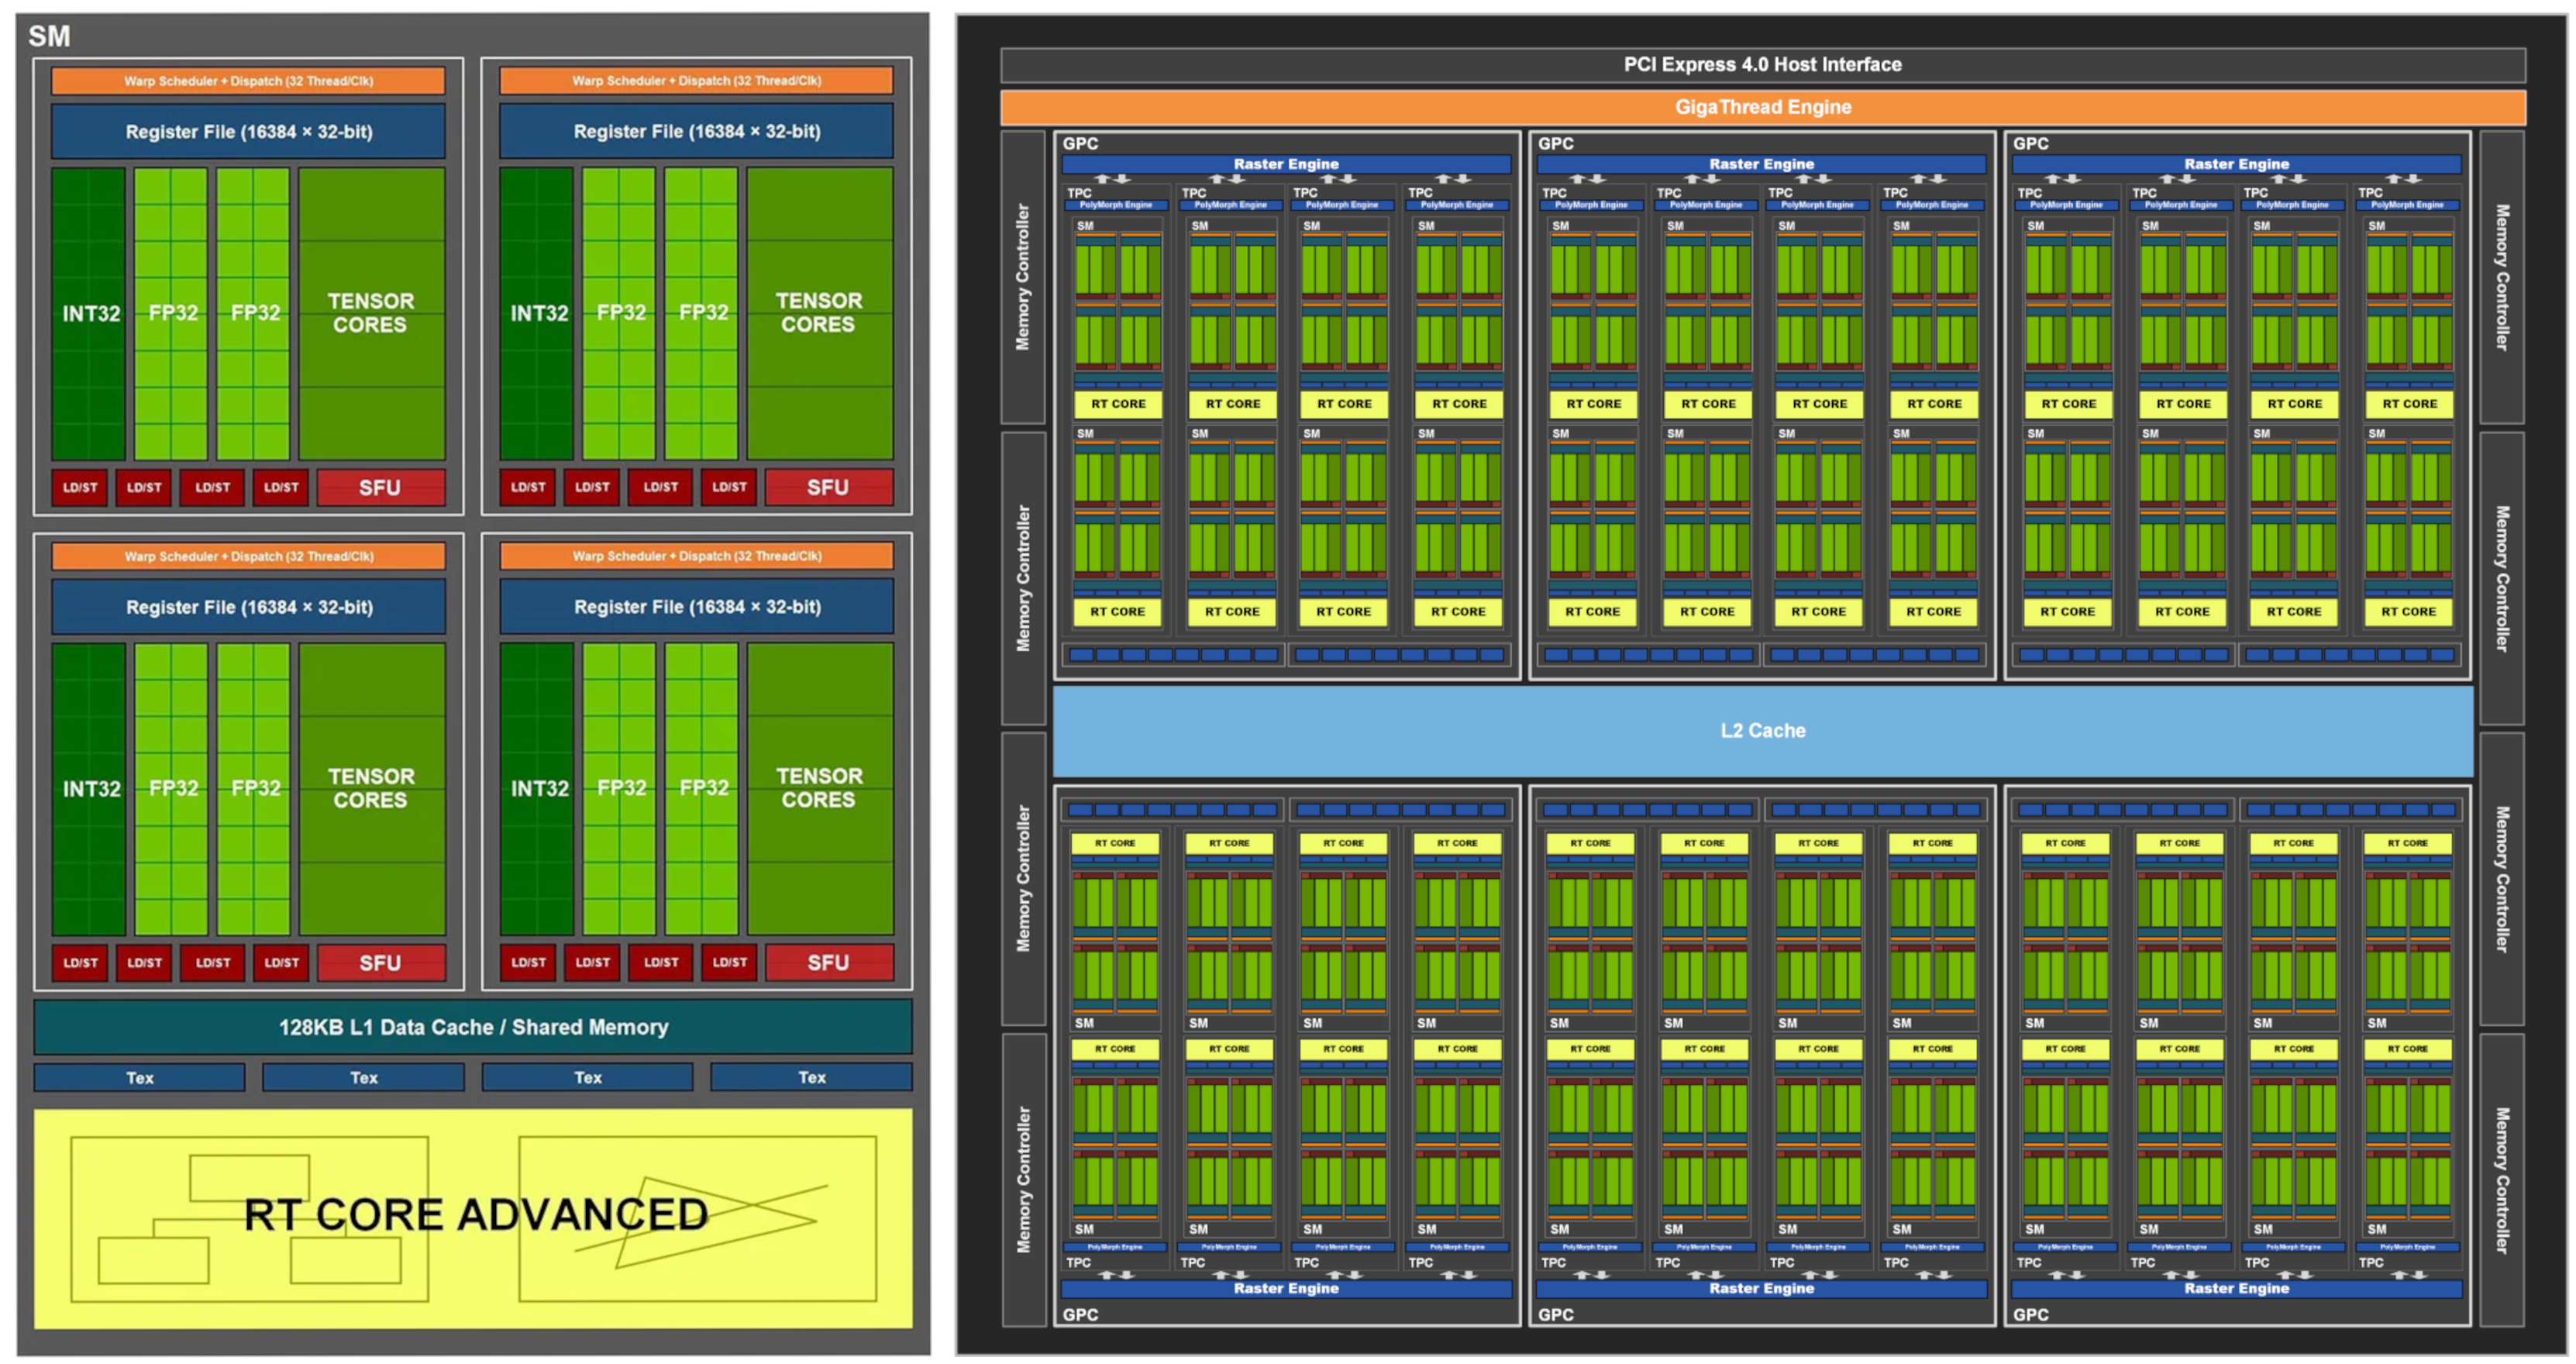
\includegraphics[height=8.5cm]{figures/4_gpu/GA104_Architecture.png}
    \caption{GA104 GPU (NVIDIA RTX 3070): Architecture and Streaming Multiprocessor}
\end{figure}

The GPU is divided into several Streaming Multiprocessors (SM), shown in the right image. AMD refers to these as Compute Units (CUs). Each SM contains several CUDA cores, which are the processing units of the GPU, responsible for executing threads in parallel. The CUDA cores are organized into warps, blocks, and grids \cite{GPUblocksandgrids}, which are the basic units of parallel execution in the GPU. This organization is explained in more detail in the next section.

The GPU architecture features a memory hierarchy divided into two regions \cite{GPUmemory}.

\textbf{On-Chip Memories (Per Streaming Multiprocessor):}
These provide high-speed access but with limited capacity.

\begin{itemize}
    \item \textbf{Registers:} The lowest-latency storage, integrated directly with the cores; organized into 32 banks (32 x 32-bit) corresponding to warp threads.
    \item \textbf{L1 Cache:} Serves as a buffer for register spills and frequently accessed data; physically unified with shared memory.
    \item \textbf{Shared Memory:} Explicitly managed by the programmer for intra-block data sharing; configurable partitioning with L1 cache.
    \item \textbf{Constant Caches:} Dedicated to read-only constants across threads in a warp or block.
\end{itemize}

\clearpage

\textbf{Off-Chip Memories (Shared Across Streaming Multiprocessors):}
These offer greater capacity at the expense of increased latency.

\begin{itemize}
    \item \textbf{L2 Cache:} A unified cache facilitating data transfer between global memory and PCIe.
    \item \textbf{Global Memory:} The primary device memory (e.g., GDDR6 on RTX 3070, bandwidth of approximately 500 GB/s); characterized by high latency (300--600 cycles).
    \item \textbf{Local Memory:} Utilized for register spill overflow beyond L1 and L2 caches; incurs significant performance penalties.
    \item \textbf{Texture and Constant Memory:} Optimized for specific access patterns, with texture data cached in L1 and constants in dedicated caches.
\end{itemize}

\subsubsection*{Memory Hierarchy}

The memory hierarchy in GPUs operates on principles of locality, both temporal (reusing data recently accessed) and spatial (accessing contiguous data), to minimize latency and maximize bandwidth in parallel workloads. When a thread requests data, the GPU traverses the hierarchy starting from the fastest, lowest-capacity levels closest to the cores, falling back to slower, higher-capacity levels only on misses.

\textbf{Data flow begins with registers}: if the required operand is in a thread's private registers, access is immediate (sub-cycle latency). \textbf{On a miss or overflow, the system checks the L1 cache} \cite{CPUcacheL1} (or shared memory for explicitly managed data), which may hit if the data was recently spilled or shared within the block. \textbf{Constant caches are consulted in parallel for read-only broadcasts}, optimizing uniform accesses across warps.

\textbf{If unresolved on-chip, the request propagates to the L2 cache} \cite{GPUcacheL2Global}, shared across SMs, which coalesces accesses from multiple warps and buffers global memory traffic. An L2 hit returns data in tens of cycles; \textbf{a miss triggers a fetch from global memory (DRAM)}.


\subsubsection*{Memory Locality}

Memory accesses in GPUs must be \textbf{coalesced} for efficiency: threads in a warp should access contiguous memory locations to minimize transactions. Non-coalesced accesses lead to serialized loads, wasting bandwidth.

In shared memory, \textbf{bank conflicts} occur when multiple threads access the same bank simultaneously, serializing accesses. Shared memory is divided into 32 banks (matching warp size), and proper padding or transposition can mitigate conflicts.

For global memory, alignment to 128-byte segments (cache line equivalent) is critical. In matrix operations, row-major versus column-major access patterns can cause uncoalesced loads, similar to CPU cache thrashing.

\subsubsection*{Tiling}

GPUs use \textbf{tiling} (also known as blocking in CPUs) to optimize performance by exploiting data locality. This technique involves loading small chunks of data, called tiles, from the slow global memory into the fast shared memory, where they can be reused multiple times by threads. This reduces the number of costly global memory accesses and increases \textbf{arithmetic intensity}, which measures the number of computations performed per byte of data transferred.

In a naive matrix multiplication, each thread computes one element of the result matrix \( C \), reading an entire row from matrix \( A \) and an entire column from matrix \( B \) from global memory. This leads to high memory traffic, roughly \( O(N^2) \) per thread, with low arithmetic intensity since few computations are done per data read. In contrast, tiling divides the matrices into smaller blocks, such as \( 32 \times 32 \) tiles, that fit in shared memory. Threads within a block work together to load these tiles, perform computations, and synchronize.

Libraries like \texttt{cuBLAS} and custom kernels apply \textbf{multi-level tiling}, using different tile sizes to optimize for shared memory, L1/L2 caches, and registers, depending on the GPU's architecture. For matrix-vector multiplication (MxV), however, tiling is less effective. Since each output element requires a full row of the matrix and the input vector with minimal data reuse, the operation has low arithmetic intensity (\( O(1) \)) and remains \textbf{bandwidth-bound}.

\subsection{Instruction-Level Parallelism: SIMT and Vectorization}

Modern GPUs employ a \textbf{Single Instruction, Multiple Threads (SIMT)} paradigm, analogous to SIMD in CPUs but scaled to thousands of threads. In SIMT, a single instruction is executed across multiple threads simultaneously, each operating on different data elements, making it highly efficient for data-parallel workloads like matrix operations.

Threads are grouped into \textbf{warps} (typically 32 threads on NVIDIA GPUs), executing the same instruction in lockstep. If threads in a warp diverge (e.g., due to conditional branching), the GPU serializes divergent paths, masking inactive threads, which can reduce efficiency. To maximize performance, kernels should minimize branch divergence.

FMA operations are critical in numerical workloads, counting as two floating-point operations per cycle. For matrix multiplication, high-level operations like GEMM are decomposed into tiled kernels that leverage SIMT parallelism and Tensor Cores for acceleration.

\clearpage

\section{Benchmarking on GPU}

In this section, we benchmark and compare the performance of \textbf{matrix–matrix multiplication} (MxM) and \textbf{matrix–vector multiplication} (MxV) on the GPU. The aim is to measure, for each operation, the sustained performance in $GFLOPS$ as the matrix size $N$ increases, and to contrast these measurements with theoretical limits imposed by both computation and memory access.

\vspace{0.5em}

\subsection*{Theoretical Compute Performance}

The theoretical time required to execute a given number of floating–point operations, assuming the GPU operates at its peak throughput, can be estimated as:

\begin{equation}
t_{GPU} = \frac{N_{ops}}{GFLOPS \times 10^9} \times 10^6,
\end{equation}

where $t_{GPU}$ is in microseconds.

The peak performance in $GFLOPS$ is computed as:

\begin{equation}
GFLOPS = C_{SM} \times C_{cores/SM} \times GPU_{GHz} \times M_{ops}.
\end{equation}

\noindent The terms in the equation are:
\begin{itemize}
    \item $C_{SM}$: number of Streaming Multiprocessors (e.g., 46 on RTX 3070).
    \item $C_{cores/SM}$: number of CUDA cores per SM (e.g., 128 on Ampere architecture).
    \item $GPU_{GHz}$: GPU clock speed in GHz (boost clock, e.g., 1.725 GHz on RTX 3070).
    \item $M_{ops}$: floating–point operations per cycle per core. For Fused Multiply–Add (FMA) instructions, each operation performs one multiplication and one addition in a single step, counting as two floating–point operations. On the NVIDIA RTX 3070 (Ampere), each CUDA core can execute 1 FMA per cycle, resulting in $M_{ops} = 2$.
\end{itemize}

This formula gives the peak for FP32 operations (e.g., 20.31 TFLOPS on RTX 3070). For FP64 in consumer GPUs, performance is typically limited intentionally (e.g., to 1/64 of FP32 on Ampere consumer cards, 317 GFLOPS) to encourage users needing high FP64 throughput to purchase more expensive HPC-oriented GPUs.

\clearpage

\subsection*{Theoretical Memory Access Performance}

Memory-bound operations are limited by global memory bandwidth or PCIe transfers. The time to access data is:

\begin{equation}
t_{mem} = \frac{N_{data} \times \text{Element Size}}{BW_{eff}} \times 10^6,
\end{equation}

where $BW_{eff}$ is the effective bandwidth and it is calculated dynamically from GPU attributes:

\begin{equation}
BW = 2 \times (f_{mem} \times 10^3) \times \frac{w_{bus}}{8},
\end{equation}

where:

\begin{itemize}
    \item $f_{mem}$ is the memory clock rate in kHz.
    \item $w_{bus}$ is the global memory bus width in bits.
    \item The factor $2$ accounts for double data rate (DDR) in GDDR memory.
    \item The $10^3$ converts kHz to Hz.
    \item Division by $8$ converts bits to bytes.
\end{itemize}

Both $f_{mem}$ and $w_{bus}$ can be obtained from the CUDA.jl package by running:

\begin{itemize}
    \item \texttt{CUDA.attribute(dev, CUDA.CU\_DEVICE\_ATTRIBUTE\_MEMORY\_CLOCK\_RATE)}
    \item \texttt{CUDA.attribute(dev, CUDA.CU\_DEVICE\_ATTRIBUTE\_GLOBAL\_MEMORY\_BUS\_WIDTH)}
\end{itemize}

This yields peak theoretical $BW$, e.g., $\approx 448 \times 10^9$ bytes/s (448 GB/s) on RTX 3070. 

For matrix-matrix multiplication (MxM), we estimate the real total memory access time by summing the individual measured components: the time to access a matrix by rows, the time to access a matrix by columns, and the time to allocate a matrix.

For matrix-vector multiplication (MxV), we sum the time to access a matrix by rows, the time to access a vector, and the time to allocate a vector.

\clearpage

\subsection{Benchmark Methodology}

The \textbf{GFLOPS benchmarks} are run using the \texttt{gflops\_1operation\_gpu.jl} script with CUDA.jl and cuBLAS. For each matrix size $N$, we do the following:
\begin{enumerate}
    \item Allocate random matrices/vectors on GPU: $A$ ($N \times N$), $B_{mat}$ ($N \times N$), $B_{vec}$ ($N \times 1$).
    \item Perform a warm-up multiplication to compile kernels.
    \item Benchmark a \textbf{single multiplication} using \texttt{@benchmark} (\texttt{evals=1}, 200 samples), taking the minimum time to compute sustained GFLOPS:
    \[
    GFLOPS_{\mathrm{MxM}} = \frac{2 N^3}{t_{MxM}} \times 10^{-9}, \quad GFLOPS_{\mathrm{MxV}} = \frac{2 N^2}{t_{MxV}} \times 10^{-9}.
    \]
\end{enumerate}

Theoretical peaks are derived from GPU specs via \texttt{gpu\_info()}. Benchmarks exclude host-device transfers to focus on pure device performance.

\textbf{Theoretical memory access time $t_{mem}$ and compute time $t_{GPU}$ benchmarks} are run using the \texttt{tgpu\_tmemory\_GPU.jl} script. For each matrix size $N$ we do:
\begin{enumerate}
    \item Compute the \textbf{theoretical times}:
    \begin{itemize}
        \item theoretical $t_{GPU}$: using the total number of floating-point operations for MxM or MxV and the peak $GFLOPS$ reported by \texttt{gpu\_info()} (based on SM count, clock, and FMA throughput, including the device FP32{:}FP64 ratio).
        \item theoretical $t_{mem}$: using the number of data elements to load/store and the GPU global memory bandwidth.
    \end{itemize}
    \item Measure the \textbf{measured execution times}:
    \begin{itemize}
        \item measured $t_{GPU}$: using \texttt{@benchmark} on $A \times B_{\text{mat}}$ (MxM, cuBLAS) and on $A \times B_{\text{vec}}$ (MxV, cuBLAS), device-only (excluding host–device transfers).
        \item measured $t_{mem}$: using \texttt{@benchmark} on memory access patterns over matrices and vectors (row-wise, column-wise, and vector) and on allocations, mirroring the CPU methodology.
    \end{itemize}
\end{enumerate}

\vspace{1em}

\subsubsection*{Libraries and System (GPU)}

All benchmarks and plots are using \texttt{CUDA.jl} and cuBLAS. 

The device is an NVIDIA GeForce RTX 3070 (Ampere, GA104) with 46 SMs and 8\,GB GDDR6 on a 256-bit bus (with an effective bandwidth of approximately 448\,GB/s).

Theoretical peaks are $\sim$20.3\,TFLOPS (FP32) and $\sim$317\,GFLOPS (FP64) (FP32{:}FP64 $\approx 64{:}1$).

\clearpage

\subsection{Benchmark results: GFLOPS}
\label{sec:gpu_bench_results_GFLOPS}

This section organizes the GPU GFLOPS discussion around three ideas:
(A) FP32 MxM vs.\ MxV, (B) FP32 MxM vs.\ FP64 MxM (hardware FP64 ratio), and (C) FP64 MxM vs.\ MxV. Throughout, we focus on trends rather than exact values.

\subsubsection*{(A) FP32: \textnormal{MxM} vs.\ \textnormal{MxV}}
On the RTX~3070, FP32 MxM ramps up quickly with $N$ and settles into a high plateau. This is the classic compute-bound behavior where cuBLAS tiling exploits shared memory and the L2 cache, keeping SM pipelines busy with high reuse.

In contrast, FP32 MxV stays far below, almost despreciable compared to MxM, and grows only modestly as $N$ increases. Its arithmetic intensity is tiny, so additional threads mostly wait on GDDR traffic rather than issuing more useful FMAs; performance is governed by memory bandwidth rather than by SM throughput.

\begin{figure}[H]\centering
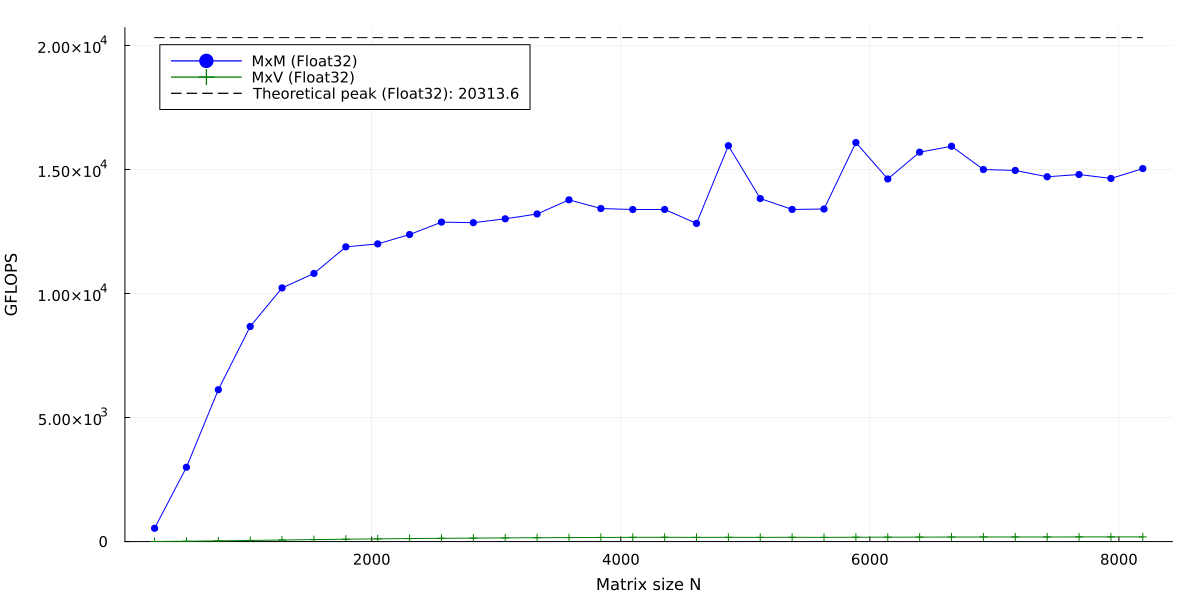
\includegraphics[width=\textwidth]{figures/4_gpu/gflops/FP32_GFLOPS_NVIDIA_GeForce_RTX_3070_MxM_vs_MxV.png}
\caption{\textbf{GFLOPS GPU FP32: MxM vs.\ MxV.} MxM, being compute-bound, climbs sharply and approaches a high plateau as cuBLAS tiles reuse data in shared memory and L2 cache. On the other hand, MxV, being memory-bound, sits much lower and changes little with $N$: extra parallelism cannot overcome the memory wall, so GFLOPS remain well below MxM.}
\label{fig:gpu_gflops_fp32_mxm_mxv}
\end{figure}

\noindent Minor undulations on the MxM curve at large $N$ are consistent with tile-size/occupancy boundaries and cache/L2 effects, but the overall picture remains a rise followed by a plateau.

\clearpage

\subsubsection*{(B) FP32 \textnormal{MxM} vs.\ FP64 \textnormal{MxM}}
Consumer Ampere GPUs throttle FP64 heavily (typically $\sim$1/64 of FP32 throughput). This is typically limited intentionally on consumer GPUs to encourage users needing high FP64 throughput to purchase more expensive HPC-oriented GPUs.

The result is that FP64 MxM reproduces the shape of the FP32 curve (tiling-driven ramp then plateau) but tops out at a much lower level, so cannot be even seen in the graph. This is fixed by a hardware ratio rather than by algorithmic limits. For large $N$, FP64 MxM consistently runs near its own (low) theoretical ceiling, illustrating that the bottleneck is architectural FP64 capacity, not inefficiency in the GEMM kernel.

\begin{figure}[H]\centering
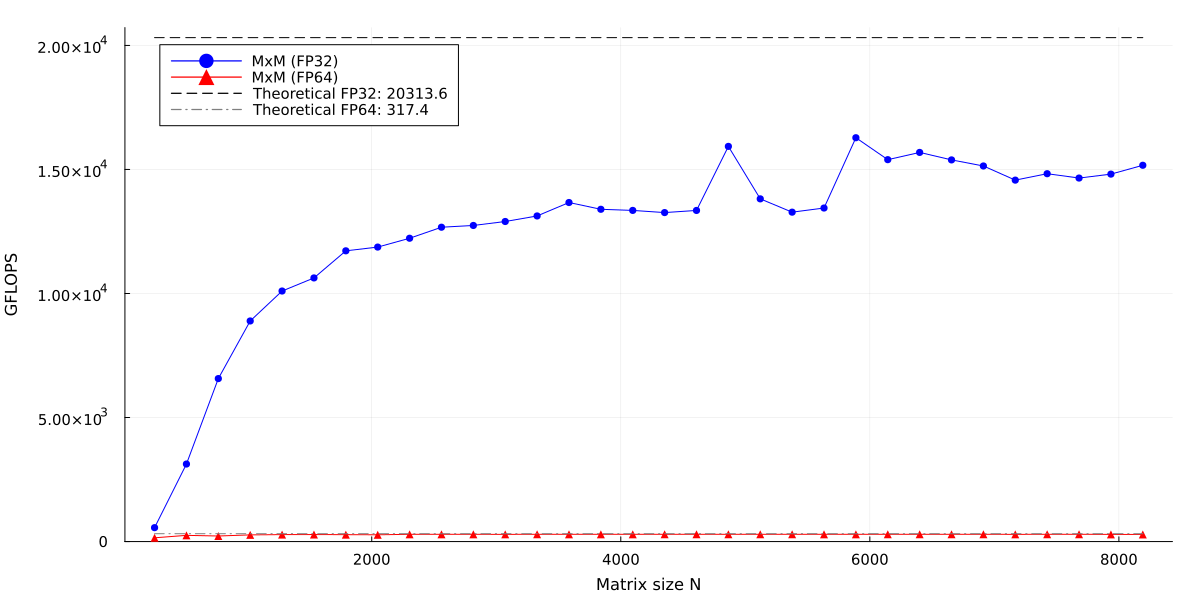
\includegraphics[width=\textwidth]{figures/4_gpu/gflops/FP32_vs_FP64_GFLOPS_NVIDIA_GeForce_RTX_3070_MxM.png}
\caption{\textbf{GFLOPS GPU: FP32 MxM vs.\ FP64 MxM.} Same scaling mechanics, different ceilings: FP64 saturates well below FP32 because consumer GPUs offer drastically reduced FP64 throughput. Large-$N$ FP64 MxM rides close to its own theoretical limit, highlighting a hardware cap rather than a software one.}
\label{fig:gpu_gflops_fp32_vs_fp64_mxm}
\end{figure}

The ratio between FP32 and FP64 units depends on the specific GPU architecture and its design choices.

For example, the NVIDIA RTX 3070 (Ampere consumer grade) has only 2 FP64 units per SM, while the NVIDIA A100 (a HPC grade oriented GPU) has 32 per SM.

\clearpage

\subsubsection*{(C) FP64: \textnormal{MxM} vs.\ \textnormal{MxV}}
With FP64, the MxM curve is compute-capped by the architecture as we commented earlier, and MxV remains bandwidth-bound. However, the GPU’s memory system is fast (the GPU NVIDIA RTX 3070 memory bandwidth is approximately 448 GB/s while the CPU’s is around 50 GB/s on DDR4 Dual Channel 3200 MHz).

Consequently, FP64 MxV climbs to a sizable fraction of FP64 MxM at large $N$ (much closer, in relative terms, than in FP32).

In other words, even though FP64 compute is throttled, the high GDDR bandwidth of the GPU lets a memory-bound kernel exploit a larger share of the available “budget” (the higher memory bandwidth) than it ever could on CPU RAM.

This is why FP64 MxV looks against FP32, comparatively healthy on the GPU, as the faster memory system provides a significant advantage.

\begin{figure}[H]\centering
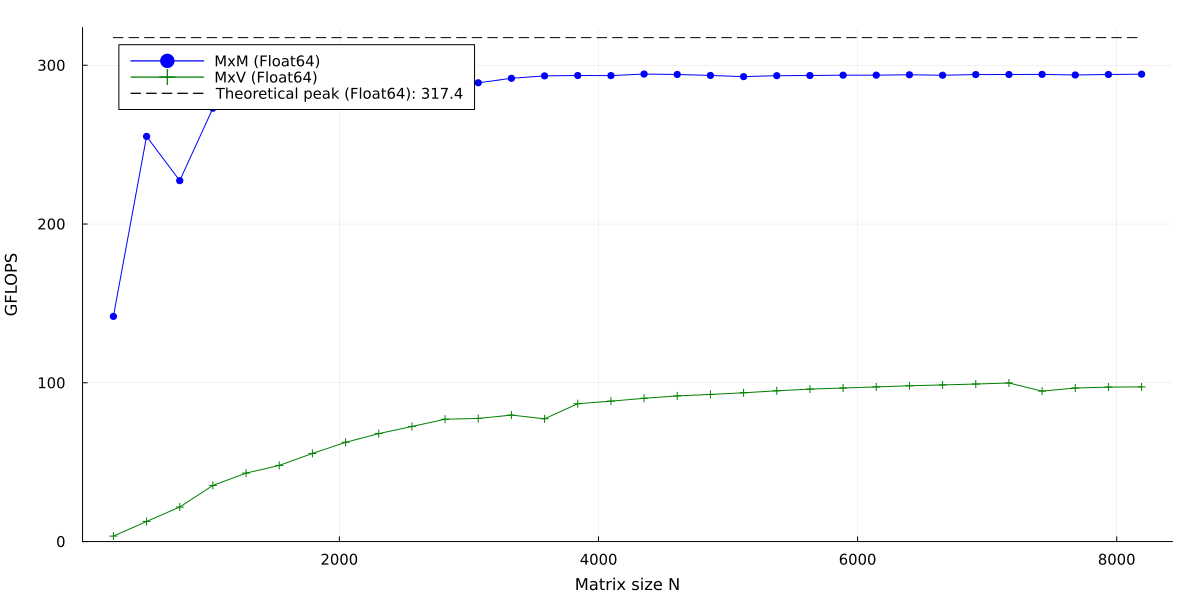
\includegraphics[width=\textwidth]{figures/4_gpu/gflops/FP64_GFLOPS_NVIDIA_GeForce_RTX_3070_MxM_vs_MxV.png}
\caption{\textbf{GFLOPS GPU FP64: MxM vs.\ MxV.} FP64 compute is heavily throttled, but memory bandwidth is unchanged. As a result, FP64 \textbf{MxV} (bandwidth-bound) reaches a substantial fraction of FP64 \textbf{MxM}, shrinking the relative gap vs.\ FP32. This underscores that the limiter for MxV is memory, where GPUs enjoy a big advantage over CPUs.}
\label{fig:gpu_gflops_fp64_mxm_mxv}
\end{figure}

Finally, in both precisions you may notice lower GFLOPS at very small $N$, where those points are dominated by fixed kernel-launch and setup overheads before the workload is large enough to amortize them.

\clearpage

\subsection{Benchmark results: theoretical vs measured time}
\label{sec:gpu_bench_results_theoretical_vs_measured_time}

We compare theoretical GPU compute time ($t_{\text{GPU}}$) and theoretical memory time ($t_{\text{mem}}$) to measured times. As with CPUs, $t_{\text{GPU}}$ is a compute-bound lower bound (ideal SM utilization), and $t_{\text{mem}}$ is a bandwidth-bound lower bound (ideal coalescing, no overheads).

\subsubsection*{(A) FP32: $t_{\text{GPU}}$ vs.\ $t_{\text{mem}}$ in \textnormal{MxM}}
For FP32 \textbf{MxM}, the operation-to-data ratio dominates again: $O(N^3)$ work over $O(N^2)$ data. cuBLAS’s tiling packs blocks into shared memory, driving reuse and keeping warps busy; measured times follow $t_{\text{GPU}}$ closely and stay well above $t_{\text{mem}}$ for moderate/large $N$.

\begin{figure}[H]\centering
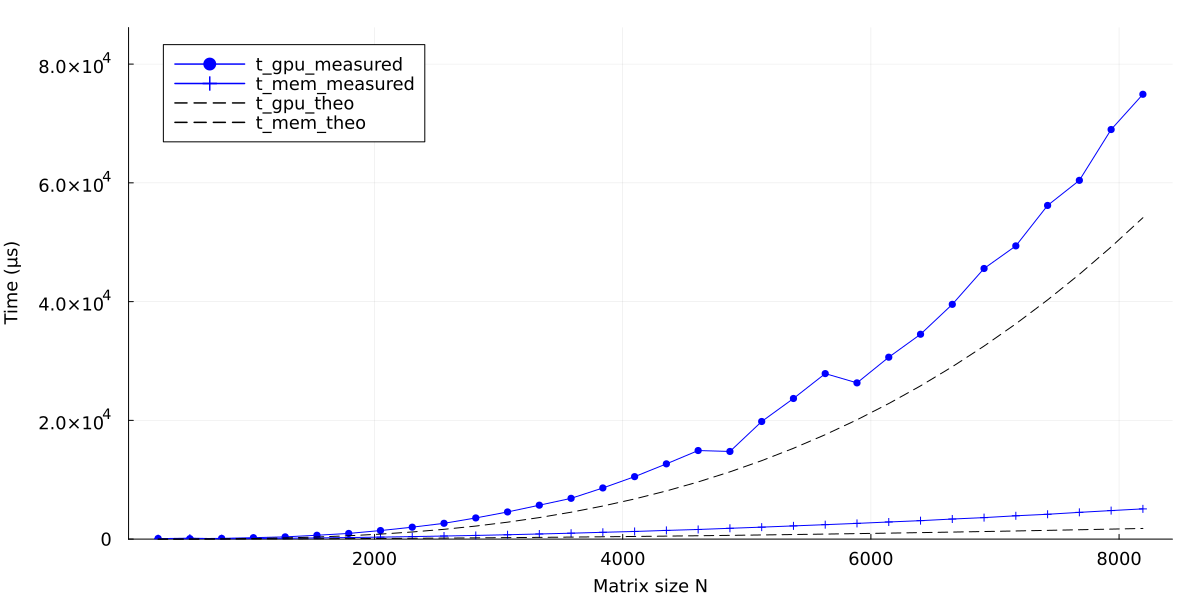
\includegraphics[width=\textwidth]{figures/4_gpu/tgpu_tmemory/Float32_MXM_NVIDIA_GeForce_RTX_3070.png}
\caption{\textbf{GPU FP32 MxM: theoretical vs.\ measured times.} Compute-bound: measured \(t_{\text{GPU}}\) tracks the theoretical \(t_{\text{GPU}}\) as tiling and reuse sustain high SM occupancy; \(t_{\text{mem}}\) remains a lower bound that is not reached in practice. The \(O(N^3)\) vs.\ \(O(N^2)\) scaling widens the gap with $N$.}
\label{fig:gpu_tgpu_tmem_fp32_mxm}
\end{figure}

We can observe that the measured time is consistently above the theoretical compute time, which is expected due to overheads and inefficiencies. However, the gap does not widen dramatically with $N$ because the kernel remains compute-bound, and cuBLAS optimizations keep the GPU busy.

\clearpage

\subsubsection*{(B) FP32 (low-$N$ zoom): kernel-launch overheads}
At small sizes, fixed costs dominate (kernel launch latency, queueing, synchronization, initializations). Both measured curves sit far above their theoretical bounds: there is simply too little work to amortize the launch.

\begin{figure}[H]\centering
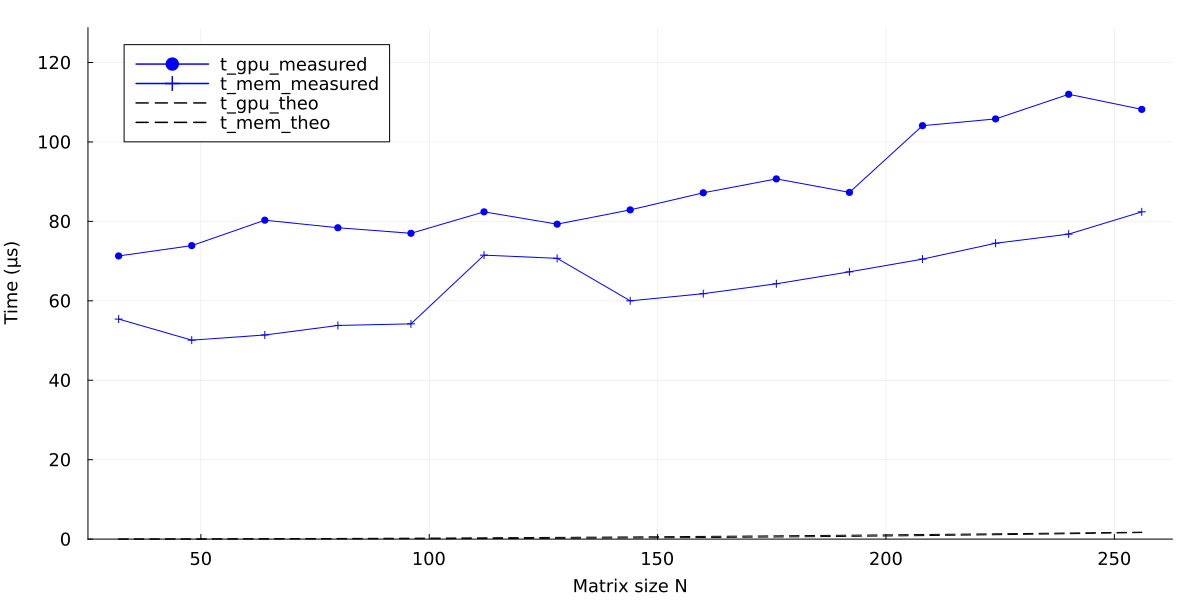
\includegraphics[width=\textwidth]{figures/4_gpu/tgpu_tmemory/Float32_MXM_NVIDIA_GeForce_RTX_3070_lowN.png}
\caption{\textbf{GPU FP32 MxM (low-$N$ zoom):} Measured times \(\gg\) theoretical bounds due to launch/scheduling overheads and underutilization of SMs at tiny problem sizes. Past a threshold $N$, overheads are amortized and the curve collapses toward the compute-bound regime.}
\label{fig:gpu_tgpu_tmem_fp32_mxm_lown}
\end{figure}

Concretely, at $N{=}32$ the theoretical times are essentially negligible (\(t_{\text{GPU}}\!\approx 0\,\mu\mathrm{s}\), \(t_{\text{mem}}\!\approx 0\,\mu\mathrm{s}\)), while the measurements are around the \(80\,\mu\mathrm{s}\) mark.

Even at $N{=}256$, the theoretical \(t_{\text{GPU}}\) does not match the measured \(t_{\text{GPU}}\!\approx 100\,\mu\mathrm{s}\). These gaps are the fixed launch/setup costs being amortized too slowly at small problem sizes.

This is due to the host-device model: the CPU must launch the kernel and manage data transfers, which adds latency that is significant when the workload is small.

\clearpage

\subsubsection*{(C) FP64: $t_{\text{GPU}}$ vs.\ $t_{\text{mem}}$ in \textnormal{MxM}}
In FP64 MxM the operation-to-data ratio still rules: $2N^3$ FLOPs vs.\ $\mathcal{O}(N^2)$ bytes.

However, as consumer GPUs throttle FP64 throughput (e.g., $\sim$1/32–1/64 of FP32), the kernel is even more compute-bound. As we see at the y-axis scale, the measured $t_{\text{GPU}}$ reaches two orders above that we had in FP32.

Again, $t_{\text{mem}}$ remains well below compute time despite doubling the element size (8\,B) relative to FP32.

\begin{figure}[H]\centering
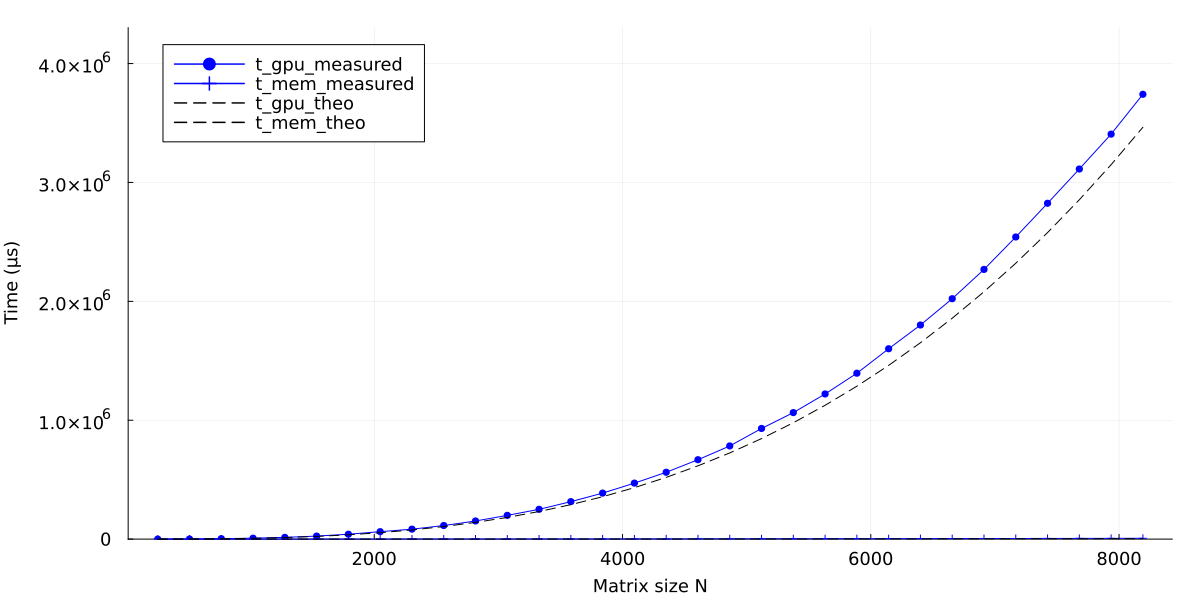
\includegraphics[width=\textwidth]{figures/4_gpu/tgpu_tmemory/Float64_MXM_NVIDIA_GeForce_RTX_3070.png}
\caption{\textbf{GPU FP64 MxM: theoretical vs.\ measured times.} Same $N^3$ vs.\ $N^2$ scaling, but FP64 throughput is hardware-limited on consumer GPUs. Memory traffic (now 8\,B per element) still scales as $\mathcal{O}(N^2)$ and stays below compute. The measured $t_{\text{GPU}}$ sits nearer its theoretical lower bound due to reduced memory bandwidth utilization and pressure.}
\label{fig:gpu_tgpu_tmem_fp64_mxm}
\end{figure}

Compute is artificially capped, but memory does not dominate anyway, and measured $t_{\text{GPU}}$ aligns more tightly with the ideal trend because of reduced memory bandwidth utilization. As a result, the measured $t_{\text{GPU}}$ lies closer to its theoretical curve (smaller gap) because memory pressure is even lower than in FP32.


\chapter{Comparative between CPU and GPU}
\label{ch::chapter5}

\vspace{-1cm}


\section{Speedup (GPU / CPU)}
\label{sec:cpu_gpu_speedup}

This section condenses the comparison to two core views:
(A) FP32 MxM vs.\ MxV speedup, and
(B) FP64 MxM vs.\ MxV speedup.
Here, when we refer to speedup, we mean GPU GFLOPS divided by CPU (multi-thread) GFLOPS.

\subsubsection*{(A) FP32: \textnormal{MxM} vs.\ \textnormal{MxV} Speedup}

In FP32, both MxM and MxV deliver a clear advantage for GPU over CPU. The effect is much stronger for MxM because it is compute-bound, while MxV also improves but plateaus lower due to its bandwidth-bound nature.

\vspace{-1em}

\begin{figure}[H]\centering
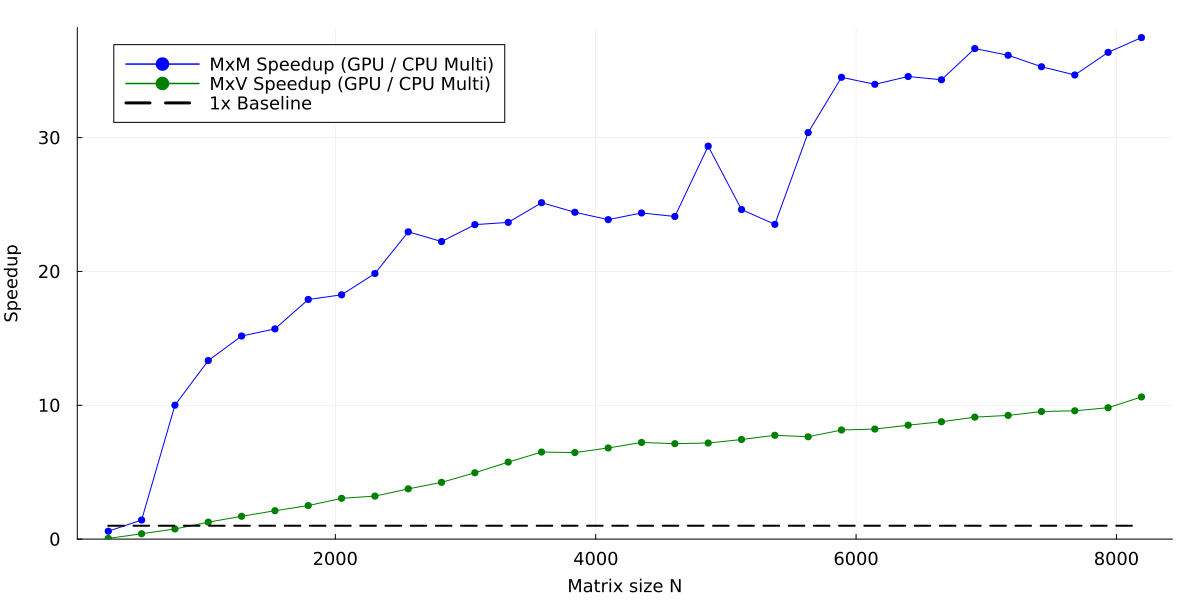
\includegraphics[width=\textwidth]{figures/5_cpu_vs_gpu/Float32_GFLOPS_speedup.png}
\caption{\textbf{FP32 speedup (GPU/CPU): MxM vs.\ MxV.} MxM rapidly enters a high speedup regime as the GPU saturates compute; MxV remains bandwidth-limited and achieves a smaller but noticeable, flatter speedup. We can clearly assume the superiority of GPUs against CPUs for large problem sizes, in both MxM and MxV operations.}
\label{fig:speedup_fp32_ab}
\end{figure}

It is important to clarify that for very large sizes, the speedup widens further mostly because the CPU side falls off (all-core turbo drops, memory pressure rises, thermal throttling and BLAS strategies become less favorable) so CPU GFLOPS decline while the GPU holds steady.

Even we cannot see where the plateau for MxM exactly begins, do not expect the speedup to keep increasing indefinitely with $N$ as this was caused by the GPU's ability to maintain high throughput because of better handling in thermals and libraries, compared to the CPU.

\vspace{2em}

\subsubsection*{(B) FP64: \textnormal{MxM} vs.\ \textnormal{MxV} Speedup}
In FP64, consumer GPUs throttle floating-point throughput, so MxM speedup is much lower than in FP32 even at large $N$: the kernel remains compute-bound, but the architectural FP64 cap limits the attainable advantage over the CPU.

By contrast, MxV is still memory-bound and can exploit the GPU’s much higher memory bandwidth. As a result, its FP64 speedup becomes larger than MxM’s (the gap even flips, having a higher speedup on MxV than MxM).

This is the key takeaway for FP64: compute throttling shrinks MxM’s headroom, while MxV continues to benefit from fast GDDR, yielding a comparatively healthy speedup.

\begin{figure}[H]\centering
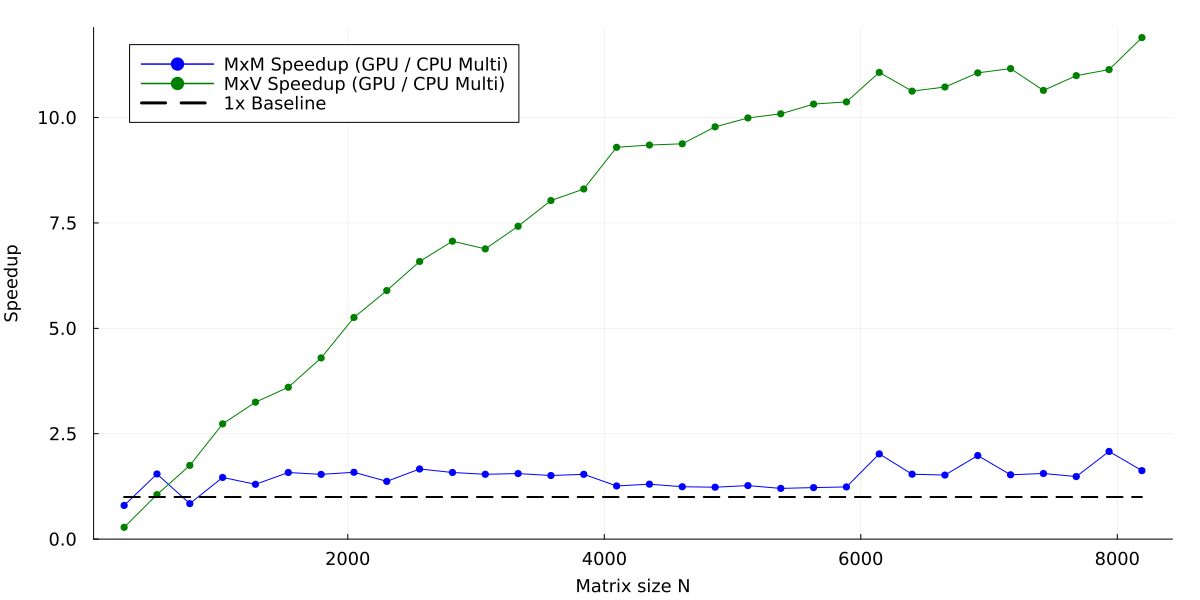
\includegraphics[width=\textwidth]{figures/5_cpu_vs_gpu/Float64_GFLOPS_speedup.png}
\caption{\textbf{FP64 speedup (GPU/CPU): MxM vs.\ MxV.} MxM rapidly enters a high speedup regime as the GPU saturates compute; MxV remains bandwidth-limited and achieves a smaller, flatter speedup.}
\label{fig:speedup_fp64_ab}
\end{figure}
\chapter{Wave Equation 1D with 2nd order finite differences}
\label{ch::chapter6}

\vspace{-1cm}

\section{Introduction to 1D Wave Equation}

We will illustrate this approach using the wave equation as a practical example. The wave equation describes the propagation of waves through a medium and is a fundamental PDE in physics and engineering. It can be expressed in one dimension as:
\begin{equation}
\frac{\partial^2 u}{\partial t^2} = c^2 \frac{\partial^2 u}{\partial x^2}, 
\qquad x\in[0,L],\ t\ge 0,
\label{eq:wave_equation}
\end{equation}
where $u(x,t)$ is the displacement at position $x$ and time $t$, and $c$ is the wave propagation speed.

The initial conditions (IC) are
\begin{align}
u(x,0) &= A\,\exp\!\left(-\frac{(x-x_c)^2}{2\sigma^2}\right), \qquad v(x,0) = 0,
\label{eq:initial_conditions}
\end{align}
and we impose homogeneous Dirichlet boundary conditions (BC) on both fields:
\begin{align}
u(0,t) = u(L,t) = 0, \qquad
v(0,t) = v(L,t) = 0, \qquad t\ge 0.
\label{eq:boundary_conditions}
\end{align}

The wave equation can be reformulated as a first-order system by introducing an auxiliary variable $v(x,t)$, defined as the first time derivative of $u$:
\begin{equation}
v = \frac{\partial u}{\partial t}.
\label{eq:auxiliary_variable}
\end{equation}

Differentiating $u$ once in time, and recognizing the wave equation as a second-order ODE in time, we reformulate it as a coupled system of two first-order PDEs:
\begin{equation}
\begin{aligned}
\frac{\partial u}{\partial t} &= v, \\
\frac{\partial v}{\partial t} &= c^2 \frac{\partial^2 u}{\partial x^2}.
\end{aligned}
\label{eq:coupled_system}
\end{equation}

\clearpage

\subsection{Spatial Discretization: 2nd Order Finite Differences}

We consider a uniform grid $x_i = i \Delta x$ for $i=0,1,\dots,N$, with $\Delta x = L/N$. \\ The second derivative is approximated using a centered stencil as
\begin{equation}
\left.\frac{\partial^2 u}{\partial x^2}\right|_{x=x_i} \approx \frac{u_{i-1} - 2u_i + u_{i+1}}{\Delta x^2}, \quad i=1,\dots,N-1,
\label{eq:second_derivative}
\end{equation}

where $u_i(t) \approx u(x_i,t)$. We will now show how this approximation is derived using Lagrange interpolation. This method involves creating a simple polynomial that fits the function values at nearby points, and then calculating its second derivative to match the given formula.


We approximate $u(x)$ near $x_i$ by the quadratic polynomial $p(x)$ that passes through the points $(x_{i-1}, u_{i-1})$, $(x_i, u_i)$, and $(x_{i+1}, u_{i+1})$, where $x_{i-1} = x_i - \Delta x$, $x_i = i \Delta x$, and $x_{i+1} = x_i + \Delta x$.

The Lagrange polynomial is expressed as
\begin{equation}
\begin{aligned}
p(x) = u_{i-1} \ell_{i-1}(x) + u_i \ell_i(x) + u_{i+1} \ell_{i+1}(x),
\label{eq:lagrange_polynomial}
\end{aligned}
\end{equation}

The Lagrange basis polynomials for points $x_{i-1}$, $x_i$, $x_{i+1}$ are:
\begin{equation}
\begin{aligned}
&\ell_{i-1}(x) = \frac{(x - x_i)(x - x_{i+1})}{(x_{i-1} - x_i)(x_{i-1} - x_{i+1})}, \qquad
\ell_i(x) = \frac{(x - x_{i-1})(x - x_{i+1})}{(x_i - x_{i-1})(x_i - x_{i+1})} \\ \\
&\hspace{7em} \ell_{i+1}(x) = \frac{(x - x_{i-1})(x - x_i)}{(x_{i+1} - x_{i-1})(x_{i+1} - x_i)}.
\end{aligned}
\label{eq:lagrange_basis}
\end{equation}

Shift coordinates so $x_i = 0$, $x_{i-1} = -\Delta x$, $x_{i+1} = \Delta x$. The basis polynomials become
\begin{equation}
\begin{aligned}
\ell_{i-1}(x) = \frac{x (x - \Delta x)}{2 \Delta x^2}, \quad
\ell_i(x) = \frac{\Delta x^2 - x^2}{\Delta x^2}, \quad
\ell_{i+1}(x) = \frac{x (x + \Delta x)}{2 \Delta x^2}.
\end{aligned}
\label{eq:shifted_basis}
\end{equation}

The second derivative is $p''(x) = u_{i-1} \ell_{i-1}''(x) + u_i \ell_i''(x) + u_{i+1} \ell_{i+1}''(x)$. Compute
\begin{equation}
\begin{aligned}
&\ell_{i-1}''(x) = \frac{d^2}{dx^2} \left( \frac{x^2 - x \Delta x}{2 \Delta x^2} \right) = \frac{1}{\Delta x^2}, \qquad
\ell_i''(x) = \frac{d^2}{dx^2} \left( 1 - \frac{x^2}{\Delta x^2} \right) = -\frac{2}{\Delta x^2} \\ \\
&\hspace{7em} \ell_{i+1}''(x) = \frac{d^2}{dx^2} \left( \frac{x^2 + x \Delta x}{2 \Delta x^2} \right) = \frac{1}{\Delta x^2}.
\end{aligned}
\label{eq:second_derivatives}
\end{equation}

At $x = x_i$ (i.e., $x = 0$), 
\begin{equation}
\begin{aligned}
p''(0) = u_{i-1} \cdot \frac{1}{\Delta x^2} + u_i \cdot \left( -\frac{2}{\Delta x^2} \right) + u_{i+1} \cdot \frac{1}{\Delta x^2} = \frac{u_{i-1} - 2u_i + u_{i+1}}{\Delta x^2}.
\end{aligned}
\end{equation}

matching the centered stencil \eqref{eq:second_derivative} we shown earlier.

\clearpage

\subsection{Temporal Discretization}

From the coupled system \eqref{eq:coupled_system}, we can define the state vector $\mathbf{U}$  and the physical vector $\mathbf{F}$ as:

\begin{equation}
\mathbf{U} = \begin{pmatrix} u \\ v \end{pmatrix}, \qquad \mathbf{F} = \begin{pmatrix} v \\ c^2 \frac{\partial^2 u}{\partial x^2} \end{pmatrix}.
\end{equation}

where $u$ and $v$ are the displacement and velocity fields, respectively. The update rule for the state vector can then be expressed as:

\begin{equation}
\mathbf{U}^{n+1} = \mathbf{U}^n + \Delta t \, \mathbf{F}^n,
\end{equation}

\vspace{1em}

This approximation is known as the explicit Euler method. Temporal discretization breaks time into steps (\(\Delta t\)) to approximate the continuous evolution of the system. This process starts by approximating the time derivative of the state vector. Specifically, we use the forward difference

\begin{equation}
\frac{\partial \mathbf{U}}{\partial t} \approx \frac{\mathbf{U}^{n+1} - \mathbf{U}^n}{\Delta t}, \qquad \text{ and setting it equal to } \mathbf{F}^n
\label{eq:time_derivative_approx}
\end{equation}

\vspace{1em}

The explicit Euler method is a first-order accurate time-stepping method. It requires a small \(\Delta t\) for stability and can be adapted to various PDEs with spatial discretization.

This formulation allows us to decouple the physics of the problem from the numerical method used to solve it. The state vector $\mathbf{U}$ contains all relevant information about the system, while the physical vector $\mathbf{F}$ defines the dynamics based on the underlying PDE.

The update rule can be implemented using various numerical methods, such as explicit Euler, implicit Euler, or higher-order Runge-Kutta methods. The choice of method will depend on the specific requirements of the problem, such as stability, accuracy, and computational efficiency.

\clearpage

\section{Code Implementation}
\label{sec:wave_eqn_implementation}

We evolve the solver through four versions in Julia, each building modularity while solving the same problem (explicit finite differences). Code is in \texttt{code/state\_formulation}. This progression introduces the state vector concept basically, from explicit loops to abstract dynamics, preparing for global interpolation in the next chapter.

\subsection{Explicit Implementation}

This is the most basic and transparent implementation of the wave equation solver.

The update equations for $u$ (displacement) and $v$ (velocity) are written explicitly. No modularity or separation of logic (everything is defined inline). There is no use of state vector formulation or external functions.

Initial conditions (Gaussian displacement, zero velocity):
\begin{lstlisting}[language=Julia]
for i in 0:Nx
    x = i * dx
    u[i, 0] = A * exp(-((x - x_c)^2) / (2 * sigma^2))
    v[i, 0] = 0.0
end
\end{lstlisting}

Time integration with Dirichlet boundaries:
\begin{lstlisting}[language=Julia]
for n in 0:Nt-1
    u[0, n] = 0.0; u[Nx, n] = 0.0
    v[0, n] = 0.0; v[Nx, n] = 0.0

    for i in 1:Nx-1
        u[i, n+1] = u[i, n] + dt * v[i, n]
        v[i, n+1] = v[i, n] + dt * c^2 * (u[i+1, n] - 2u[i, n] + u[i-1, n]) / dx^2
    end
end
\end{lstlisting}


\subsection{Modular Implementation}

In this version, we introduce reusable functions to compute the discrete Laplacian, apply boundary conditions, and set the initial state.

Initial conditions:
\begin{lstlisting}[language=Julia]
function apply_initial_conditions(u, v, Nx, dx, A, sigma, x_c)
    for i in 0:Nx
        x = i * dx
        u[i, 0] = A * exp(-((x - x_c)^2) / (2 * sigma^2))
        v[i, 0] = 0.0
    end
    return u, v
end
\end{lstlisting}

\clearpage

Boundaries:
\begin{lstlisting}[language=Julia]
function apply_dirichlet(u, v, n, Nx)
    u[0, n] = 0.0
    u[Nx, n] = 0.0
    v[0, n] = 0.0
    v[Nx, n] = 0.0
    return u, v
end
\end{lstlisting}

Laplacian (second derivative):
\begin{lstlisting}[language=Julia]
function laplacian_1D(u, Nx, dx)
    L = OffsetArray(zeros(Nx + 1), 0:Nx)
    for i in 1:Nx-1
        L[i] = (u[i+1] - 2u[i] + u[i-1]) / dx^2
    end
    return L
end
\end{lstlisting}

First derivative (for energy):
\begin{lstlisting}[language=Julia]
function derivative_1D(u, Nx, dx)
    dudx = OffsetArray(zeros(Nx + 1), 0:Nx)
    for i in 1:Nx-1
        dudx[i] = (u[i+1] - u[i-1]) / (2 * dx)
    end
    return dudx
end
\end{lstlisting}

Time loop:
\begin{lstlisting}[language=Julia]
u, v = apply_initial_conditions(u, v, Nx, dx, A, sigma, x_c)

for n in 0:Nt-1
    u, v = apply_dirichlet(u, v, n, Nx)
    L = laplacian_1D(u[:, n], Nx, dx)

    for i in 1:Nx-1
        u[i, n+1] = u[i, n] + dt * v[i, n]
        v[i, n+1] = v[i, n] + dt * c^2 * L[i]
    end
end
\end{lstlisting}

\emph{\textbf{Note:}} The current 3-point stencil (using $u_{i-1}$, $u_i$, $u_{i+1}$) approximates $\partial^2 u / \partial x^2$ with second-order accuracy. Extend to 5-point ( $u_{i-2}$ to $u_{i+2}$ ) for fourth-order, or more. 

In the next chapter advances to global interpolation, building the precomputed matrices $\mathbf{D}_0$ (interpolation), $\mathbf{D}_1$ (first derivative), $\mathbf{D}_2$ (second derivative), with Lagrange polynomials. But for this chapter, we stick to the 3-point stencil.

\newpage

\subsection{State Vector Implementation}

In this version, we introduce a structural change that brings us closer to general-purpose numerical solvers. Instead of working with two separate arrays—one for the displacement $u$ and one for the velocity $v$, we combine both into a single object: the \textbf{state vector} $U$.

\vspace{0.5em}
\noindent
We define $U$ as a two-dimensional array that stores the full state of the system at each time step. Its rows are split into two regions:
\begin{itemize}
  \item $U[0:Nx, \, :]$ contains the displacement $u$,
  \item $U[Nx+1:2Nx+1, \, :]$ contains the velocity $v$.
\end{itemize}

To keep the familiar notation and make the code readable, we create \texttt{views} over $U$:

\begin{lstlisting}[language=Julia]
N_total = 2 * (Nx + 1)
U = OffsetArray(zeros(N_total, Nt+1), 0:(N_total-1), 0:Nt)
u = OffsetArray(@view(U[0:Nx, :]), (0:Nx, 0:Nt))
v = OffsetArray(@view(U[Nx+1:2Nx+1, :]), (Nx+1:2Nx+1, 0:Nt))
\end{lstlisting}

From this point on, the entire system evolves through $U$, but we can still refer to $u$ and $v$ as if they were separate fields. This improves clarity without sacrificing structure.

The boundary conditions must also reflect this new layout:

\begin{lstlisting}[language=Julia]
function apply_dirichlet(u, v, n, Nx)
    u[0, n] = 0.0
    u[Nx, n] = 0.0
    v[Nx+1, n] = 0.0
    v[2Nx+1, n] = 0.0
    return u, v
end
\end{lstlisting}

Finally, the time-stepping loop is modified to operate on the combined state. Since $v$ is now in the second half of $U$, we must apply an index shift of \texttt{Nx+1} when accessing its values:

\begin{lstlisting}[language=Julia]
for n in 0:Nt-1
    u, v = apply_dirichlet(u, v, n, Nx)
    L = laplacian_1D(u[:, n], Nx, dx)

    for i in 1:Nx-1
        u[i, n+1] = u[i, n] + dt * v[i + (Nx+1), n]
        v[i + (Nx+1), n+1] = v[i + (Nx+1), n] + dt * c^2 * L[i]
    end
end
\end{lstlisting}


This version maintains the same numerical method as before, but rewrites the solver using a more general and scalable data structure. By adopting a state vector, we open the door to more elegant and powerful formulations.

\subsection{Physical Vector Implementation}

In this final version, we fully adopt the dynamical system structure introduced at the beginning of the chapter. We compute an explicit physical vector $F$ at each time step, which contains the time derivatives of all components of the state. The update rule becomes:

\[
\mathbf{U}^{n+1} = \mathbf{U}^n + \Delta t\, \mathbf{F}^n
\]

This approximation, as we already noted, is known as the explicit Euler method.

We use the same state vector layout and each time step, we assemble the physical vector $F$:

\begin{lstlisting}[language=Julia]
for n in 0:Nt-1
    u, v = apply_dirichlet(u, v, n, Nx)
    L = laplacian_1D(u[:, n], Nx, dx)

    @views F[0:Nx] = v[Nx+1:2Nx+1, n]
    @views F[Nx+1:2Nx+1] = c^2 * L

    @views U[:, n+1] = U[:, n] + dt * F
end
\end{lstlisting}

The physical vector $F$ now explicitly represents the right-hand side of the differential equation. Its upper half stores the velocity $v$, while the lower half stores the acceleration $c^2 \cdot \nabla^2 u$.

This structure is clean, extensible, and fully decouples the physics (stored in $F$) from the time-stepping logic. It is a natural starting point for implementing more sophisticated physical models.
% This file is included by main.tex

\chapter{Global Interpolation}
\label{ch::chapter7}

\vspace{-1cm}

\section{Introduction to Global Interpolation}

In numerical methods for partial differential equations (PDEs) such as the wave equation, the accurate approximation of spatial derivatives (e.g., \(\partial u/\partial x\), \(\partial^2 u/\partial x^2\)) on discrete grids is fundamental to solution quality and computational efficiency.

In the previous chapter, we employed explicit 3-node finite difference stencils to approximate derivatives locally. While these stencils are computationally inexpensive and straightforward to implement, they impose several significant limitations like low-order accuracy and rigid grid requirements.

This chapter introduces a fundamentally different approach through \textbf{global interpolation}, implemented via differentiation matrices \(\mathbf{D}_0\), \(\mathbf{D}_1\), and \(\mathbf{D}_2\). Rather than using fixed local stencils, these matrices are constructed using Lagrange basis polynomials that can incorporate information from all grid points simultaneously, hence the term "global."

The key computational advantage of this approach aligns directly with our thesis theme: instead of performing multiple small matrix-vector operations (one per grid point), we can compute all spatial derivatives through a single, large matrix-vector multiplication (in 1D). In 2D this becomes even more pronounced as it is a matrix-matrix multiplication.

The matrices are constructed once at initialization using the Lagrange polynomial algorithm (\texttt{lagrange.jl}), which efficiently computes basis polynomials \(L_j(x)\) and their derivatives \(L_j'(x)\), \(L_j''(x)\) for any desired accuracy order.

We demonstrate the approach using 1D examples, with straightforward extension to multi-dimensional problems. This foundation prepares our solvers for the matrix-matrix formulations that will be crucial for achieving optimal computational performance in the subsequent wave equation implementations.

\clearpage

\section{Lagrange Polynomials}

Lagrange polynomials form the basis for global interpolation. For a set of
nodes $\{x_k\}_{k=0}^{N_x}$, the Lagrange basis polynomial $L_j(x)$ satisfies
$L_j(x_k) = \delta_{jk}$. The interpolated function is:
\begin{equation}
    u(x) \approx \sum_{j=0}^{N_x} u(x_j) L_j(x).
\end{equation}

Where the standard product form for $L_j(x)$ is:
\begin{equation}
    L_j(x) = \prod_{k=0, k \neq j}^{N_x} \frac{x - x_k}{x_j - x_k}.
\end{equation}

We use a iterative formulation that builds $L_j(x)$, $L_j'(x)$, and $L_j''(x)$
incrementally by adding one node at a time to the polynomial from the first
node up to $N_x$.

This starts with a base case with no nodes (q=0): $L = 1$, $L' = 0$, $L'' = 0$.

For each subsequent node $x_k$ (with $k \neq j$), we update:
\begin{equation}
    f(x) = \frac{x - x_k}{x_j - x_k}, \quad f'(x) = \frac{1}{x_j - x_k}, \quad f''(x) = 0.
\end{equation}

Then, applying the product rule to incorporate this factor into the current
partial polynomial $L_m(x)$ (built from the first m nodes), we can build the
polynomial $L(x)$ with $m+1$ nodes:
\begin{equation}
    L(x) = L_m(x) \cdot f(x),
\end{equation}
\begin{equation}
    L'(x) = L_m'(x) \cdot f(x) + L_m(x) \cdot f'(x),
\end{equation}
\begin{equation}
    L''(x) = L_m''(x) \cdot f(x) + 2 L_m'(x) \cdot f'(x) + L_m(x) \cdot f''(x).
\end{equation}

This process is repeated for each node $x_k \neq x_j$, building up to the full
polynomial. When $k = j$, the factor is skipped (effectively $f=1$, $f'=0$,
$f''=0$), ensuring $L_j(x_j) = 1$.

Mathematically, let $L^{(q)}(x)$ be the partial Lagrange polynomial after
including q nodes (excluding $x_j$ itself). The recursion is:
\begin{align}
    L^{(0)}(x)     & = 1, \quad {L^{(0)}}'(x) = 0, \quad {L^{(0)}}''(x) = 0                                          \\
    L^{(q)}(x)     & = L^{(q-1)}(x) \cdot f_q(x)  \label{eq:Lq_iterative}                                                                   \\
    {L^{(q)}}'(x)  & = {L^{(q-1)}}'(x) \cdot f_q(x) + L^{(q-1)}(x) \cdot f_q'(x)  \label{eq:Lq_derivative}                                    \\
    {L^{(q)}}''(x) & = {L^{(q-1)}}''(x) \cdot f_q(x) + 2 {L^{(q-1)}}'(x) \cdot f_q'(x) + L^{(q-1)}(x) \cdot f_q''(x) \label{eq:Lq_second_derivative}
\end{align}

where $f_q(x) = \frac{x - x_{idx_q}}{x_j - x_{idx_q}}$ for the q-th node index
$idx_q \neq j$, \quad $f_q'(x) = \frac{1}{x_j - x_{idx_q}}$, \quad and
$f_q''(x) = 0$. \\

This avoids computing large products directly by accumulating derivatives
step-by-step.

\clearpage

\textbf{Code implementation}

The following Julia code implements an iterative method to compute the Lagrange basis polynomial \( L_j(x) \) and its first and second derivatives (\( L'_j(x) \), \( L''_j(x) \)) at a given point \( x \), using a set of nodes provided in an \texttt{OffsetVector} for zero-based indexing.

\begin{lstlisting}[language=Julia]
using OffsetArrays

function lagrange_derivatives(xnodes::OffsetVector{T,Vector{T}}, j::Int, x::T) where T<:Real
    return iterative_lagrange(xnodes, j, x, length(xnodes))
end

function iterative_lagrange(xnodes::OffsetVector{T,Vector{T}}, j::Int, x::T, q::Int) where T<:Real
    L, dL, ddL = T(1.0), T(0.0), T(0.0)
    keys = collect(axes(xnodes, 1))
    for k in 1:q
        idx = keys[k]
        if idx == j
            continue
        end
        denom = xnodes[j] - xnodes[idx]
        factor = (x - xnodes[idx]) / denom
        dfactor = T(1.0) / denom
        ddfactor = T(0.0)
        
        new_L = L * factor
        new_dL = dL * factor + L * dfactor
        new_ddL = ddL * factor + 2 * dL * dfactor + L * ddfactor
        L, dL, ddL = new_L, new_dL, new_ddL
    end
    return (L, dL, ddL)
end

function evalL(xnodes::OffsetVector{T,Vector{T}}, j::Int, x::T; order::Int=0) where T<:Real
    L, dL, ddL = lagrange_derivatives(xnodes, j, x)
    return order == 0 ? L : order == 1 ? dL : ddL
end
\end{lstlisting}

The function \texttt{iterative\_lagrange} iteratively constructs the Lagrange basis polynomial \( L_j(x) \), along with its first and second derivatives.

The iteration begins with an initial product of 1 (with derivatives set to 0) and processes each node sequentially, applying the product rule to update the polynomial value and its derivatives. By using an iterative approach, the implementation avoids the overhead of recursive function calls, improving performance for large node sets.

The function \texttt{evalL} provides a convenient interface to evaluate \( L_j(x) \) or its derivatives at a specific point \( x \), based on the specified order.

\clearpage

\section{Interpolation Matrix \texorpdfstring{$\mathbf{D}_0$}{D0}}
\label{sec:interp_matrix_D0}


Considering \(\{x_j\}_{j=0}^{M-1}\) as the original (computational) nodes and \(\{x^{\text{interp}}_k\}_{k=0}^{N-1}\) as the new evaluation points
(e.g., a finer grid for visualization). The interpolation matrix
\(\mathbf{D}_0 \in \mathbb{R}^{N\times M}\) is defined so that the interpolated vector
\(\mathbf{u}_{\text{interp}} \in \mathbb{R}^{N}\) (values of \(u\) at the \(x^{\text{interp}}_k\)) is obtained as
\begin{equation}
\mathbf{u}_{\text{interp}} \;=\; \mathbf{D}_0\,\mathbf{u},
\qquad
\mathbf{u} = \big(u(x_0),\dots,u(x_{M-1})\big)^\top.
\end{equation}


\subsection*{Mathematical derivation}
For each \(x^{\text{interp}}_k\) choose a local stencil of \(q\) nodes
\[
S_k \subset \{0,\dots,M-1\}, \qquad |S_k| = q,
\]
e.g., the \(q\) contiguous nodes centered at the node nearest to \(x^{\text{interp}}_k\) (clamped at the boundaries).
On that stencil, define the Lagrange polynomials
\begin{equation}
\ell^{(S_k)}_j(x)
=
\prod_{\substack{m \in S_k\\ m\neq j}}
\frac{x - x_m}{x_j - x_m},
\qquad j \in S_k,
\qquad
\ell^{(S_k)}_j(x) = 0 \ \text{if}\ j \notin S_k.
\label{eq:lagrange_local}
\end{equation}


The \(k\)-th row of \(\mathbf{D}_0\) consists of the interpolation coefficients evaluated at \(x=x^{\text{interp}}_k\):
\begin{equation}
\boxed{\;
\mathbf{D}_0[k,j] \;=\; \ell^{(S_k)}_j(x^{\text{interp}}_k), \qquad j=0,\dots,M-1
\;}
\label{eq:D0_definition}
\end{equation}
Then, for any nodal vector \(\mathbf{u}\),
\begin{equation}
(\mathbf{D}_0 \mathbf{u})_k
\;=\;
\sum_{j=0}^{M-1} \mathbf{D}_0[k,j]\,u(x_j)
\;=\;
\sum_{j\in S_k} \ell^{(S_k)}_j(x^{\text{interp}}_k)\,u(x_j),
\label{eq:row_action}
\end{equation}
which is exactly the \((q-1)\)th degree Lagrange interpolant at \(x^{\text{interp}}_k\) built on stencil \(S_k\).


\subsection*{Global interpolation case}
In the global case we use the same stencil for every row:
\[
S_k \equiv \{0,\dots,M-1\} \qquad (\text{i.e., } q=M,\ \text{independent of }k).
\]
Let \(L_j(x)\) be the global Lagrange basis (note that we used \(\ell^{(S_k)}_j(x)\) when discussing local stencils and now referring to the global case with \(L_j(x)\)) on all \(M\) nodes,
\begin{equation}
L_j(x) \;=\; \prod_{\substack{m=0\\ m\neq j}}^{M-1} \frac{x-x_m}{x_j-x_m},
\qquad j=0,\dots,M-1,
\label{eq:global_lagrange}
\end{equation}
Then every row of \(\mathbf{D}_0\) is just the evaluation of these global basis polynomials at \(x^{\text{interp}}_k\):
\begin{equation}
\boxed{\;
\mathbf{D}_0[k,j] \;=\; L_j(x^{\text{interp}}_k),
\quad k=0,\dots,N-1,\ \ j=0,\dots,M-1
\;}
\label{eq:D0_global_def}
\end{equation}


This \(L_j(x)\) can be computed using the iterative Lagrange formulation we explained in \eqref{eq:Lq_iterative}.

\clearpage

\subsection*{Code implementation}


In the math explanation above we use \(X=\{x_j\}_{j=0}^{M-1}\) (original/computational nodes) and
\(X^{\text{interp}}=\{x^{\text{interp}}_k\}_{k=0}^{N-1}\) (evaluation points).  
In the code, these appear as:
\[
x_j \leftrightarrow \texttt{xnodes[j]}, \qquad
x^{\text{interp}}_k \leftrightarrow \texttt{xinterp[i+1]}.
\]
We choose a stencil \(S_k\) of size \(\texttt{stencil\_size}=q\) with
\texttt{select\_stencil}, and we fill the row \(k\) of \(\mathbf{D}_0\) with the values
\(\ell^{(S_k)}_j(x^{\text{interp}}_k)\) returned by \texttt{iterative\_lagrange} explained above:
\[
\mathbf{D}_0[k,j] \;=\; \ell^{(S_k)}_j(x^{\text{interp}}_k)\qquad\text{(Eq.~\eqref{eq:D0_definition})}
\]



\begin{lstlisting}[language=Julia]
function select_stencil(i::Int, M::Int, q::Int)
    half = div(q, 2)
    imin = clamp(i - half, 0, M - q)
    imax = imin + q - 1
    return imin:imax
end
# xinterp ≠ xnodes
function build_D0_matrix(xnodes::OffsetVector{T,Vector{T}},
                         stencil_size::Int,
                         xinterp::Vector{T}) where T<:Real
    M = length(xnodes)  # Number of nodes.
    N = length(xinterp)  # Number of evaluation points.
    D0 = OffsetArray(zeros(T, N, M), 0:N-1, 0:M-1)  # Initialize matrix.

    for i in 0:N-1
        x = xinterp[i + 1]  # xinterp is 1-based.
        idx_nearest = findmin(abs.(xnodes .- x))[2]
        stencil_range = select_stencil(idx_nearest, M, stencil_size)
        xstencil = OffsetArray(collect(xnodes[stencil_range]), stencil_range)

        for j in stencil_range
            q = length(xstencil)
            lj, _, _ = iterative_lagrange(xstencil, j, x, q)
            D0[i, j] = lj  # Set the basis weight.
        end
    end
    return D0
end
# xinterp = xnodes
function build_D0_matrix(xnodes::OffsetVector{T,Vector{T}},
                         stencil_size::Int) where T<:Real
    build_D0_matrix(xnodes, stencil_size, collect(xnodes))
end
\end{lstlisting}


Each loop over \(k\) builds the \(k\)-th row by evaluating the local Lagrange basis on the
stencil \(S_k\) at \(x^{\text{interp}}_k\), exactly implementing \(\mathbf{D}_0[k,j]=\ell^{(S_k)}_j(x^{\text{interp}}_k)\).
Thus \(\mathbf{D}_0\mathbf{u}\) produces the \((q-1)\)th degree interpolant at all \(x^{\text{interp}}_k\).


With \(\texttt{stencil\_size}=M\), it becomes the global \((M-1)\)th degree interpolant.

\clearpage

\section{First Derivative Matrix \texorpdfstring{$\mathbf{D}_1$}{D1}}
\label{sec:first_derivative_matrix_D1}

Let \(X=\{x_j\}_{j=0}^{M-1}\) be the computational nodes. The first derivative
matrix \(\mathbf{D}_1 \in \mathbb{R}^{M\times M}\) maps nodal samples
\(\mathbf{u}=(u(x_0),\dots,u(x_{M-1}))^\top\) to an approximation of the spatial
derivative \(u_x\) evaluated at the nodes:
\begin{equation}
(\mathbf{D}_1\mathbf{u})_i \;\approx\; \left.\frac{\partial u}{\partial x}\right|_{x=x_i},
\qquad i=0,\dots,M-1.
\end{equation}

\subsection*{Mathematical derivation}
For each target node \(x_i\) choose a local stencil of \(q\) nodes
\[
S_i \subset \{0,\dots,M-1\}, \qquad |S_i|=q,
\]
e.g., the \(q\) contiguous indices centered at \(i\) (clamped at the boundaries).

On that stencil, define the local Lagrange basis \(\{\ell^{(S_i)}_j(x)\}_{j\in S_i}\) by
\begin{equation}
\ell^{(S_i)}_j(x)
=
\prod_{\substack{m \in S_i\\ m\neq j}}
\frac{x - x_m}{x_j - x_m},
\qquad j\in S_i,
\qquad
\ell^{(S_i)}_j(x)=0 \ \text{if } j\notin S_i,
\end{equation}

The derivative at \(x_i\) is approximated by differentiating the local interpolant on \(S_i\)
and evaluating at \(x_i\):


\begin{equation}
\left.\frac{\partial u}{\partial x}\right|_{x=x_i}
\;\approx\;
\sum_{j\in S_i} \ell^{(S_i)\prime}_j(x_i)\,u(x_j).
\end{equation}
Therefore, the entries of \(\mathbf{D}_1\) are
\begin{equation}
\boxed{\;
\mathbf{D}_1[i,j] \;=\; \ell^{(S_i)\prime}_j(x_i),
\qquad i=0,\dots,M-1,\ \ j=0,\dots,M-1
\;}
\label{eq:D1_definition}
\end{equation}
with \(\mathbf{D}_1[i,j]=0\) whenever \(j\notin S_i\). With this definition,
\((\mathbf{D}_1\mathbf{u})_i\) is exactly the derivative of the \((q-1)\)th degree Lagrange
interpolant on \(S_i\) evaluated at \(x_i\).

\subsection*{Global interpolation case}

If \(S_i=\{0,\dots,M-1\}\) for every \(i\) (i.e., \(q=M\)), we obtain the global
first-derivative matrix:

\begin{equation}
\boxed{\;
\mathbf{D}_1[i,j] \;=\; L_j'(x_i)
\;}
\label{eq:D1_global_def}
\end{equation}

where \(L_j(x)\) are the global Lagrange polynomials on all \(M\) nodes. This polynomials derivatives can be obtained using the same iterative Lagrange formulation we explained in \eqref{eq:Lq_derivative}.

In this case of global interpolation, the \(\mathbf{D}_1\) matrix is dense.

\clearpage

\subsection*{Code implementation}
In the math above we use \(X=\{x_j\}_{j=0}^{M-1}\) as the node set and we evaluate the
first derivative at the nodes.
In the code, these appear as:
\[
x_j \leftrightarrow \texttt{xnodes[j]}, \qquad
x_i \ (\text{target node}) \leftrightarrow \texttt{xnodes[i]}.
\]
For each target node \(x_i\) we choose a stencil \(S_i\) of size \(\texttt{stencil\_size}=q\) with
\texttt{select\_stencil(i, M, q)}, build the local node array, and fill row \(i\) of
\(\mathbf{D}_1\) with the first derivatives of the local Lagrange basis at \(x_i\),
returned by \texttt{iterative\_lagrange}.
\[
\mathbf{D}_1[i,j] \;=\; \ell^{(S_i)\prime}_j(x_i)\qquad\text{(Eq.~\eqref{eq:D1_definition})}
\]

\begin{lstlisting}[language=Julia]
function select_stencil(i::Int, M::Int, q::Int)
    half = div(q, 2)
    imin = clamp(i - half, 0, M - q)
    imax = imin + q - 1
    return imin:imax
end

function build_D1_matrix(xnodes::OffsetVector{<:Real}, stencil_size::Int, ::Type{T}=Float64) where T<:Real
    M = length(xnodes)  # Number of nodes.
    D1 = OffsetArray(zeros(T, M, M), 0:M-1, 0:M-1)  # Initialize matrix

    for i in 0:M-1
        stencil_range = select_stencil(i, M, stencil_size)
        xstencil = OffsetArray(convert.(T, collect(xnodes[stencil_range])), stencil_range)

        for j in stencil_range
            q = length(xstencil) 
            _, lp, _ = iterative_lagrange(xstencil, j, T(xnodes[i]), q)
            D1[i, j] = lp  # Set the differentiation weight.
        end
    end

    return D1
end
\end{lstlisting}

Setting \(\texttt{stencil\_size}=M\) yields the global case \(S_i=\{0,\dots,M-1\}\) for all \(i\).

Multiplying \(\mathbf{D}_1\) by the nodal vector \(\mathbf{u}\) returns the
first derivative approximations at all nodes. The same selection logic for
\(\texttt{stencil\_size}\) controls whether the construction is local (sparse/banded) or global (dense).

\clearpage


\section{Second Derivative Matrix \texorpdfstring{$\mathbf{D}_2$}{D2}}
\label{sec:second_derivative_matrix_D2}

Let \(X=\{x_j\}_{j=0}^{M-1}\) be the computational nodes. The second derivative
matrix \(\mathbf{D}_2 \in \mathbb{R}^{M\times M}\) maps nodal samples
\(\mathbf{u}=(u(x_0),\dots,u(x_{M-1}))^\top\) to an approximation of the spatial
second derivative \(u_{xx}\) evaluated at the nodes:
\begin{equation}
(\mathbf{D}_2\mathbf{u})_i \;\approx\; \left.\frac{\partial^2 u}{\partial x^2}\right|_{x=x_i},
\qquad i=0,\dots,M-1.
\end{equation}

\subsection*{Mathematical derivation}
For each target node \(x_i\) choose a local stencil of \(q\) nodes
\[
S_i \subset \{0,\dots,M-1\}, \qquad |S_i|=q,
\]
e.g., the \(q\) contiguous indices centered at \(i\) (clamped at the boundaries).


On that stencil, define the local Lagrange basis \(\{\ell^{(S_i)}_j(x)\}_{j\in S_i}\) by
\begin{equation}
\ell^{(S_i)}_j(x)
=
\prod_{\substack{m \in S_i\\ m\neq j}}
\frac{x - x_m}{x_j - x_m},
\qquad j\in S_i,
\qquad
\ell^{(S_i)}_j(x)=0 \ \text{if } j\notin S_i.
\end{equation}
Differentiate the local interpolant twice and evaluate at \(x_i\):
\begin{equation}
\left.\frac{\partial^2 u}{\partial x^2}\right|_{x=x_i}
\;\approx\;
\sum_{j\in S_i} \ell^{(S_i)\prime\prime}_j(x_i)\,u(x_j).
\end{equation}
Therefore, the entries of \(\mathbf{D}_2\) are
\begin{equation}
\boxed{\;
\mathbf{D}_2[i,j] \;=\; \ell^{(S_i)\prime\prime}_j(x_i),
\qquad i=0,\dots,M-1,\ \ j=0,\dots,M-1
\;}
\label{eq:D2_definition}
\end{equation}
with \(\mathbf{D}_2[i,j]=0\) whenever \(j\notin S_i\). With this definition,
\((\mathbf{D}_2\mathbf{u})_i\) is exactly the second derivative of the degree-\((q-1)\)
Lagrange interpolant on \(S_i\) evaluated at \(x_i\).

\subsection*{Global interpolation case}

If \(S_i=\{0,\dots,M-1\}\) for every \(i\) (i.e., \(q=M\)), we obtain the global
second-derivative matrix:
\begin{equation}
\boxed{\;
\mathbf{D}_2[i,j] \;=\; L_j''(x_i)
\;}
\label{eq:D2_global_def}
\end{equation}
where \(L_j(x)\) are the global Lagrange polynomials on all \(M\) nodes. The values
\(L_j''(x_i)\) can be computed with the iterative Lagrange formulation in
\eqref{eq:Lq_second_derivative}.

In this case of global interpolation, \(\mathbf{D}_2\) is a dense matrix, as it was for \(\mathbf{D}_1\).

\clearpage

\subsection*{Code implementation}
\noindent\textbf{Implementation bridge.}
We evaluate at the nodes themselves (target \(x_i\) and source \(x_j\) are entries of
\texttt{xnodes}). For each row \(i\), we choose \(S_i=\texttt{select\_stencil}(i,M,q)\),
form the local node array, and fill \(\mathbf{D}_2[i,j]\) with the \emph{second derivatives}
returned by \texttt{iterative\_lagrange} at \(x_i\):
\[
\mathbf{D}_2[i,j] \;=\; \ell^{(S_i)\prime\prime}_j(x_i)\qquad\text{(Eq.~\eqref{eq:D2_definition})}
\]

\begin{lstlisting}[language=Julia]
# File: code/interpolants/D2_matrix.jl

using OffsetArrays

include("iterative_lagrange.jl")  # Your module with lagrange_derivatives

function build_D2_matrix(xnodes::OffsetVector{<:Real}, stencil_size::Int, ::Type{T}=Float64) where T<:Real
    M = length(xnodes)  # Number of nodes.
    D2 = OffsetArray(zeros(T, M, M), 0:M-1, 0:M-1)  # Initialize matrix with type T.

    for i in 0:M-1
        # Select stencil centered at i.
        stencil_range = select_stencil(i, M, stencil_size)
        # Create a sub-OffsetArray for the stencil nodes, converting to T.
        xstencil = OffsetArray(convert.(T, collect(xnodes[stencil_range])), stencil_range)

        for j in stencil_range
            q = length(xstencil)  # Actual stencil size.
            _, _, lpp = iterative_lagrange(xstencil, j, T(xnodes[i]), q)
            D2[i, j] = lpp  # Set the differentiation weight.
        end
    end

    return D2
end
\end{lstlisting}

Setting \(\texttt{stencil\_size}=M\) yields the global case \(S_i=\{0,\dots,M-1\}\) for all \(i\).

Multiplying \(\mathbf{D}_2\) by the nodal vector \(\mathbf{u}\) returns the
second derivative approximations at all nodes. The same selection logic for
the local stencils applies here, ensuring that each node's second derivative is computed
using only its neighbors. The choice of \(\texttt{stencil\_size}\) controls again whether the construction is local or global.
% This file is included by main.tex

\chapter{Wave Equation in 1D and 2D with Global Interpolation}
\label{ch::chapter8}

\section{Wave Equation 1D (Matrix–Vector)}
\label{sec:wave_1d_mxv}

\subsection{Mathematical model}

The one-dimensional wave equation can be expressed as:
\begin{equation}
\frac{\partial^2 u}{\partial t^2} = c^2 \frac{\partial^2 u}{\partial x^2}, 
\qquad x\in[0,L],\ t\ge 0,
\label{eq:wave_equation_1d}
\end{equation}

where $u(x,t)$ is the displacement at position $x$ and time $t$, and $c$ is the wave propagation speed. The initial condition and boundary conditions (homogeneous Dirichlet) are specified as:
\begin{align}
u(x,0) &= A\,\exp\!\left(-\frac{(x-x_c)^2}{2\sigma^2}\right), \qquad v(x,0) = 0,
\label{eq:initial_conditions_1d}
\end{align}
\vspace{-0.75em}
\begin{align}
u(0,t) = u(L,t) = 0, \qquad v(0,t) = v(L,t) = 0, \qquad t\ge 0.
\label{eq:boundary_conditions_1d}
\end{align}

where $A$ is the amplitude, $x_c$ is the center position, and $\sigma$ is the width of the initial Gaussian pulse, and $v(x,t) = \frac{\partial u}{\partial t}$ is the velocity field.

The wave equation can be reformulated as a first-order system by introducing the auxiliary variable $v(x,t) = \frac{\partial u}{\partial t}$:
\begin{equation}
\begin{aligned}
\frac{\partial u}{\partial t} &= v, \\
\frac{\partial v}{\partial t} &= c^2 \frac{\partial^2 u}{\partial x^2}.
\end{aligned}
\label{eq:coupled_system_1d}
\end{equation}

\subsubsection*{Spatial discretization (global interpolation)}
We discretize the spatial domain by selecting a set of collocation nodes
\(X=\{x_i\}_{i=0}^{N_x}\subset[0,L]\). The nodes may be uniform or nonuniform (e.g., Chebyshev–Lobatto).

The second derivative at the nodes is represented by the dense matrix \(\mathbf{D}_2^x\in\mathbb{R}^{(N_x+1)\times(N_x+1)}\) whose entries are the second derivatives of the basis functions evaluated at the nodes:
\begin{equation}
\mathbf{D}_2^x[i,j] \;=\; L_j''(x_i),\qquad i,j=0,\dots,N_x
\label{eq:D2x_def_wave}
\end{equation}

i.e., the global case of Eq.~\eqref{eq:D2_global_def}.

Given the nodal vector \(\mathbf{u}(t)=\big(u(x_0,t),\dots,u(x_{N_x},t)\big)^\top\),
the second derivative is approximated at the nodes by the matrix–vector product

\begin{equation}
u_{xx}(\cdot,t)\big|_{X}\;\approx\;\mathbf{D}_2^x\,\mathbf{u}(t).
\label{eq:u_xx_semidiscrete}
\end{equation}

\subsubsection*{Temporal discretization (explicit Euler)}
Writing the first–order system
\(
u_t=v,\quad v_t=c^2\,u_{xx}
\)
and inserting the semidiscrete operator \eqref{eq:u_xx_semidiscrete} gives the
ODE system for the nodal unknowns:
\begin{equation}
\frac{d\mathbf{u}}{dt} \;=\; \mathbf{v},\qquad
\frac{d\mathbf{v}}{dt} \;=\; c^2\,\mathbf{D}_2^x\,\mathbf{u}.
\label{eq:semi_discrete_ode}
\end{equation}

Collect the state at time level \(t^n\) as the stacked vector
\[
\mathbf{U}^{n}
=\begin{pmatrix}\mathbf{u}^{\,n}\\[0.25em]\mathbf{v}^{\,n}\end{pmatrix}
\in \mathbb{R}^{2(N_x+1)},
\qquad
\mathbf{F}^{n}
=\begin{pmatrix}\mathbf{v}^{\,n}\\[0.25em]c^2\,\mathbf{D}_2^x\,\mathbf{u}^{\,n}\end{pmatrix},
\]

so that a forward Euler step with time step \(\Delta t\) reads
\begin{equation}
\mathbf{U}^{\,n+1} \;=\; \mathbf{U}^{\,n} \;+\; \Delta t\,\mathbf{F}^{\,n}.
\label{eq:euler_update}
\end{equation}

This is followed immediately by the strong enforcement of the Dirichlet
constraints at the two boundary nodes for both \(u\) and \(v\).

The time step \(\Delta t\) must satisfy a CFL–like restriction to ensure stability of the explicit advance. This will be enforced by adjusting the time step based on the spatial grid size and wave speed.

\clearpage

\subsection{Code implementation}

The 1D wave solver stores the state in a rank-3 tensor \texttt{U} with shape
\((N_x\!+\!1,\ 2,\ N_t\!+\!1)\):
\begin{itemize}
  \item First dimension: spatial nodes \(x_i\), \(i=0,\dots,N_x\).
  \item Second dimension: fields (index 0 \(\to\) displacement \(u\), index 1 \(\to\) velocity \(v\)).
  \item Third dimension: time levels \(n=0,\dots,N_t\).
\end{itemize}

\noindent The Laplacian in 1D is applied by a single matrix–vector product with the
global second-derivative matrix \(\mathbf{D}_2^x\) from Eq.~\eqref{eq:D2x_def_wave}:
\begin{lstlisting}[language=Julia]
function laplacian_1D(U::OffsetArray{T}, D2x::OffsetArray{T}) where {T}
    return D2x * U[:, 0]
end
\end{lstlisting}
Here, \texttt{U[:, 0]} extracts the displacement vector \(\mathbf{u}^n\in\mathbb{R}^{N_x+1}\)
at the current time step, and \texttt{D2x * U[:, 0]} returns an approximation of
\(\partial^2 u/\partial x^2\) at all nodes (cf. Eq.~\eqref{eq:D2x_def_wave}).

\medskip
\noindent The explicit Euler advance follows the block form in
Eq.~\eqref{eq:euler_update}:
\begin{lstlisting}[language=Julia]
apply_dirichlet!(U, n, Nx)           # enforce homogeneous BCs at t^n
L = laplacian_1D(U[:, :, n], D2x) 

@views begin
    F[:, 0] .= U[:, 1, n]              # RHS for u_t = v
    F[:, 1] .= c^2 .* L                # RHS for v_t = c^2 u_xx
    U[:, :, n+1] .= U[:, :, n] .+ dt .* F
end

apply_dirichlet!(U, n+1, Nx)           # enforce BCs at t^(n+1)
\end{lstlisting}

The working array \texttt{F} has shape \((N_x\!+\!1,2)\) and stores the right-hand
side \(\big[\mathbf{v}^n,\ c^2\mathbf{D}_2^x\mathbf{u}^n\big]\).
Boundary conditions are imposed strongly by overwriting the boundary
entries of \(u\) and \(v\) at each step.

The differentiation matrix \(\mathbf{D}_2^x\) is built once, at startup, via the
global Lagrange construction, choosing a stencil size of \(N_x+1\):
\begin{lstlisting}[language=Julia]
D2x = OffsetArray(build_D2_matrix(xnodes, stencil, T), 0:Nx, 0:Nx)
\end{lstlisting}
Here \texttt{xnodes} holds the collocation nodes (uniform or nonuniform, e.g.,
Chebyshev–Lobatto). With \texttt{stencil\_size = Nx+1} the operator is global
and therefore dense; smaller stencils would yield a banded \(\mathbf{D}_2^x\).
The dominant kernel per step is the BLAS \texttt{gemv} \(\mathbf{D}_2^x\mathbf{u}^n\).

\clearpage

\subsection{Results}

\subsubsection*{Laplacian Operator FP32 Performance}

The isolated 1D Laplacian operator performance demonstrates characteristic memory-bound behavior, consistent with the matrix-vector benchmarks analyzed in Chapter 3.

\vspace{-0.5em}

\begin{figure}[H]\centering
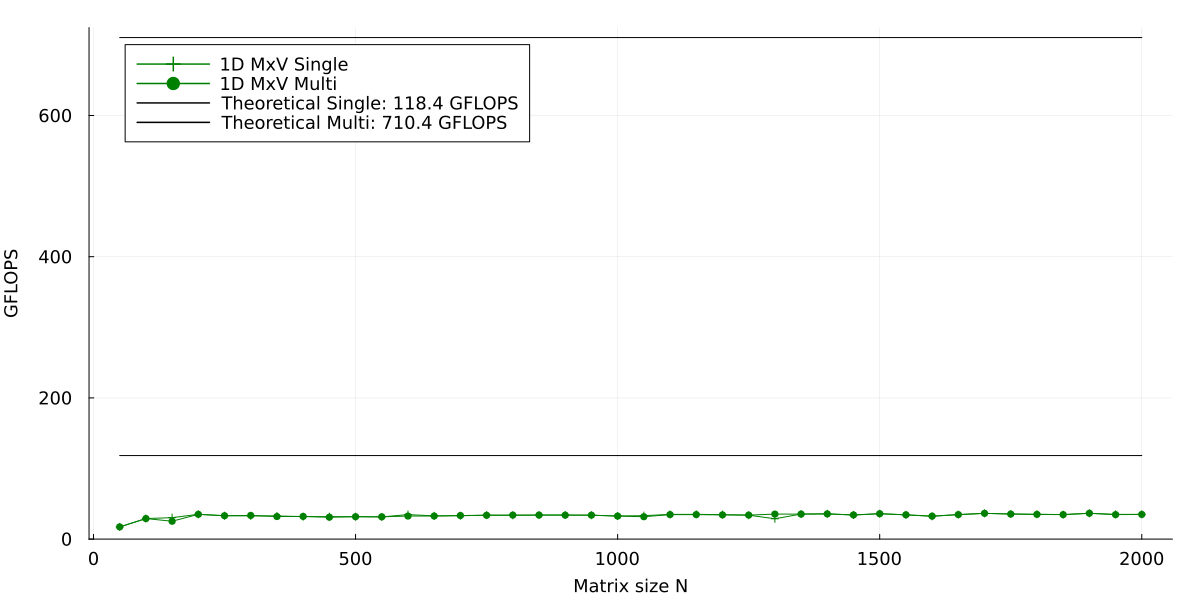
\includegraphics[width=\textwidth]{figures/8_wave_equation_solvers/Float32_GFLOPS_laplacian_1D_MxV.png}
\caption{\textbf{Float32 1D Laplacian (MxV): single vs. multi-threaded performance.} Single-threaded performance shows steady, memory-bound behavior with gradual improvement. Multi-threaded performance closely matches single-threaded initially but exhibits dramatic degradation around mid-range sizes before recovering at larger scales.}
\end{figure}

\textbf{Memory-bound plateau behavior}: Both curves plateau well below compute-bound performance levels, reflecting the low arithmetic intensity inherent to matrix-vector operations. This behavior mirrors the synthetic MxV benchmarks from Chapter 3, where memory bandwidth becomes the fundamental bottleneck regardless of computational resources.

% \textbf{Threading penalty phenomenon}: The sharp multi-threaded performance drop at intermediate sizes demonstrates cache contention effects absent in synthetic benchmarks. Multiple threads competing for the same memory subsystem create bottlenecks that actually reduce performance below single-threaded levels.

\textbf{Consistent single-threaded efficiency}: The stable single-threaded curve across all sizes confirms that memory bandwidth limitation dominates performance, avoiding the complications of inter-thread resource competition.

This 1D implementation validates the theoretical predictions from Chapter 3 regarding matrix-vector limitations, demonstrating that real-world PDE operators exhibit the same fundamental memory-bound characteristics as synthetic benchmarks.

\clearpage

\subsubsection*{1D Wave Equation (MxV) FP64 Performance}

We evaluated the complete 1D wave equation solver across a range of grid sizes using \textbf{Float64 precision} and 1.0 second simulation time. 

Each time step involves matrix-vector multiplication, plus additional operations for temporal integration and boundary condition enforcement. The total floating-point operations per time step can be approximated as \(2 \times N_x^2\) (dominated by the MxV operation):

\begin{equation}
\text{Total Operations} =  \text{Time Steps} \times \text{Operations per Step} \approx N_t \times 2 \times N_x^2
\end{equation}

We used an adaptive time step of $dt = 10^{-4} \times \frac{1}{N_{x}}$ seconds for stability control. This formulation ensures that finer grids use proportionally smaller time steps.

\vspace{1em}


\begin{tabular*}{\linewidth}{@{\extracolsep{\fill}}cccc}
\toprule
\textbf{Grid Size} & \textbf{Time (s)} & \textbf{Total Operations} & \textbf{GFLOPS} \\
\midrule
26 nodes  & 0.10 & 3.52 $\times$ 10$^{8}$  & 3.52 \\
51 nodes  & 0.35 & 2.65 $\times$ 10$^{9}$  & 7.58 \\
76 nodes  & 0.90 & 8.78 $\times$ 10$^{9}$  & 9.76 \\
101 nodes & 1.95 & 2.06 $\times$ 10$^{10}$ & 10.57 \\
126 nodes & 3.66 & 4.00 $\times$ 10$^{10}$ & 10.93 \\
151 nodes & 6.05 & 6.89 $\times$ 10$^{10}$ & 11.38 \\
176 nodes & 8.91 & 1.09 $\times$ 10$^{11}$ & 12.24 \\
201 nodes & 13.47 & 1.62 $\times$ 10$^{11}$ & 12.06 \\
\bottomrule
\end{tabular*}

\vspace{1em}

The performance progression shows consistent scaling behavior across all grid sizes. For small grids (26-76 nodes), we observe steady efficiency improvements as matrix operations begin to dominate computational overhead. The medium grids (101-151 nodes) show continued linear scaling reaching peak efficiency around 11.3 GFLOPS. Finally, large grids (176-201 nodes) exhibit a performance plateau near 12.1 GFLOPS, indicating optimal throughput for this precision.

These results align closely with the Float64 matrix-vector multiplication performance characteristics observed in Chapter 3, confirming that the wave equation solver achieves the expected computational efficiency for dense linear algebra operations. The final performance of approximately 12 GFLOPS demonstrates that the full solver maintains the same computational characteristics as the isolated matrix-vector benchmarks.

\clearpage

\textbf{Physical 1D Wave Evolution (MxV) - Original Nodes Representation}

The solver captures correct wave physics across all stable configurations. Using N=25 nodes with 26-node stencil demonstrates complete wave propagation behavior:

\vspace{0.5em}

\begin{figure}[H]
\centering
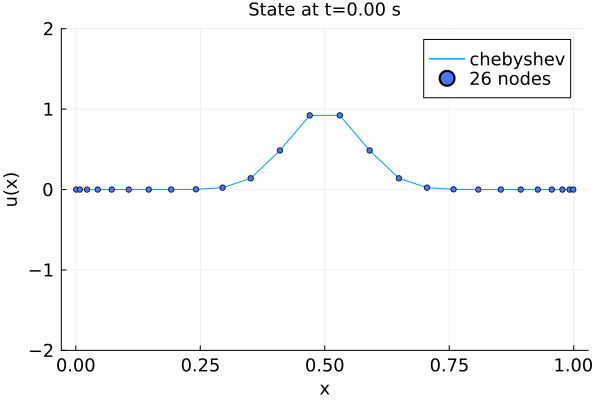
\includegraphics[width=0.48\textwidth]{code/8_wave_equation_solvers/benchmark_versions/output/output1D_25_benchmark/state_t_0.00.png}
\hfill
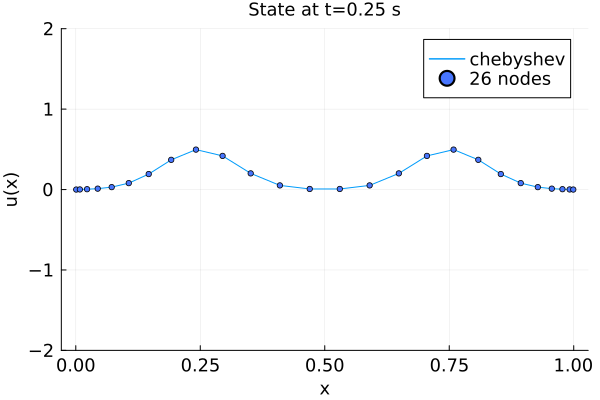
\includegraphics[width=0.48\textwidth]{code/8_wave_equation_solvers/benchmark_versions/output/output1D_25_benchmark/state_t_0.25.png}

\vspace{1em}

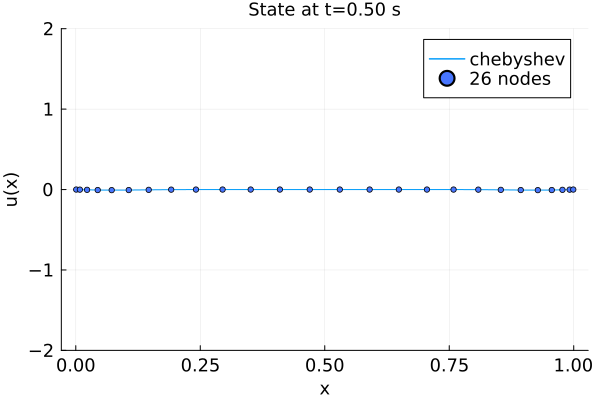
\includegraphics[width=0.48\textwidth]{code/8_wave_equation_solvers/benchmark_versions/output/output1D_25_benchmark/state_t_0.50.png}
\hfill
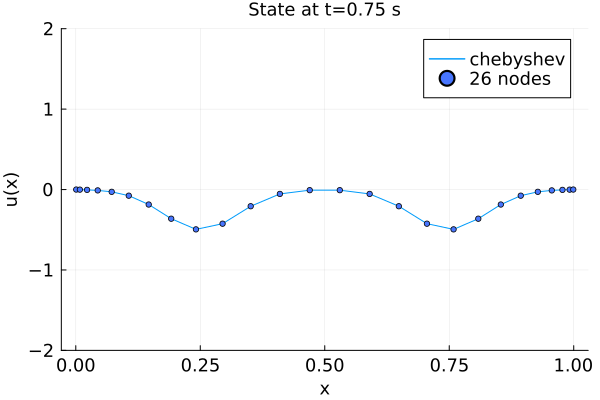
\includegraphics[width=0.48\textwidth]{code/8_wave_equation_solvers/benchmark_versions/output/output1D_25_benchmark/state_t_0.75.png}

\vspace{1em}

\centering
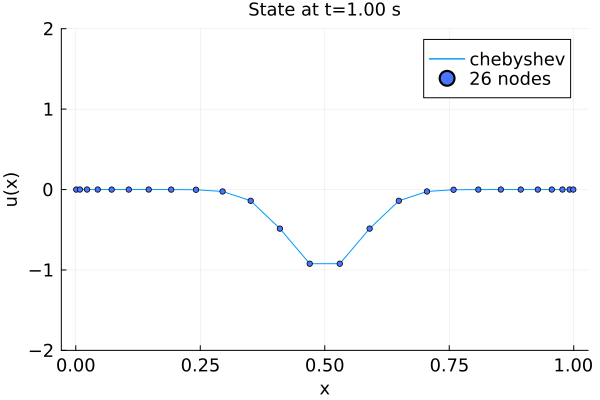
\includegraphics[width=0.48\textwidth]{code/8_wave_equation_solvers/benchmark_versions/output/output1D_25_benchmark/state_t_1.00.png}

\caption{\textbf{1D Wave Equation Evolution.} The temporal sequence shows: (top left) initial Gaussian pulse centered at x = 0.5, (top right) wave splitting into counter-propagating components, (middle left) reflection at Dirichlet boundaries, (middle right) wave interference during convergence, and (bottom) final standing wave configuration. Blue circles indicate the 26 Chebyshev node positions where the discrete solution is computed.}
\end{figure}

\clearpage

\textbf{Physical 1D Wave Evolution (MxV) - Interpolated Representation}

The Chebyshev node distribution enables high-quality Lagrange interpolation to reconstruct the continuous wave field. The solution is interpolated from 26 Chebyshev nodes to 100 equispaced points:

\vspace{0.5em}

\begin{figure}[H]
\centering
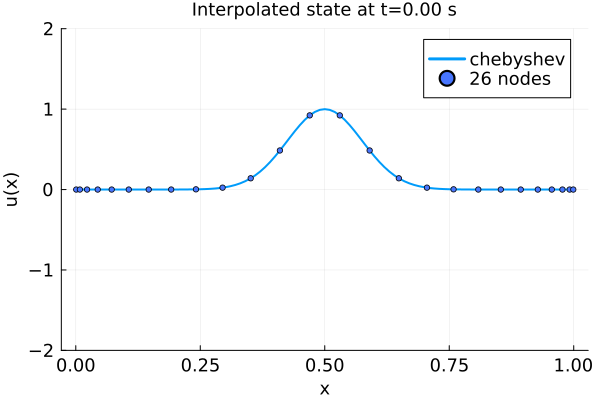
\includegraphics[width=0.48\textwidth]{code/8_wave_equation_solvers/benchmark_versions/output/output1D_25_benchmark/interpolated_state_t_0.00.png}
\hfill
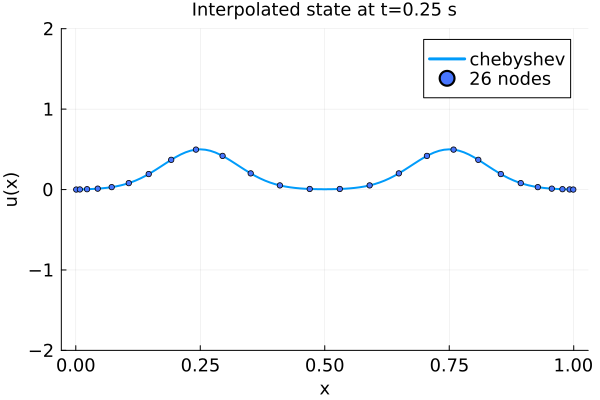
\includegraphics[width=0.48\textwidth]{code/8_wave_equation_solvers/benchmark_versions/output/output1D_25_benchmark/interpolated_state_t_0.25.png}

\vspace{1em}

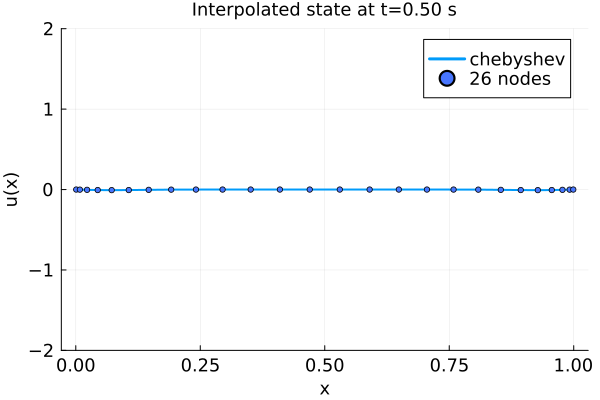
\includegraphics[width=0.48\textwidth]{code/8_wave_equation_solvers/benchmark_versions/output/output1D_25_benchmark/interpolated_state_t_0.50.png}
\hfill
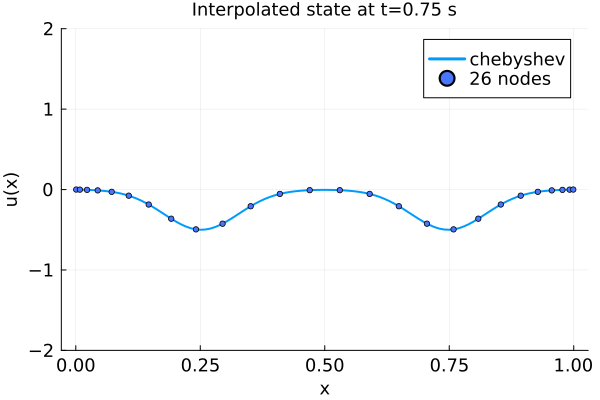
\includegraphics[width=0.48\textwidth]{code/8_wave_equation_solvers/benchmark_versions/output/output1D_25_benchmark/interpolated_state_t_0.75.png}

\vspace{1em}

\centering
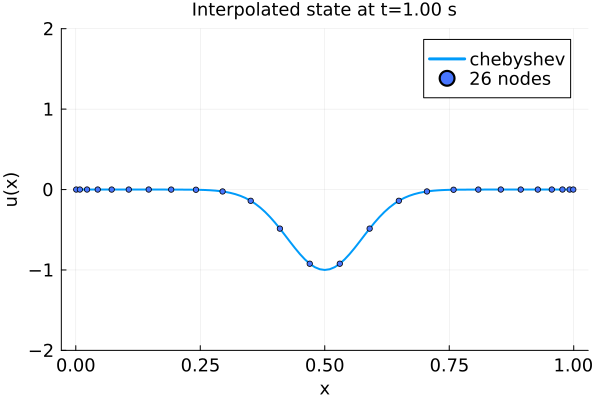
\includegraphics[width=0.48\textwidth]{code/8_wave_equation_solvers/benchmark_versions/output/output1D_25_benchmark/interpolated_state_t_1.00.png}

\caption{\textbf{1D Wave Equation Evolution (Fine Grid).} The continuous curves demonstrate the high accuracy of Lagrange interpolation from the optimal Chebyshev node distribution (blue circles) to a fine equispaced grid of 100 points.}
\end{figure}

\clearpage

\section{Wave Equation 2D (Matrix–Matrix)}
\label{sec:wave_2d_mxm}

\subsection{Mathematical model}

The two-dimensional wave equation can be expressed as:
\begin{equation}
\frac{\partial^2 u}{\partial t^2} = c^2 \left(\frac{\partial^2 u}{\partial x^2} + \frac{\partial^2 u}{\partial y^2}\right), 
\qquad (x,y)\in[0,L_x]\times[0,L_y],\ t\ge 0,
\label{eq:wave_equation_2d}
\end{equation}

where $u(x,y,t)$ is the displacement at position $(x,y)$ and time $t$, and $c$ is the wave propagation speed. The initial condition and boundary conditions (homogeneous Dirichlet) are specified as:
\begin{align}
u(x,y,0) &= A\,\exp\!\left(-\frac{(x-x_c)^2+(y-y_c)^2}{2\sigma^2}\right), \qquad v(x,y,0) = 0,
\label{eq:initial_conditions_2d}
\end{align}
\vspace{-0.75em}
\begin{align}
u(0,y,t) = u(L_x,y,t) = u(x,0,t) = u(x,L_y,t) = 0, \hspace{4.7em}\\
v(0,y,t) = v(L_x,y,t) = v(x,0,t) = v(x,L_y,t) = 0, \qquad t\ge 0.
\label{eq:boundary_conditions_2d}
\end{align}

where $A$ is the amplitude, $(x_c,y_c)$ is the center position, and $\sigma$ is the width of the initial Gaussian pulse, and $v(x,y,t) = \frac{\partial u}{\partial t}$ is the velocity field.

The wave equation can be reformulated as a first-order system by introducing the auxiliary variable $v(x,y,t) = \frac{\partial u}{\partial t}$:
\begin{equation}
\begin{aligned}
\frac{\partial u}{\partial t} &= v, \\
\frac{\partial v}{\partial t} &= c^2 \left(\frac{\partial^2 u}{\partial x^2} + \frac{\partial^2 u}{\partial y^2}\right).
\end{aligned}
\label{eq:coupled_system_2d}
\end{equation}

\subsubsection*{Spatial discretization (global interpolation)}

We discretize the spatial domain using a tensor-product grid by selecting collocation nodes
$X^{(x)}=\{x_i\}_{i=0}^{N_x}\subset[0,L_x]$ and $X^{(y)}=\{y_j\}_{j=0}^{N_y}\subset[0,L_y]$. The nodes may be uniform or nonuniform (e.g., Chebyshev–Lobatto) in each direction.

The 2D Laplacian at grid point $(x_i,y_j)$ splits additively: $\nabla^2 u(x_i,y_j) = u_{xx}(x_i,y_j) + u_{yy}(x_i,y_j)$.

The directional second derivatives are represented by dense matrices $\mathbf{D}_2^x\in\mathbb{R}^{(N_x+1)\times(N_x+1)}$ and $\mathbf{D}_2^y\in\mathbb{R}^{(N_y+1)\times(N_y+1)}$ whose entries are the second derivatives of the basis functions evaluated at the nodes:
\begin{align}
\mathbf{D}_2^x[i,k] &= L_k^{(x)\prime\prime}(x_i),\qquad i,k=0,\dots,N_x \\
\mathbf{D}_2^y[j,\ell] &= L_\ell^{(y)\prime\prime}(y_j),\qquad j,\ell=0,\dots,N_y
\label{eq:D2xy_def_wave}
\end{align}

i.e., the global case of Eq.~\eqref{eq:D2_global_def} applied in each direction.

\clearpage

Given the displacement field as a matrix $\mathbf{U}(t)\in\mathbb{R}^{(N_x+1)\times(N_y+1)}$ with $\mathbf{U}[i,j](t) = u(x_i,y_j,t)$, where rows correspond to different $x_i$ values and columns to different $y_j$ values, the directional derivatives are computed as:
\begin{align}
u_{xx}(\cdot,\cdot,t) &\approx \mathbf{D}_2^x\,\mathbf{U}(t) \qquad \text{(acts on each column, fixed $y_j$)} \\
u_{yy}(\cdot,\cdot,t) &\approx \mathbf{U}(t)\,(\mathbf{D}_2^y)^\top \qquad \text{(acts on each row, fixed $x_i$)}
\end{align}

The transpose in the $y$-derivative appears because $\mathbf{D}_2^y$ is designed to act on column vectors of $y$-direction values, but we need to apply it to each row of $\mathbf{U}$ (corresponding to fixed $x_i$). The matrix multiplication $\mathbf{U}\,(\mathbf{D}_2^y)^\top$ is equivalent to applying $\mathbf{D}_2^y$ to each row vector $\mathbf{U}[i,:]$ and can be understood as:
\[
\big(\mathbf{U}\,(\mathbf{D}_2^y)^\top\big)[i,j] = \sum_{\ell=0}^{N_y} \mathbf{U}[i,\ell] \, (\mathbf{D}_2^y)^\top[\ell,j] = \sum_{\ell=0}^{N_y} \mathbf{D}_2^y[j,\ell] \, u(x_i,y_\ell)
\]
which correctly computes the $y$-derivative at $(x_i,y_j)$ using values along the fixed $x_i$ line.

The 2D Laplacian is then approximated by:
\begin{equation}
\nabla^2 u(\cdot,\cdot,t)\big|_{X^{(x)}\times X^{(y)}}\;\approx\;\mathbf{D}_2^x\,\mathbf{U}(t) + \mathbf{U}(t)\,(\mathbf{D}_2^y)^\top.
\label{eq:laplacian_2d_semidiscrete}
\end{equation}

\subsubsection*{Temporal discretization (explicit Euler)}

Writing the first–order system
$u_t=v$, $v_t=c^2\,(\,u_{xx}+u_{yy})$
and inserting the semidiscrete operator \eqref{eq:laplacian_2d_semidiscrete} gives the
ODE system for the nodal unknowns:
\begin{equation}
\frac{d\mathbf{U}}{dt} \;=\; \mathbf{V},\qquad
\frac{d\mathbf{V}}{dt} \;=\; c^2\,\left(\mathbf{D}_2^x\,\mathbf{U} + \mathbf{U}\,(\mathbf{D}_2^y)^\top\right).
\label{eq:semi_discrete_ode_2d}
\end{equation}

Collect the state at time level $t^n$ as the stacked tensor
\[
\mathbf{U}^{\,n}
=\begin{pmatrix}\mathbf{u}^{\,n}\\\mathbf{v}^{\,n}\end{pmatrix}
\in \mathbb{R}^{(N_x+1)\times(N_y+1)\times 2},
\qquad
\mathbf{F}^{\,n}
=\begin{pmatrix}\mathbf{v}^{\,n}\\c^2\,\left(\mathbf{D}_2^x\,\mathbf{u}^{\,n} + \mathbf{u}^{\,n}\,(\mathbf{D}_2^y)^\top\right)\end{pmatrix},
\]
so that a forward Euler step with time step $\Delta t$ reads
\begin{equation}
\mathbf{U}^{\,n+1} \;=\; \mathbf{U}^{\,n} \;+\; \Delta t\,\mathbf{F}^{\,n}.
\label{eq:euler_update_2d}
\end{equation}

This is followed immediately by the strong enforcement of the Dirichlet
constraints at all four boundary edges for both $u$ and $v$.

In 2D, the choice of $\Delta t$ must satisfy a CFL–like restriction governed by the
smallest grid spacing in both directions, which ensures stability of the explicit advance.

\clearpage

\subsection{Code implementation}

The 2D wave solver stores the state in a rank-4 tensor \texttt{U} with shape
$(N_x\!+\!1,\ N_y\!+\!1,\ 2,\ N_t\!+\!1)$:
\begin{itemize}
  \item First dimension: spatial nodes $x_i$, $i=0,\dots,N_x$.
  \item Second dimension: spatial nodes $y_j$, $j=0,\dots,N_y$.
  \item Third dimension: fields (index 0 $\to$ displacement $u$, index 1 $\to$ velocity $v$).
  \item Fourth dimension: time levels $n=0,\dots,N_t$.
\end{itemize}

\noindent The Laplacian in 2D is applied by two matrix–matrix products with the
global second-derivative matrices $\mathbf{D}_2^x$ and $\mathbf{D}_2^y$ from Eq.~\eqref{eq:D2xy_def_wave}:
\begin{lstlisting}[language=Julia]
function laplacian_2D(U::OffsetArray{T}, D2x::OffsetArray{T}, D2yT::OffsetArray{T}) where {T}
    return D2x * U[:, :, 0] .+ U[:, :, 0] * D2yT
end
\end{lstlisting}
Here, \texttt{U[:, :, 0]} extracts the displacement matrix $\mathbf{u}^n\in\mathbb{R}^{(N_x+1)\times(N_y+1)}$
at the current time step. The operation \texttt{D2x * U[:, :, 0]} applies the x-direction second derivative to each column (fixed $y_j$), while \texttt{U[:, :, 0] * D2yT} applies the y-direction second derivative to each row (fixed $x_i$), returning approximations of $\partial^2 u/\partial x^2$ and $\partial^2 u/\partial y^2$ respectively (cf. Eq.~\eqref{eq:laplacian_2d_semidiscrete}).

\medskip
\noindent The explicit Euler advance follows the block form in
Eq.~\eqref{eq:euler_update_2d}:
\begin{lstlisting}[language=Julia]
apply_dirichlet!(U, n, Nx, Ny)           # enforce homogeneous BCs at t^n
L = laplacian_2D(U[:, :, :, n], D2x, D2yT) 

@views begin
    F[:, :, 0] .= U[:, :, 1, n]           # RHS for u_t = v
    F[:, :, 1] .= c^2 .* L                # RHS for v_t = c^2 (u_xx + u_yy)
    U[:, :, :, n+1] .= U[:, :, :, n] .+ dt .* F
end

apply_dirichlet!(U, n+1, Nx, Ny)         # enforce BCs at t^(n+1)
\end{lstlisting}

The working array \texttt{F} has shape $(N_x\!+\!1,N_y\!+\!1,2)$ and stores $\big[\mathbf{v}^n,\ c^2(\mathbf{D}_2^x\mathbf{u}^n + \mathbf{u}^n(\mathbf{D}_2^y)^\top)\big]$.
Boundary conditions are imposed strongly by overwriting the boundary
entries of $u$ and $v$ at each step on all four edges.

The differentiation matrices $\mathbf{D}_2^x$ and $\mathbf{D}_2^y$ are built once, at startup, via the
global Lagrange construction, choosing stencil sizes of $N_x+1$ and $N_y+1$ respectively:
\begin{lstlisting}[language=Julia]
D2x = OffsetArray(build_D2_matrix(xnodes, Nx+1, T), 0:Nx, 0:Nx)
D2y = OffsetArray(build_D2_matrix(ynodes, Ny+1, T), 0:Ny, 0:Ny)
D2yT = transpose(D2y)
\end{lstlisting}
Here \texttt{xnodes} and \texttt{ynodes} hold the collocation nodes in each direction (uniform or nonuniform, e.g.,
Chebyshev–Lobatto). With \texttt{stencil\_size = Nx+1} and \texttt{Ny+1} the operators are global
and therefore dense; smaller stencils would yield banded matrices.
The dominant kernels per step are the two BLAS \texttt{gemm} operations $\mathbf{D}_2^x\mathbf{u}^n$ and $\mathbf{u}^n(\mathbf{D}_2^y)^\top$.

\clearpage

\subsection{Results}

\subsubsection*{Laplacian Operator FP32 Performance}

The 2D matrix-matrix Laplacian operator demonstrates exceptional computational efficiency, exhibiting behavior consistent with the synthetic benchmarks from Chapter 3.

\vspace{-0.5em}

\begin{figure}[H]\centering
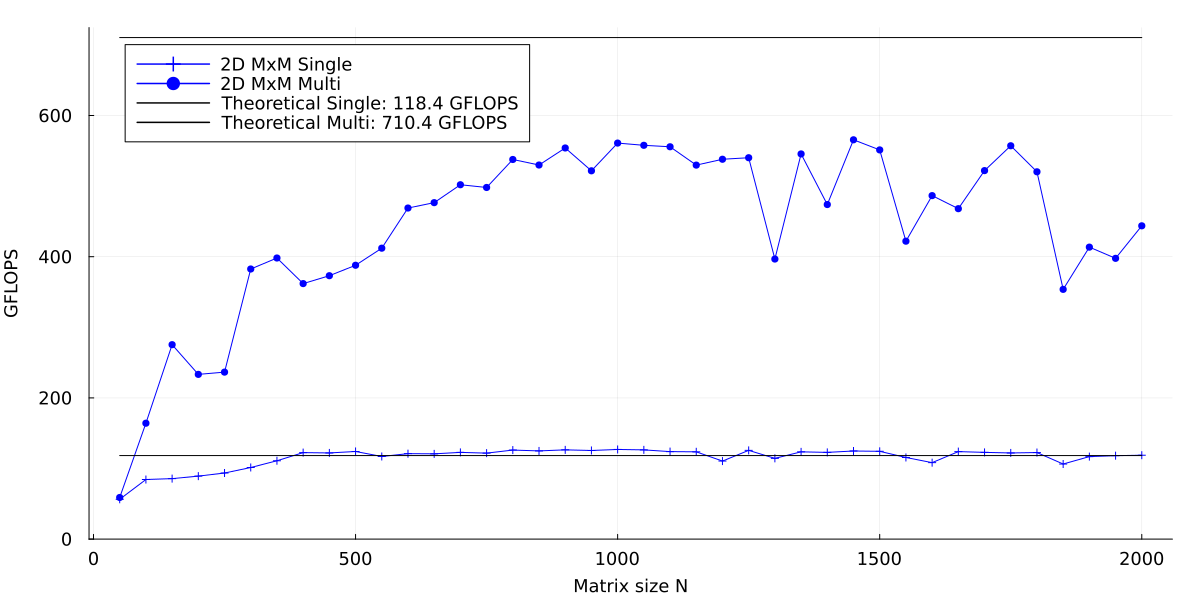
\includegraphics[width=\textwidth]{figures/8_wave_equation_solvers/Float32_GFLOPS_laplacian_2D_MxM.png}
\caption{\textbf{Float32 2D Laplacian (MxM): single vs. multi-threaded performance.} Single-threaded performance steadily improves with matrix size, achieving theoretical performance due to turbo boost effects. Multi-threaded performance shows dramatic scaling with a sharp transition, though remaining below theoretical peaks due to shared resource contention.}
\end{figure}

\textbf{Single-threaded theoretical convergence}: The single-threaded curve reaches and slightly exceeds theoretical performance, mirroring Chapter 3 results. This reflects turbo boost effects where single-core workloads benefit from higher frequencies than base clock calculations assume.

\textbf{Multi-threaded scaling limitations}: Multi-threaded performance exhibits the characteristic sharp transition seen in synthetic benchmarks but remains below theoretical peaks. This gap reflects shared resource contention (L3 cache, memory bandwidth) and lower all-core turbo frequencies, consistent with our earlier analysis.

\textbf{BLAS optimization effectiveness}: The two matrix-matrix products ($\mathbf{D}_2^x\mathbf{u}$ and $\mathbf{u}(\mathbf{D}_2^y)^\top$) achieve compute-bound performance through optimized \texttt{gemm} kernels, demonstrating superior arithmetic intensity compared to matrix-vector alternatives.

The close correspondence with Chapter \ref{ch::chapter3} synthetic results confirms that real-world PDE solvers can achieve predicted computational efficiency when algorithmic structure aligns with modern CPU architectures.

\clearpage

\subsubsection*{2D Wave Equation (MxM) FP64 Performance}

We evaluated the complete 2D wave equation solver across a range of grid sizes using \textbf{Float64 precision} and 1.0 second simulation time.

Each time step involves matrix-matrix multiplication operations, plus additional operations for temporal integration and boundary condition enforcement. The total floating-point operations per time step can be approximated as $2 \times 2 \times N^3$ (dominated by the MxM operations):

\begin{equation}
\text{Total Operations} = \text{Time Steps} \times \text{Operations per Step} \approx N_t \times 2 \times 2 \times N^3
\end{equation}

We used an adaptive time step of $dt = 10^{-4} \times \frac{1}{N_{x}}$ seconds for stability control. This formulation ensures that finer grids use proportionally smaller time steps.

\vspace{0.5em}

\begin{table}[ht]
\centering
\begin{tabular*}{\linewidth}{@{\extracolsep{\fill}}cccc}
\toprule
\textbf{Grid Size} & \textbf{Time (s)} & \textbf{Total Operations} & \textbf{GFLOPS} \\
\midrule
26 nodes  & 6.50   & 1.83 $\times$ 10$^{10}$ & 2.81 \\
51 nodes  & 22.12  & 2.71 $\times$ 10$^{11}$ & 12.23 \\
76 nodes  & 58.44  & 1.33 $\times$ 10$^{12}$ & 22.84 \\
101 nodes & 118.34 & 4.16 $\times$ 10$^{12}$ & 35.17 \\
126 nodes & 207.86 & 1.01 $\times$ 10$^{13}$ & 48.50 \\
151 nodes & 398.64 & 2.08 $\times$ 10$^{13}$ & 52.17 \\
176 nodes & 546.00 & 3.84 $\times$ 10$^{13}$ & 70.29 \\
201 nodes & 919.12 & 6.53 $\times$ 10$^{13}$ & 71.03 \\
\bottomrule
\end{tabular*}
\end{table}


\vspace{1em}

The performance progression demonstrates a scaling behavior across all grid sizes. For small grids (26-76 nodes), we observe rapid efficiency improvements as the cubic scaling of matrix operations begins to dominate computational overhead. The medium grids (101-151 nodes) show continued strong scaling with performance reaching over 50 GFLOPS. Finally, large grids (176-201 nodes) exhibit peak performance near 70 GFLOPS.

This demonstrates the superior computational characteristics of 2D matrix-matrix operations compared to 1D matrix-vector operations. The cubic scaling of operations with grid size ($N^3$) enables higher arithmetic intensity, leading to significantly better GFLOPS performance.

We observe that the performance is still below of what was achieved in the synthetic benchmarks in Chapter 3, likely due to the additional overhead of boundary condition enforcement and temporal integration steps that are not present in isolated matrix-matrix multiplication tests.

\clearpage

\textbf{Physical 2D Wave Evolution (MxM) - Original Nodes Representation}

The 2D solver captures complete wave physics on Chebyshev node grids. Using 25×25 nodes with 26-node stencils demonstrates radial wave propagation and boundary interactions:

\begin{figure}[H]
\centering
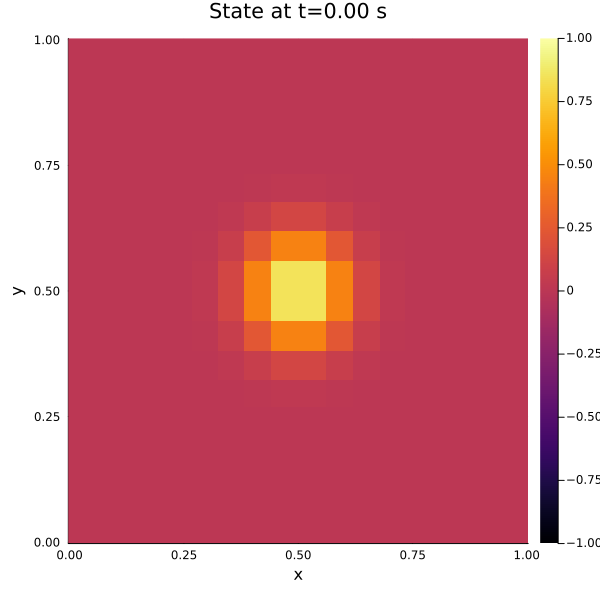
\includegraphics[width=0.48\textwidth]{code/8_wave_equation_solvers/benchmark_versions/output/output2D_25_MxM_benchmark/state_t_0.00.png}
\hfill
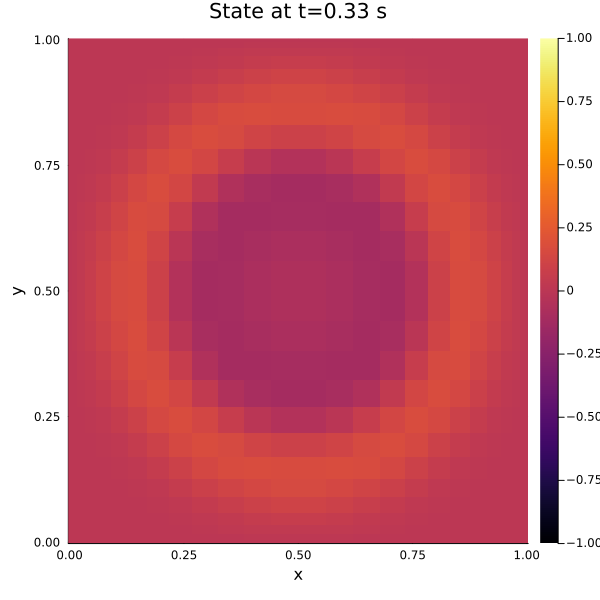
\includegraphics[width=0.48\textwidth]{code/8_wave_equation_solvers/benchmark_versions/output/output2D_25_MxM_benchmark/state_t_0.33.png}

\vspace{1em}

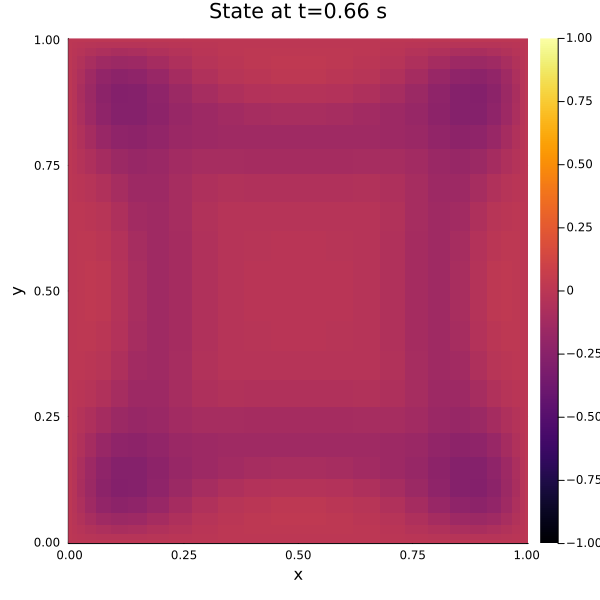
\includegraphics[width=0.48\textwidth]{code/8_wave_equation_solvers/benchmark_versions/output/output2D_25_MxM_benchmark/state_t_0.66.png}
\hfill
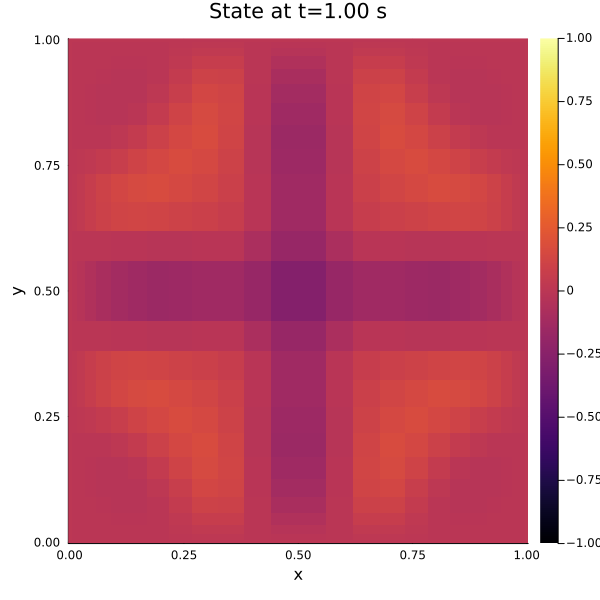
\includegraphics[width=0.48\textwidth]{code/8_wave_equation_solvers/benchmark_versions/output/output2D_25_MxM_benchmark/state_t_1.00.png}

\caption{\textbf{2D Wave Equation Evolution.} The temporal sequence shows: (top left) initial Gaussian pulse centered at domain center, (top right) radial wave expansion at t=0.33s, (bottom left) complex interference patterns at t=0.66s, and (bottom right) final standing wave configuration with multiple nodes at t=1.0s. The discrete solution is computed on a 26×26 Chebyshev node grid.}
\end{figure}

\clearpage

\textbf{Physical 2D Wave Evolution (MxM) - Interpolated Representation}

The 2D Chebyshev node distribution enables high-quality tensor-product Lagrange interpolation to reconstruct the continuous wave field. The solution is interpolated from 26×26 Chebyshev nodes to a 100×100 equispaced grid:

\begin{figure}[H]
\centering
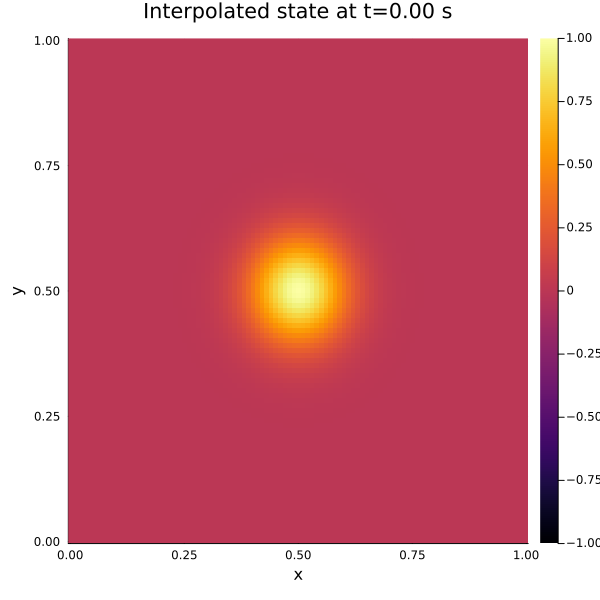
\includegraphics[width=0.48\textwidth]{code/8_wave_equation_solvers/benchmark_versions/output/output2D_25_MxM_benchmark/interpolated_state_t_0.00.png}
\hfill
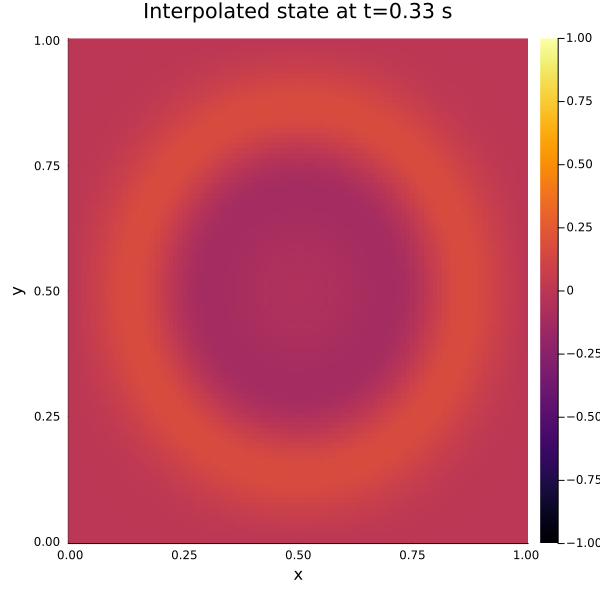
\includegraphics[width=0.48\textwidth]{code/8_wave_equation_solvers/benchmark_versions/output/output2D_25_MxM_benchmark/interpolated_state_t_0.33.png}

\vspace{1em}

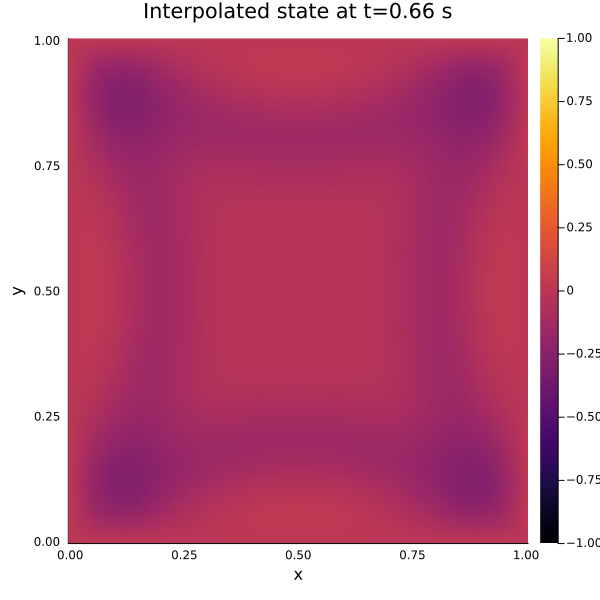
\includegraphics[width=0.48\textwidth]{code/8_wave_equation_solvers/benchmark_versions/output/output2D_25_MxM_benchmark/interpolated_state_t_0.66.png}
\hfill
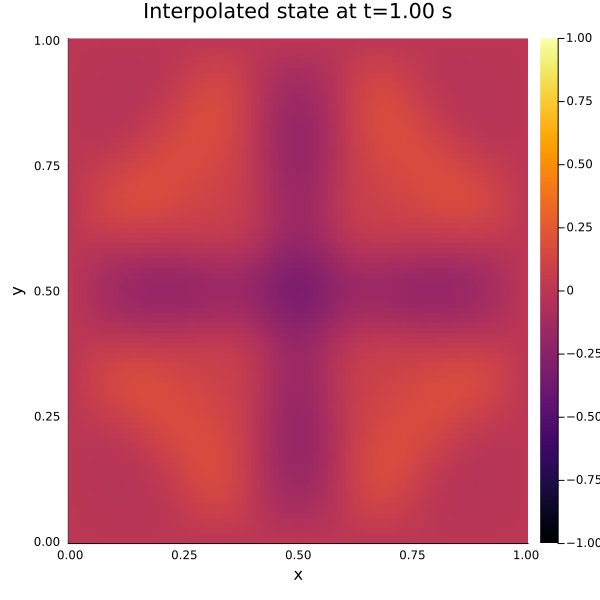
\includegraphics[width=0.48\textwidth]{code/8_wave_equation_solvers/benchmark_versions/output/output2D_25_MxM_benchmark/interpolated_state_t_1.00.png}

\caption{\textbf{2D Wave Equation Evolution. (Fine Grid)} The smooth contours demonstrate excellent interpolation accuracy from the optimal 26×26 Chebyshev node distribution to a fine 100×100 equispaced visualization grid. The tensor-product interpolation preserves wave symmetry and captures fine-scale interference patterns throughout the temporal evolution.}
\end{figure}

\clearpage

\section{Wave Equation 2D (Looped Matrix–Vector)}
\label{sec:wave_2d_mxv}

\subsection{Mathematical model}

The mathematical formulation is identical to Section~\ref{sec:wave_2d_mxm}, solving the 2D wave equation:
\begin{equation}
\frac{\partial^2 u}{\partial t^2} = c^2 \left(\frac{\partial^2 u}{\partial x^2} + \frac{\partial^2 u}{\partial y^2}\right),
\qquad (x,y)\in[0,L_x]\times[0,L_y],\ t\ge 0
\end{equation}

with identical initial and boundary conditions.

The key difference lies in the computational approach for evaluating the Laplacian operator.

\subsubsection*{Alternative Laplacian computation (explicit loops)}

Instead of using the efficient matrix-matrix formulation $\mathbf{D}_2^x\,\mathbf{U} + \mathbf{U}\,(\mathbf{D}_2^y)^\top$, this implementation computes the Laplacian through explicit loops that perform matrix-vector operations for each spatial direction:
\begin{equation}
\nabla^2 u(x_i, y_j) = \sum_{k=0}^{N_x} \mathbf{D}_2^x[i,k] \, u(x_k, y_j) + \sum_{\ell=0}^{N_y} \mathbf{D}_2^y[j,\ell] \, u(x_i, y_\ell)
\end{equation}

This approach mimics applying 1D differentiation operations repeatedly:
\begin{itemize}
    \item For each fixed $y_j$, apply $\mathbf{D}_2^x$ to the vector $\mathbf{u}[:, j]$ (x-direction derivative)
    \item For each fixed $x_i$, apply $\mathbf{D}_2^y$ to the vector $\mathbf{u}[i, :]$ (y-direction derivative)
\end{itemize}

\subsubsection*{Computational complexity}

The looped approach performs $(N_y + 1)$ matrix-vector products for x-direction derivatives, each costing $2(N_x + 1)^2$ FLOPs and $(N_x + 1)$ matrix-vector products for y-direction derivatives, each costing $2(N_y + 1)^2$ FLOPs.

This results in a total of $2(N_x + 1)^2(N_y + 1) + 2(N_x + 1)(N_y + 1)^2 \approx 4M^3$ FLOPs.

While theoretically equivalent to the matrix-matrix approach in FLOP count, the explicit loops result in poorer cache utilization, less efficient use of BLAS routines (\texttt{gemv} vs \texttt{gemm}), and additional loop overhead.

\clearpage

\subsection{Code implementation}

The looped matrix-vector implementation uses the same 4D tensor structure as the matrix-matrix version but computes the Laplacian through explicit nested loops:

\begin{lstlisting}[language=Julia]
function laplacian_2D(U::OffsetArray{T}, n::Int, D2x::OffsetArray{T}, 
                     D2y::OffsetArray{T}, Nx::Int, Ny::Int) where {T}
    L = OffsetArray(zeros(T, Nx+1, Ny+1), 0:Nx, 0:Ny)
    @inbounds @threads for j in 0:Ny
        for i in 0:Nx
            # Compute x-direction second derivative
            d2x = zero(T)
            for ii in 0:Nx
                d2x += D2x[i, ii] * U[ii, j, 0, n]
            end
            # Compute y-direction second derivative
            d2y = zero(T)
            for jj in 0:Ny
                d2y += D2y[j, jj] * U[i, jj, 0, n]
            end
            L[i, j] = d2x + d2y
        end
    end
    return L
end
\end{lstlisting}

Key implementation details:
\begin{itemize}
    \item \texttt{@threads}: Parallelizes the outer loop over $j$ (y-direction)
    \item Inner loops manually compute matrix-vector products using explicit summation
    \item No transpose operation needed for $\mathbf{D}_2^y$ due to explicit indexing structure
\end{itemize}

The time-stepping loop remains identical to the matrix-matrix version:
\begin{lstlisting}[language=Julia]
apply_dirichlet!(U, n, Nx, Ny)           # enforce homogeneous BCs at t^n
L = laplacian_2D(U, n, D2x, D2y, Nx, Ny) 

@views begin
    F[:, :, 0] .= U[:, :, 1, n]           # RHS for u_t = v
    F[:, :, 1] .= c^2 .* L                # RHS for v_t = c^2 (u_xx + u_yy)
    U[:, :, :, n+1] .= U[:, :, :, n] .+ dt .* F
end

apply_dirichlet!(U, n+1, Nx, Ny)         # enforce BCs at t^(n+1)
\end{lstlisting}

The differentiation matrices are built identically to the matrix-matrix version:
\begin{lstlisting}[language=Julia]
D2x = OffsetArray(build_D2_matrix(xnodes, Nx+1, T), 0:Nx, 0:Nx)
D2y = OffsetArray(build_D2_matrix(ynodes, Ny+1, T), 0:Ny, 0:Ny)
\end{lstlisting}

\clearpage

\subsection{Results}

\subsubsection*{Laplacian Operator FP32 Performance}

The 2D looped matrix-vector Laplacian operator consistently demonstrates the poorest performance among all tested approaches, highlighting fundamental algorithmic limitations.

\vspace{-0.5em}

\begin{figure}[H]\centering
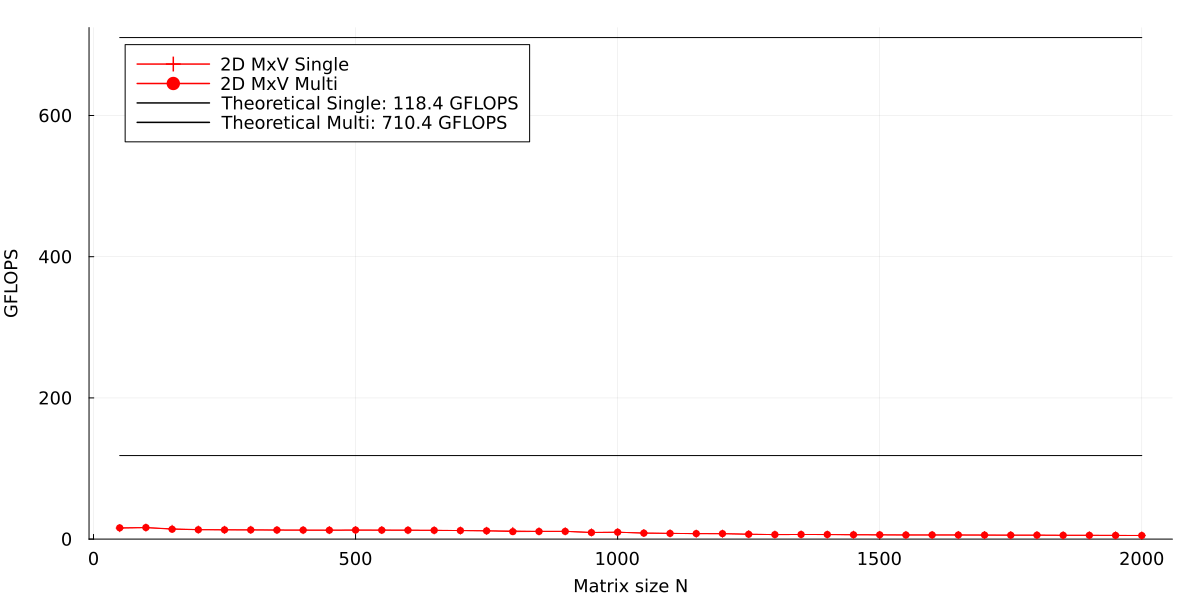
\includegraphics[width=\textwidth]{figures/8_wave_equation_solvers/Float32_GFLOPS_laplacian_2D_MxV.png}
\caption{\textbf{Float32 2D Laplacian (looped MxV): single vs. multi-threaded performance.} Both curves remain consistently low across all matrix sizes, with performance trapped in the 4-16 GFLOPS range. Single-threaded performance shows a declining trend with increasing size, while multi-threaded performance exhibits minimal improvement and similar degradation patterns.}
\end{figure}

\textbf{Consistently poor performance plateau}: Both curves remain trapped well below theoretical and practical performance levels achieved by other approaches, with performance ranging from 4-16 GFLOPS across all tested sizes. Unlike other implementations that show improvement or stability with increasing matrix size, both curves exhibit a general downward trend. Performance drops from peak values around 15-16 GFLOPS at small sizes to 4-6 GFLOPS for larger matrices.

\textbf{Threading ineffectiveness}: The \texttt{@threads} directive provides negligible performance improvements, with multi-threaded results closely tracking single-threaded performance throughout the tested range. This indicates that the explicit loop structure fundamentally limits effective parallelization, preventing the runtime from achieving meaningful speedups despite attempting thread-level parallelism.

This implementation validates the critical importance of algorithmic choice and library optimization, demonstrating that theoretical FLOP equivalence does not guarantee computational efficiency when implementation approaches differ fundamentally in their utilization of modern CPU architectures and optimized libraries.

\clearpage

\subsubsection*{2D Wave Equation (MxV Loop) FP64 Performance}

We evaluated the complete 2D wave equation solver across a range of grid sizes using \textbf{Float64 precision} and 1.0 second simulation time.

Each time step involves matrix-vector multiplication operations, plus additional operations for temporal integration and boundary condition enforcement. The total floating-point operations per time step can be approximated as $2 \times 2 \times N^3$ (dominated by the MxV operations):

\begin{equation}
\text{Total Operations} = \text{Time Steps} \times \text{Operations per Step} \approx N_t \times 2 \times 2 \times N^3
\end{equation}

We used an adaptive time step of $dt = 10^{-4} \times \frac{1}{N_{x}}$ seconds for stability control. This formulation ensures that finer grids use proportionally smaller time steps.

\vspace{1em}

\begin{tabular*}{\linewidth}{@{\extracolsep{\fill}}cccc}
\toprule
\textbf{Grid Size} & \textbf{Time (s)} & \textbf{Total Operations} & \textbf{GFLOPS} \\
\midrule
26 nodes  & 4.84   & 1.83 $\times$ 10$^{10}$ & 3.78 \\
51 nodes  & 30.64  & 2.71 $\times$ 10$^{11}$ & 8.83 \\
76 nodes  & 119.77 & 1.33 $\times$ 10$^{12}$ & 11.14 \\
101 nodes & 350.85 & 4.16 $\times$ 10$^{12}$ & 11.86 \\
126 nodes & 943.62 & 1.01 $\times$ 10$^{13}$ & 10.68 \\
\bottomrule
\end{tabular*}

\vspace{1em}

The performance progression demonstrates a different scaling behavior compared to the MxM implementation across all grid sizes. For small grids (26-51 nodes), we observe steady efficiency improvements as computational overhead is amortized. The medium to large grids (76-126 nodes) show peak performance around 10-11 GFLOPS, with a slight decline for the largest grid size.

This demonstrates the computational characteristics of 2D matrix-vector operations compared to matrix-matrix operations. While the total number of operations remains the same, the MxV implementation shows different performance characteristics due to memory access patterns and computational structure. The peak performance of approximately 11 GFLOPS is significantly lower than the 70 GFLOPS achieved in the MxM benchmark.

The performance plateau and slight decline for larger grids suggests that memory bandwidth limitations become more prominent in MxV operations, where the lower arithmetic intensity compared to MxM operations results in reduced computational throughput.

We observe that the MxV performance is substantially lower than what was achieved in the MxM benchmark, highlighting the importance of algorithmic choice and computational structure in high-performance computing applications, even when the total operation count remains constant.

\clearpage

\textbf{Physical 2D Wave Evolution (MxV) - Original Nodes Representation}

We see exactly the same physical wave evolution as in the matrix-matrix version.

The 2D solver captures complete wave physics on Chebyshev node grids. Using 25×25 nodes with 26-node stencils demonstrates radial wave propagation and boundary interactions:

\begin{figure}[H]
\centering
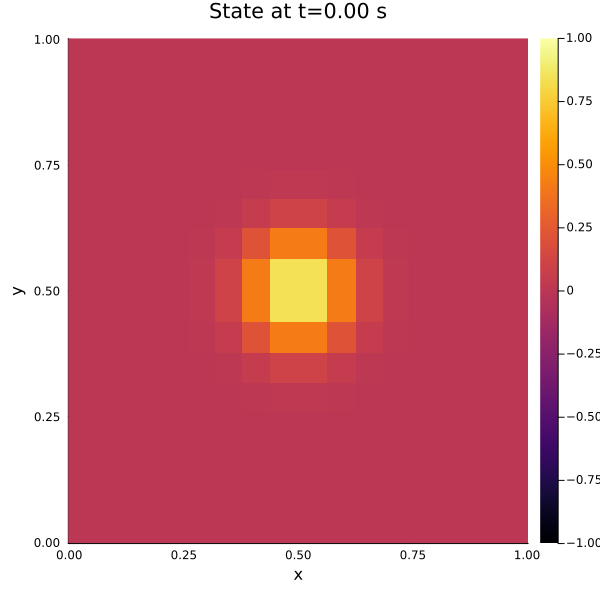
\includegraphics[width=0.48\textwidth]{code/8_wave_equation_solvers/benchmark_versions/output/output2D_25_MxV_benchmark/state_t_0.00.png}
\hfill
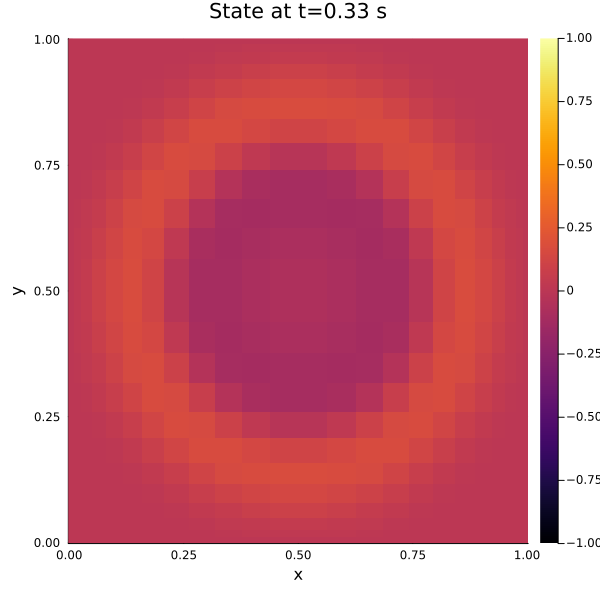
\includegraphics[width=0.48\textwidth]{code/8_wave_equation_solvers/benchmark_versions/output/output2D_25_MxV_benchmark/state_t_0.33.png}

\vspace{1em}

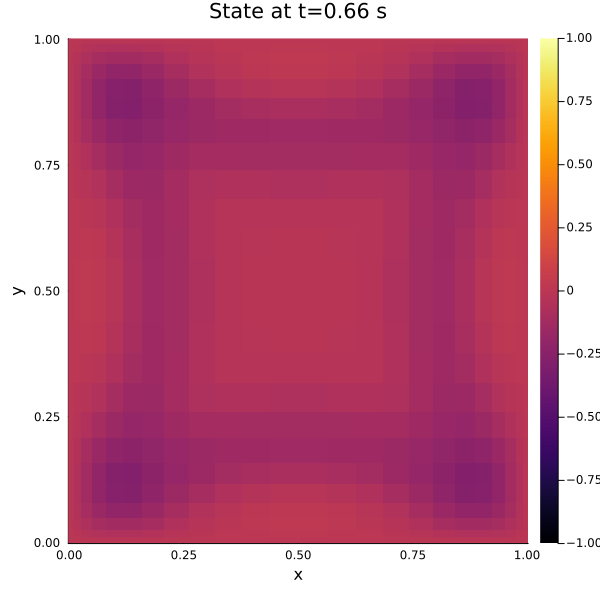
\includegraphics[width=0.48\textwidth]{code/8_wave_equation_solvers/benchmark_versions/output/output2D_25_MxV_benchmark/state_t_0.66.png}
\hfill
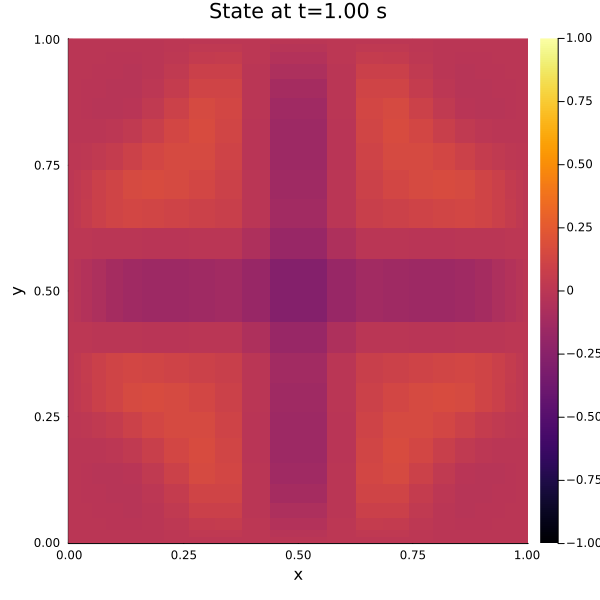
\includegraphics[width=0.48\textwidth]{code/8_wave_equation_solvers/benchmark_versions/output/output2D_25_MxV_benchmark/state_t_1.00.png}

\caption{\textbf{2D Wave Equation Evolution.} The temporal sequence shows: (top left) initial Gaussian pulse centered at domain center, (top right) radial wave expansion at t=0.33s, (bottom left) complex interference patterns at t=0.66s, and (bottom right) final standing wave configuration with multiple nodes at t=1.0s. The discrete solution is computed on a 26×26 Chebyshev node grid.}
\end{figure}

\clearpage

\textbf{Physical 2D Wave Evolution (MxV) - Interpolated Representation}

The 2D Chebyshev node distribution enables high-quality tensor-product Lagrange interpolation to reconstruct the continuous wave field. The solution is interpolated from 26×26 Chebyshev nodes to a 100×100 equispaced grid:

\begin{figure}[H]
\centering
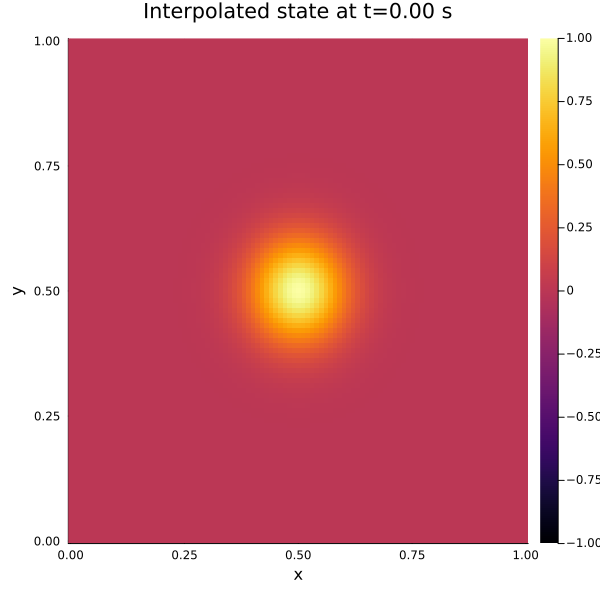
\includegraphics[width=0.48\textwidth]{code/8_wave_equation_solvers/benchmark_versions/output/output2D_25_MxV_benchmark/interpolated_state_t_0.00.png}
\hfill
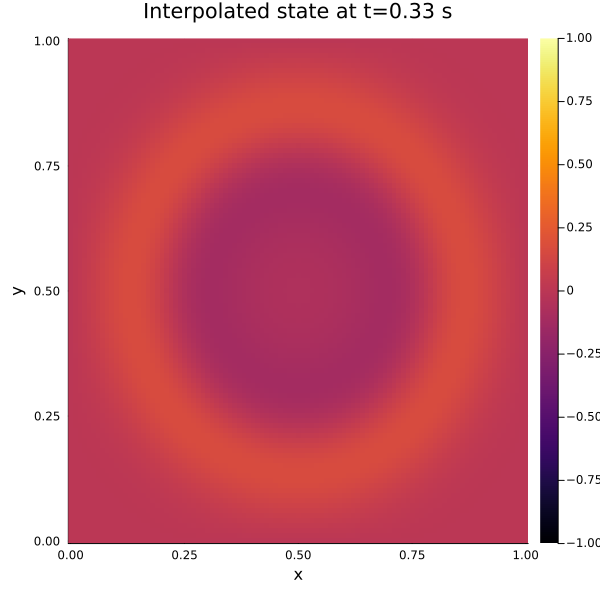
\includegraphics[width=0.48\textwidth]{code/8_wave_equation_solvers/benchmark_versions/output/output2D_25_MxV_benchmark/interpolated_state_t_0.33.png}

\vspace{1em}

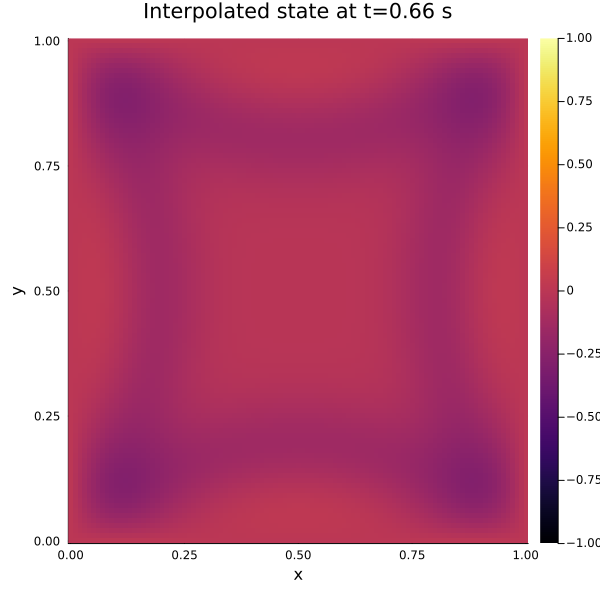
\includegraphics[width=0.48\textwidth]{code/8_wave_equation_solvers/benchmark_versions/output/output2D_25_MxV_benchmark/interpolated_state_t_0.66.png}
\hfill
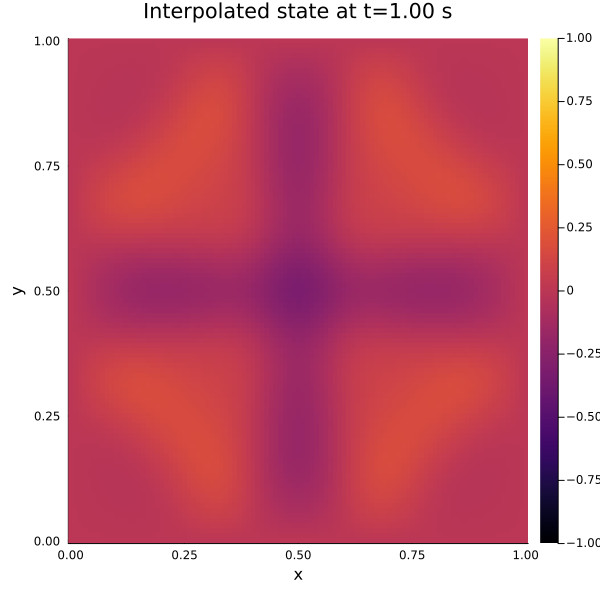
\includegraphics[width=0.48\textwidth]{code/8_wave_equation_solvers/benchmark_versions/output/output2D_25_MxV_benchmark/interpolated_state_t_1.00.png}

\caption{\textbf{2D Wave Equation Evolution (Fine Grid).} The smooth contours demonstrate excellent interpolation accuracy from the optimal 26×26 Chebyshev node distribution to a fine 100×100 equispaced visualization grid. The tensor-product interpolation preserves wave symmetry and captures fine-scale interference patterns throughout the temporal evolution.}
\end{figure}

\clearpage

\section{Wave Equation 2D in NumericalHub (Fortran)}
\label{sec:wave_2d_fortran}

\subsubsection*{2D Wave Equation NumericalHub (Fortran) Performance}

We evaluated the NumericalHub Fortran implementation of the complete 2D wave equation solver across a range of grid sizes using \textbf{Float64 precision} and 1.0 second simulation time. This serves as a benchmark comparison against our custom Julia implementations to assess the relative performance achieved by our developed codes.

The NumericalHub library uses established numerical methods with optimized Fortran implementations. Each time step involves the same fundamental operations as our implementations: spatial differentiation, temporal integration, and boundary condition enforcement. The total floating-point operations per time step follow the same approximation as $2 \times 2 \times N^3$:

\begin{equation}
\text{Total Operations} = \text{Time Steps} \times \text{Operations per Step} \approx N_t \times 2 \times 2 \times N^3
\end{equation}

The same adaptive time step formulation of $dt = 10^{-4} \times \frac{1}{N_{x}}$ seconds is used for stability control, ensuring consistent comparison conditions with our Julia implementations.

\vspace{1em}

\begin{tabular*}{\linewidth}{@{\extracolsep{\fill}}cccc}
\toprule
\textbf{Grid Size} & \textbf{Time (s)} & \textbf{Total Operations} & \textbf{GFLOPS} \\
\midrule
26 nodes & 12.06 & 1.56 $\times$ 10$^{10}$ & 1.29 \\
51 nodes & 228.03 & 2.50 $\times$ 10$^{11}$ & 1.10 \\
76 nodes & 792.80 & 1.27 $\times$ 10$^{12}$ & 1.60 \\
101 nodes & 1812.31 & 4.16 $\times$ 10$^{12}$ & 2.30 \\
\bottomrule
\end{tabular*}

\vspace{1em}

The NumericalHub Fortran implementation demonstrates consistent but modest performance across all grid sizes. Notably, this performance is significantly lower than both our Julia MxM implementation (which achieved up to 70 GFLOPS) and our Julia MxV implementation (which achieved up to 11 GFLOPS).

The comparison reveals several important insights about computational performance. While NumericalHub provides a robust, well-tested library solution, the performance characteristics suggest either more conservative algorithmic choices, additional computational overhead from generalized library functions, or different optimization strategies compared to our specialized implementations.

This performance comparison validates the effectiveness of our custom Julia implementations, demonstrating that targeted optimization and algorithmic design can achieve substantial performance improvements over general-purpose library solutions.

The consistent wave physics results across all implementations confirm that our optimized codes maintain numerical accuracy while delivering superior computational throughput.


\clearpage

\textbf{Physical 2D Wave Evolution (Fortran) Representation}

The 2D wave equation solver demonstrates complete wave physics on a 26×26 Chebyshev node grid. The implementation captures radial wave propagation from a central source and subsequent boundary interactions across the computational domain.

\begin{figure}[H]
\centering
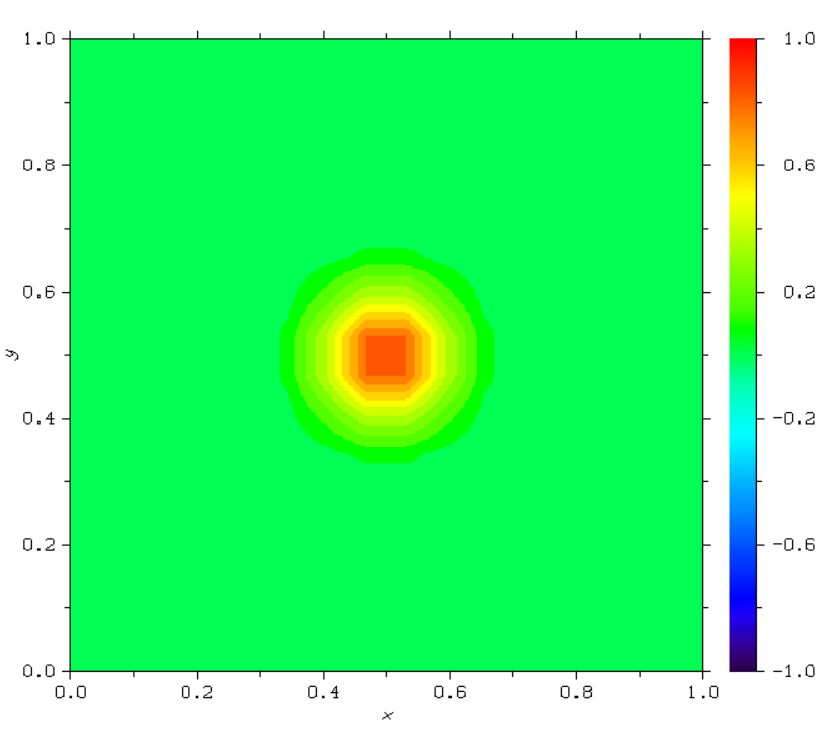
\includegraphics[width=0.48\textwidth]{code/8_wave_equation_solvers/benchmark_versions/output/fortran2D_benchmark/t0.0.png}
\hfill
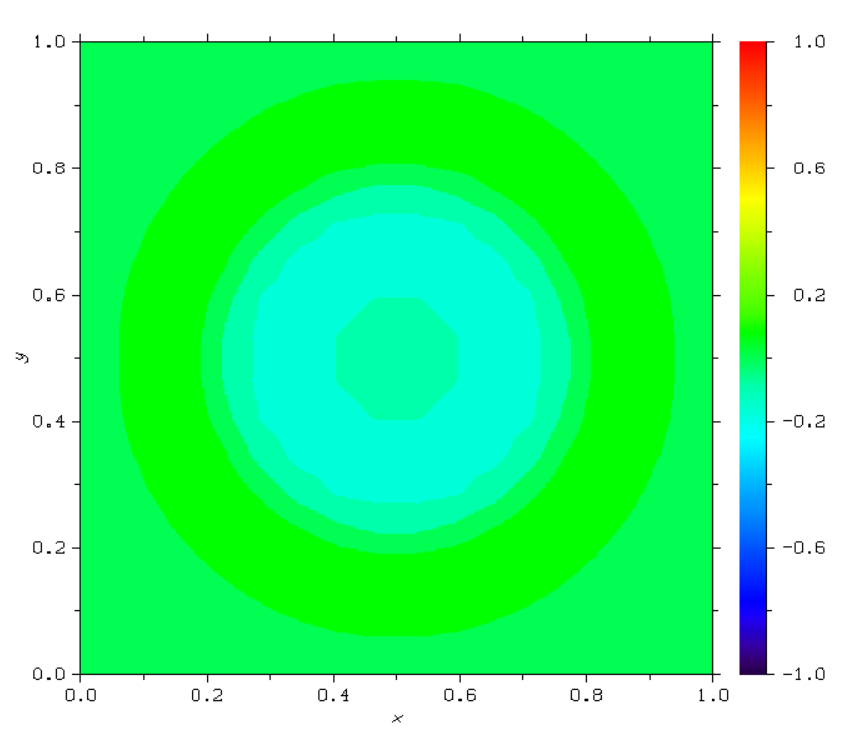
\includegraphics[width=0.48\textwidth]{code/8_wave_equation_solvers/benchmark_versions/output/fortran2D_benchmark/t0.33.png}

\vspace{1em}

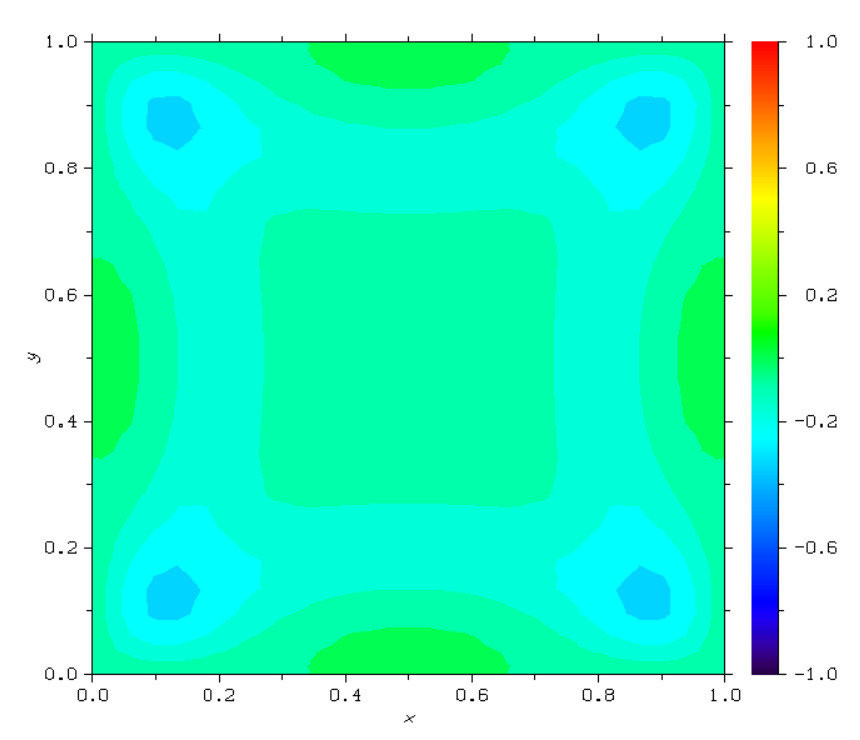
\includegraphics[width=0.48\textwidth]{code/8_wave_equation_solvers/benchmark_versions/output/fortran2D_benchmark/t0.66.png}
\hfill
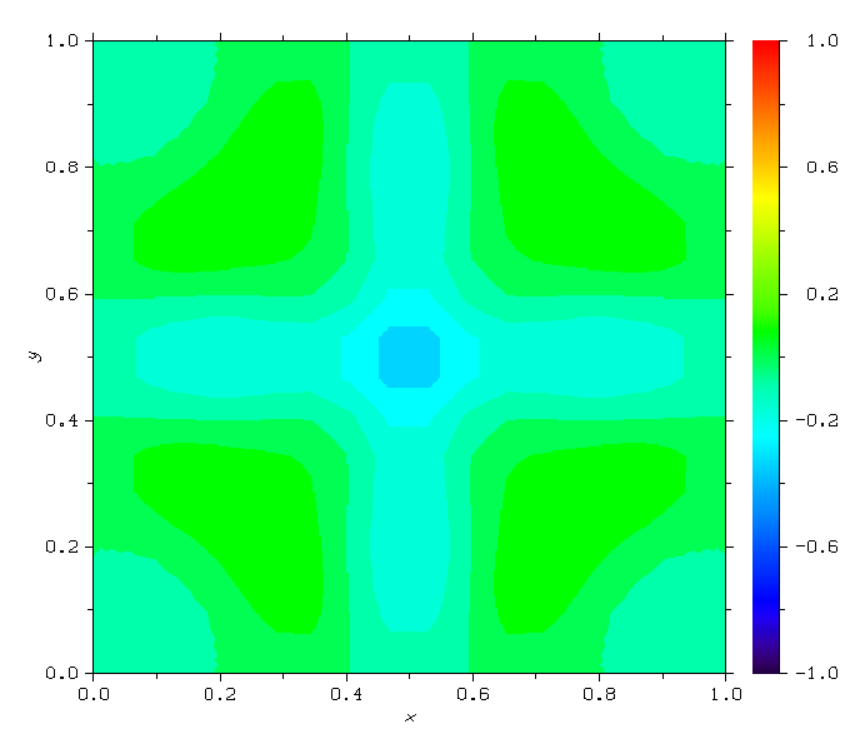
\includegraphics[width=0.48\textwidth]{code/8_wave_equation_solvers/benchmark_versions/output/fortran2D_benchmark/t1.0.png}

\caption{\textbf{2D Wave Equation Evolution.} Numerical solution of the 2D wave equation implemented in NumericalHub and visualized using the plot\_contour function.}
\end{figure}

This visualization represents the same numerical approach implemented in the Julia versions, but executed through the NumericalHub framework with Dislin-based contour plotting for scientific visualization.



% This file is included by main.tex

\chapter{Conclusions}

\label{ch::chapter9}

\vspace{-1cm}

\section{Key Findings and Contributions}

This thesis has conducted a comprehensive investigation into the computational performance characteristics of matrix-vector (MxV) and matrix-matrix (MxM) operations within the context of numerical partial differential equation solvers, with particular emphasis on wave equation implementations across CPU and GPU architectures.

\subsection*{Fundamental Performance Insights}

The central hypothesis of this work (that matrix-matrix formulations achieve superior computational efficiency due to higher arithmetic intensity) has been rigorously validated through both synthetic benchmarks and real-world PDE applications. The theoretical analysis presented in Chapter~\ref{ch::chapter2} established that MxM operations achieve operational intensity scaling as $\mathcal{O}(N)$, while MxV operations saturate at approximately 2 FLOPS per data element. This fundamental difference manifests consistently across all architectural platforms investigated.

On CPU architectures, our benchmarks demonstrate that MxM operations achieve sustained performance approaching theoretical peaks, while MxV operations remain constrained by memory bandwidth limitations, typically plateauing regardless of problem size.

The GPU analysis reveals even more pronounced performance differentials, with MxM operations achieving up to a 30x speedup for large matrices, while MxV performance remains severely bandwidth-bound at substantially lower levels, but still benefits from the higher memory bandwidth of the GPU architecture, allowing up to 10x speedups.

\subsection*{Practical Implications for PDE Solvers}

The transition from 1D to 2D wave equation implementations provides a compelling demonstration of these performance principles in practice. The 1D solver, inherently dominated by matrix-vector operations for spatial differentiation, exhibits characteristic memory-bound behavior with modest GFLOPS rates that plateau as grid resolution increases. In contrast, the 2D matrix-matrix implementation leverages optimized BLAS routines to achieve significant performance improvements, validating the theoretical predictions in a realistic computational physics context.

Particularly noteworthy is the comparison with the reference Fortran implementation from NumericalHub. Despite Fortran's reputation for computational efficiency, our Julia matrix-matrix solver consistently outperforms the reference implementation, demonstrating that algorithmic formulation choices can overcome language-level performance differences.

\subsection*{Architectural Performance Characteristics}

The cross-platform analysis reveals distinct performance profiles across architectures.

CPU implementations benefit significantly from cache-friendly data access patterns in MxM operations, while suffering from cache misses effects in MxV kernels.

GPU architectures amplify these trends: the massive parallelism inherent in GPUs can only be effectively utilized when sufficient arithmetic intensity allows compute units to remain occupied while memory operations proceed in parallel.

The investigation of memory hierarchy effects, including detailed analysis of cache set conflicts and bandwidth limitations, provides valuable insights for performance optimization. The identification of specific grid sizes that trigger cache thrashing (e.g., multiples of 128 for FP32 operations) offers practical guidance for computational grid design.

\subsection*{Global Interpolation as a Unifying Framework}

The development of the global interpolation framework in Chapters~\ref{ch::chapter7} and~\ref{ch::chapter8} represents a significant methodological contribution. By pre-computing differentiation matrices using Lagrange basis polynomials, the framework transforms the traditional node-by-node stencil applications into highly optimized matrix operations. This approach not only improves computational efficiency but also provides a flexible foundation for achieving arbitrary-order accuracy and handling non-uniform grids through Chebyshev node distributions.

The iterative Lagrange polynomial implementation enables efficient computation of high-order differentiation matrices while maintaining numerical stability. The resulting solver architecture clearly separates the physics (encoded in the state tensor $\mathbf{U}$ and physical vector $\mathbf{F}$) from the numerical implementation, facilitating code modularity and extensibility.

\section{Limitations and Scalability Challenges}

The primary constraint lies in the explicit time integration scheme employed throughout this work. The CFL stability condition necessitates time step reductions proportional to spatial grid refinement, resulting in computational cost that scales as $\mathcal{O}(N^4)$ for 2D problems when both spatial and temporal resolutions are considered.

This scaling limitation becomes prohibitive for large-scale simulations (N > 500), where the number of required time steps grows exponentially with grid refinement. Consequently, while MxM operations provide significant per-timestep performance improvements, the overall computational advantage can be offset by stability-imposed time step restrictions in explicit schemes. Additionally, the performance benefits of MxM formulations require sufficiently large matrix dimensions to amortize computational overhead.

\section{Future Work}

\subsection*{Advanced Temporal Integration Schemes}

The most significant limitation of our current approach stems from the use of the explicit Euler method for temporal integration. This simple first-order scheme, while straightforward to implement and understand, imposes severe stability restrictions through the CFL (Courant-Friedrichs-Lewy) condition. When the spatial grid becomes finer (larger $N$), the time step $\Delta t$ must be reduced proportionally to maintain numerical stability.

The path forward requires investigation of temporal integration schemes with significantly larger stability regions. Unlike explicit methods that restrict time steps based on the finest spatial scale, more advanced schemes could allow much larger time steps while maintaining numerical stability.

\subsection*{Full GPU Implementation}

The natural extension of this work involves full GPU implementation of the wave equation solvers using CUDA.jl and cuBLAS. Preliminary analysis suggests that GPU memory bandwidth (448 GB/s on RTX 3070) could provide substantial improvements for memory-bound operations, while the massive parallelism would dramatically accelerate compute-bound MxM kernels.

\cleardoublepage

% --------------------------
% Back matter
% --------------------------
\backmatter

\appendix
\renewcommand{\thechapter}{\Alph{chapter}} % Capítulos como A, B, C...
\renewcommand{\thesection}{\thechapter.\arabic{section}} % Secciones como A.1, A.2...
\chapter{Appendix}
\label{ch::Appendix}

\setcounter{chapter}{1}

\section{Julia programming language initial setup}
\label{sec::JuliaSetup}

This study will be implemented using the Julia programming language.
This section provides an overview of the initial setup required to start programming in Julia.

The Julia programming language is a high-level, high-performance language designed for
numerical and scientific computing. It is known for its speed and ease of use, making
it an ideal choice for developing computational applications. This section provides an
overview of the initial setup required to start programming in Julia.

\subsection{Installation}

The first step in setting up Julia is to download and install the latest version of the language
from the official website (\url{https://julialang.org/downloads/}). The installation process is
straightforward and involves running the installer and following the on-screen instructions.

This will enable you to run Julia code from the command line but to take full advantage, we will use
Visual Studio Code and the Julia extension for Visual Studio Code.

\subsection{Package Management in Julia}

Managing packages efficiently is essential when working on different Julia projects. Julia provides a built-in package manager, \texttt{Pkg}, which allows users to install, update, and manage dependencies. However, to ensure reproducibility and avoid conflicts between projects, it is best to use project-specific environments.

Each Julia project organizes its dependencies using two key files:
\begin{itemize}
    \item \textbf{\texttt{Project.toml}}: Specifies the direct dependencies of the project.
    \item \textbf{\texttt{Manifest.toml}}: Stores the full list of installed packages, including exact versions.
\end{itemize}

Working with project environments ensures that each project has its own set of dependencies,
preventing conflicts between different projects. You will just need the \textbf{\texttt{Project.toml}} file to recreate the environment.


\subsubsection*{Automating Package Management}

To automate package management tasks such as activating environments, resolving
dependencies, and installing required packages, we can use the \texttt{setup.jl} script.

\lstinputlisting[language=Julia, caption=setup.jl]{code/1_annexes/setup.jl}


\section{System Information and Hardware Overview}

It's important to know the system and hardware specifications to know the upper limits of the hardware so that we can compare the results obtained in the benchmarks.

The following code snippets were extracted from the \texttt{system\_info.jl} script, which provides information about the system and hardware specifications.
This script is used to gather information about the system and hardware specifications, such as the operating system, CPU, and GPU details \cite{GPUComputeCapability}.

Function \texttt{cpu\_info(true)} returns the CPU max GFLOPS and function \texttt{gpu\_info(true)} return the GPU max GFLOPS. Using the \texttt{false} argument leds to print the hardware information on the screen.

\begin{lstlisting}[language=Julia, caption=CPU function system\_info.jl]
function cpu_info(return_max_gflops=false)
    N_cores = num_physical_cores()
    N_threads = num_virtual_cores()
    cpuid = cpuinfo()
    string_cpuid = string(cpuid)
    cpu_frequency = 3.7  # GHz (Adjust as needed)
    AVX_value = get_avx_value(string_cpuid)
    M_ops = 4  # 2 FMA, 2 operations each (multiply-add) (AVX2)

    if return_max_gflops
        if AVX_value > 0
            Theoretical_time = 1e9 / (cpu_frequency * 1e9 * AVX_value * M_ops * N_cores)
            max_gflops = 1 / Theoretical_time
            return max_gflops
        else
            return 0
        end
    else
        println("CPU Information")
        println(" ")
        println("CPU Cores: ", N_cores)
        println("CPU Threads: ", N_threads)
        println("CPU Frequency: ", cpu_frequency, " GHz           (GHz adjusted manually)")
        println("AVX support: ", occursin("256 bit", string_cpuid))
        println("AVX-512 support: ", occursin("512 bit", string_cpuid))
        println("AVX Value: ", AVX_value)
        println("M_ops: ", M_ops, " (AVX2: 2 FMA, 2 operations each (multiply-add))")
        if AVX_value > 0
            Theoretical_time = 1e9 / (cpu_frequency * 1e9 * AVX_value * M_ops * N_cores)
            max_gflops = 1 / Theoretical_time
            println("CPU Theoretical max GFLOPS: ", round(max_gflops, digits=2), " GFLOPS (using base frequency)")
        else
            println("AVX not supported. Cannot compute theoretical GFLOPS.")
        end
    end
end
\end{lstlisting}

\begin{lstlisting}[language=Julia, caption=GPU function system\_info.jl]
function gpu_info(return_max_gflops=false)
    device = CUDA.device()
    capability = CUDA.capability(device)
    sm_count = CUDA.attribute(device, CUDA.DEVICE_ATTRIBUTE_MULTIPROCESSOR_COUNT)
    cores_per_sm = cuda_cores_per_sm(capability)
    total_cuda_cores = sm_count * cores_per_sm
    clock_rate = CUDA.attribute(device, CUDA.DEVICE_ATTRIBUTE_CLOCK_RATE) / 1e6

    max_gflops = 2 * clock_rate * total_cuda_cores
    
    memory_clock_khz = CUDA.attribute(device, CUDA.DEVICE_ATTRIBUTE_MEMORY_CLOCK_RATE)
    bus_width_bits = CUDA.attribute(device, CUDA.DEVICE_ATTRIBUTE_GLOBAL_MEMORY_BUS_WIDTH)
    memory_clock_ghz = (memory_clock_khz / 1e6) * 2
    memory_bandwidth = memory_clock_ghz * (bus_width_bits / 8)  # GB/s (8 bits = 1 byte)

    if return_max_gflops
        return max_gflops
    else
        println("GPU Information")
        println(" ")
        println("GPU Name: ", CUDA.name(device))
        println("GPU Compute Capability: ", capability.major, ".", capability.minor, " (", get_GPU_architecture(capability), ")")
        println("GPU Memory: ", round(CUDA.totalmem(device) / 1e9, digits=2), " GB")
        println("GPU Memory: ", round(CUDA.totalmem(device) / 2^30, digits=2), " GiB")
        println("GPU Memory Bandwidth: ", round(memory_bandwidth, digits=2), " GB/s")
        println("GPU Streaming Multiprocessor (SM) Count: ", sm_count)
        println("CUDA Cores per SM: ", cores_per_sm)
        println("Total CUDA Cores: ", total_cuda_cores)
        println("GPU Clock Rate: ", clock_rate, " GHz")
        println("GPU Theoretical max GFLOPS: ", round(max_gflops, digits=2), " GFLOPS")
    end
end
\end{lstlisting}

It's important to modify the \texttt{system\_info.jl} script to include any additional hardware information you want to display and customize parameters as the \texttt{cpu\_frequency} or \texttt{M\_ops}.

\clearpage

\newpage

% called by main.tex
%
\section*{Abbreviations and acronyms}
\label{sec::acronyns}

\vspace{10 mm}
%Institutions
\begin{description}[align=right,labelwidth=2cm] 
\item [UPM] Universidad Politécnica de Madrid
\item [ETSIAE] Escuela Técnica Superior de Ingeniería Aeronáutica y del Espacio
\item [CPU] Central Processing Unit
\item [GPU] Graphics Processing Unit
\item [RAM] Random Access Memory
\item [BLAS] Basic Linear Algebra Subprograms
\item [SMT] Simultaneous Multi-Threading
\item [SIMD] Single Instruction Multiple Data
\item [AVX] Advanced Vector Extensions
\item [SRAM] Static Random Access Memory
\item [DRAM] Dynamic Random Access Memory
\item [FMA] Fused Multiply-Add
\item [BLAS] Basic Linear Algebra Subprograms
\item [CAS] Column Access Strobe
\item [DDR] Double Data Rate
\item [MKL] Math Kernel Library
\item [FLOPS] Floating Point Operations Per Second
\item [MxM] Matrix-Matrix Multiplication
\item [GEMM] General Matrix to Matrix Multiplication
\item [MxV] Matrix-Vector Multiplication
\item [GEMV] General Matrix to Vector Multiplication
\item [VxV] Vector-Vector Multiplication 
\item [FP32] 32-bit Floating Point
\item [FP64] 64-bit Floating Point
\item [HPC] High Performance Computing
\item [PCIe] Peripheral Component Interconnect Express
\item [GT/s] Gigatransfers per Second
\item [BW] Bandwidth
\item [CUDA] Compute Unified Device Architecture
\item [CUs] Compute Units
\item [SMs] Streaming Multiprocessors
\item [GDDR] Graphics Double Data Rate
\item [SIMT] Single Instruction Multiple Threads


\end{description}


\newpage

\nocite{*}
% \bibliographystyle{cas-model2-names}
\bibliographystyle{unsrt} 
\bibliography{references.bib}

% **************************************************
% End of document
% **************************************************
\end{document}
